%!TEX encoding = UTF-8 Unicode

\documentclass[landscape]{book}
\usepackage[a3paper]{geometry}

\usepackage{verbatim}

\usepackage{hyperref}

\usepackage{tikz}

\usetikzlibrary{
  arrows,
  shapes.misc,% wg. rounded rectangle
  shapes.arrows,%
  matrix,%
  scopes,%
  shadows%
}

\tikzset{
  nonterminal/.style={
    % The shape:
    rectangle,
    % The size:
    minimum size=6mm,
    % The border:
    very thick,
    draw=red!50!black!50,         % 50% red and 50% black,
                                  % and that mixed with 50% white
    % The filling:
    top color=white,              % a shading that is white at the top...
    bottom color=red!50!black!20, % and something else at the bottom
    % Font
    font=\itshape\small
  },
  terminal/.style={
    % The shape:
    rounded rectangle,
    minimum size=6mm,
    % The rest
    very thick,draw=black!50,
    top color=white,bottom color=black!20,
    font=\ttfamily\small
  },
  firstPoint/.style={circle,>=stealth',thick,draw=black!50},
  point/.style={coordinate,>=stealth',thick,draw=black!50},
  tip/.style={->,shorten >=0.007pt},
  lastPoint/.style={rectangle,>=stealth',thick,draw=black!50},
  every join/.style={rounded corners}
}

\newcommand\nonTerminalSection[2]{\section{Nonterminal \texttt{#1}}\label{nt:#2}}
\newcommand\ruleSubsection[3]{\subsection{Component \texttt{#1}, in file \texttt{#2}, line #3}}
\newcommand\ruleMatrixColumnSeparation{3mm}
\newcommand\ruleMatrixRowSeparation{3mm}
\newcommand\nonTerminalSymbol[2]{\hyperref[nt:#2]{#1}}
\newcommand\startSymbol[2]{The start symbol is \hyperref[nt:#2]{#1}.}

\newcommand\nonTerminalSummaryStart{This is the alphabetical list of non terminal : }
\newcommand\nonTerminalSummary[2]{\hyperref[nt:#2]{#1}}
\newcommand\nonTerminalSummarySeparator{, }
\newcommand\nonTerminalSummaryEnd{.\\}

\begin{document}

\title{\Huge{Grammar \texttt{galgas4Grammar}}}
\date \today 

\maketitle

\startSymbol{start\_symbol}{30}

\nonTerminalSummaryStart \nonTerminalSummary{actual\_input\_parameter\_list}{19}\nonTerminalSummarySeparator \nonTerminalSummary{actual\_parameter\_list}{13}\nonTerminalSummarySeparator \nonTerminalSummary{actual\_parameter\_list\_within\_parenthesis}{12}\nonTerminalSummarySeparator \nonTerminalSummary{branchOfParseWhithInstruction}{75}\nonTerminalSummarySeparator \nonTerminalSummary{collection\_value\_element}{8}\nonTerminalSummarySeparator \nonTerminalSummary{declaration}{17}\nonTerminalSummarySeparator \nonTerminalSummary{expression}{6}\nonTerminalSummarySeparator \nonTerminalSummary{expression\_and}{10}\nonTerminalSummarySeparator \nonTerminalSummary{expression\_or}{9}\nonTerminalSummarySeparator \nonTerminalSummary{externtype\_constructor}{37}\nonTerminalSummarySeparator \nonTerminalSummary{externtype\_cpp\_classdeclaration}{36}\nonTerminalSummarySeparator \nonTerminalSummary{externtype\_cpp\_predeclaration}{35}\nonTerminalSummarySeparator \nonTerminalSummary{externtype\_getter}{38}\nonTerminalSummarySeparator \nonTerminalSummary{externtype\_method}{40}\nonTerminalSummarySeparator \nonTerminalSummary{externtype\_setter}{39}\nonTerminalSummarySeparator \nonTerminalSummary{factor}{1}\nonTerminalSummarySeparator \nonTerminalSummary{filewrapper\_binary\_files}{33}\nonTerminalSummarySeparator \nonTerminalSummary{filewrapper\_templates}{34}\nonTerminalSummarySeparator \nonTerminalSummary{filewrapper\_text\_files}{32}\nonTerminalSummarySeparator \nonTerminalSummary{for\_instruction\_element}{24}\nonTerminalSummarySeparator \nonTerminalSummary{for\_instruction\_enumerated\_object}{25}\nonTerminalSummarySeparator \nonTerminalSummary{formal\_input\_parameter\_list}{14}\nonTerminalSummarySeparator \nonTerminalSummary{formal\_parameter\_list}{11}\nonTerminalSummarySeparator \nonTerminalSummary{grammar\_instruction\_core}{26}\nonTerminalSummarySeparator \nonTerminalSummary{grammar\_start\_symbol\_label}{76}\nonTerminalSummarySeparator \nonTerminalSummary{gui\_attributes}{68}\nonTerminalSummarySeparator \nonTerminalSummary{gui\_with\_lexique\_declaration}{66}\nonTerminalSummarySeparator \nonTerminalSummary{gui\_with\_option\_declaration}{67}\nonTerminalSummarySeparator \nonTerminalSummary{if\_expression}{15}\nonTerminalSummarySeparator \nonTerminalSummary{if\_instruction\_core}{27}\nonTerminalSummarySeparator \nonTerminalSummary{insert\_or\_replace\_declaration}{43}\nonTerminalSummarySeparator \nonTerminalSummary{issue\_fixit}{23}\nonTerminalSummarySeparator \nonTerminalSummary{label\_formal\_parameter}{77}\nonTerminalSummarySeparator \nonTerminalSummary{lexical\_attribute\_declaration}{59}\nonTerminalSummarySeparator \nonTerminalSummary{lexical\_explicit\_rule}{50}\nonTerminalSummarySeparator \nonTerminalSummary{lexical\_expression}{54}\nonTerminalSummarySeparator \nonTerminalSummary{lexical\_factor}{56}\nonTerminalSummarySeparator \nonTerminalSummary{lexical\_implicit\_rule}{49}\nonTerminalSummarySeparator \nonTerminalSummary{lexical\_indexing\_declaration}{47}\nonTerminalSummarySeparator \nonTerminalSummary{lexical\_instruction}{51}\nonTerminalSummarySeparator \nonTerminalSummary{lexical\_list\_declaration}{57}\nonTerminalSummarySeparator \nonTerminalSummary{lexical\_list\_entry}{58}\nonTerminalSummarySeparator \nonTerminalSummary{lexical\_message\_declaration}{48}\nonTerminalSummarySeparator \nonTerminalSummary{lexical\_output\_effective\_argument}{53}\nonTerminalSummarySeparator \nonTerminalSummary{lexical\_send\_instruction}{64}\nonTerminalSummarySeparator \nonTerminalSummary{lexical\_term}{55}\nonTerminalSummarySeparator \nonTerminalSummary{map\_insert\_setter\_declaration}{44}\nonTerminalSummarySeparator \nonTerminalSummary{method\_declaration}{46}\nonTerminalSummarySeparator \nonTerminalSummary{non\_empty\_output\_expression\_list}{22}\nonTerminalSummarySeparator \nonTerminalSummary{nonterminal\_declaration}{69}\nonTerminalSummarySeparator \nonTerminalSummary{option\_declaration}{65}\nonTerminalSummarySeparator \nonTerminalSummary{optional\_type}{7}\nonTerminalSummarySeparator \nonTerminalSummary{output\_expression\_list}{2}\nonTerminalSummarySeparator \nonTerminalSummary{primary}{0}\nonTerminalSummarySeparator \nonTerminalSummary{property\_declaration}{31}\nonTerminalSummarySeparator \nonTerminalSummary{relation\_factor}{3}\nonTerminalSummarySeparator \nonTerminalSummary{remove\_declaration}{42}\nonTerminalSummarySeparator \nonTerminalSummary{repeat\_while\_branch}{52}\nonTerminalSummarySeparator \nonTerminalSummary{search\_declaration}{41}\nonTerminalSummarySeparator \nonTerminalSummary{semantic\_instruction}{20}\nonTerminalSummarySeparator \nonTerminalSummary{semantic\_instruction\_beginning\_with\_identifier}{21}\nonTerminalSummarySeparator \nonTerminalSummary{semantic\_instruction\_list}{16}\nonTerminalSummarySeparator \nonTerminalSummary{simple\_expression}{4}\nonTerminalSummarySeparator \nonTerminalSummary{sortedlist\_sort\_descriptor}{45}\nonTerminalSummarySeparator \nonTerminalSummary{start\_symbol}{30}\nonTerminalSummarySeparator \nonTerminalSummary{style\_declaration}{61}\nonTerminalSummarySeparator \nonTerminalSummary{switch\_case}{28}\nonTerminalSummarySeparator \nonTerminalSummary{syntax\_directed\_translation\_result}{18}\nonTerminalSummarySeparator \nonTerminalSummary{syntax\_instruction}{73}\nonTerminalSummarySeparator \nonTerminalSummary{syntax\_instruction\_list}{72}\nonTerminalSummarySeparator \nonTerminalSummary{syntax\_rule\_declaration}{71}\nonTerminalSummarySeparator \nonTerminalSummary{syntax\_rule\_label}{70}\nonTerminalSummarySeparator \nonTerminalSummary{template\_delimitor}{62}\nonTerminalSummarySeparator \nonTerminalSummary{template\_replacement}{63}\nonTerminalSummarySeparator \nonTerminalSummary{term}{5}\nonTerminalSummarySeparator \nonTerminalSummary{terminal\_declaration}{60}\nonTerminalSummarySeparator \nonTerminalSummary{terminal\_instruction\_indexing}{74}\nonTerminalSummarySeparator \nonTerminalSummary{with\_instruction\_core}{29}\nonTerminalSummaryEnd \nonTerminalSection{actual\_input\_parameter\_list}{19}

\ruleSubsection{galgas4InstructionsSyntax}{galgasInstructionsSyntax}{619}

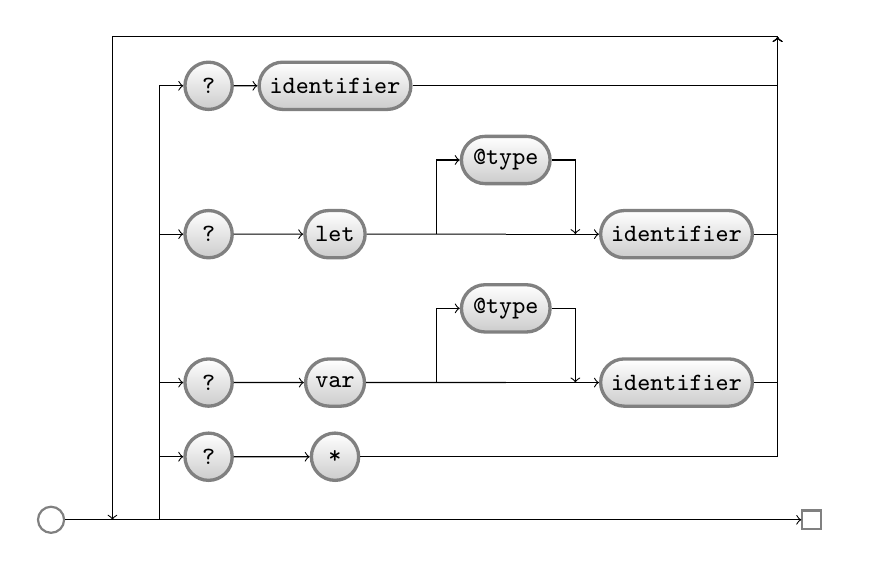
\begin{tikzpicture}
  \matrix[column sep=\ruleMatrixColumnSeparation, row sep=\ruleMatrixRowSeparation] {
    & & & & & & & & & & & \node (p7-11) [point] {}; & \\
    & & & & & \node (p6-5) [terminal] {?}; & \node (p6-6) [terminal] {identifier}; & \\
    & & & & & & & & \node (p5-8) [terminal] {@type}; & \\
    & & & & & \node (p4-5) [terminal] {?}; & \node (p4-6) [terminal] {let}; & \node (p4-7) [point] {}; & \node (p4-8) [point] {}; & \node (p4-9) [point] {}; & \node (p4-10) [terminal] {identifier}; & \\
    & & & & & & & & \node (p3-8) [terminal] {@type}; & \\
    & & & & & \node (p2-5) [terminal] {?}; & \node (p2-6) [terminal] {var}; & \node (p2-7) [point] {}; & \node (p2-8) [point] {}; & \node (p2-9) [point] {}; & \node (p2-10) [terminal] {identifier}; & \\
    & & & & & \node (p1-5) [terminal] {?}; & \node (p1-6) [terminal] {*}; & \\
    \node (P0start) [firstPoint] {}; & & \node (p0-2) [point] {}; & \node (p0-3) [point] {}; & \node (p0-4) [point] {}; & & & & & & & & \node (p0-12) [lastPoint] {}; & \\
  };
  \draw (P0start) -- (p0-3) ;
  \draw[->] (p0-4) |- (p1-5) ;
  \draw[->] (p1-5) -- (p1-6) ;
  \draw[->] (p0-4) |- (p2-5) ;
  \draw[->] (p2-5) -- (p2-6) ;
  \draw (p2-6) -- (p2-8) ;
  \draw[->] (p2-7) |- (p3-8) ;
  \draw (p2-8) -- (p2-9) ;
  \draw[->] (p3-8) -| (p2-9) ;
  \draw[->] (p2-9) -- (p2-10) ;
  \draw[->] (p0-4) |- (p4-5) ;
  \draw[->] (p4-5) -- (p4-6) ;
  \draw (p4-6) -- (p4-8) ;
  \draw[->] (p4-7) |- (p5-8) ;
  \draw (p4-8) -- (p4-9) ;
  \draw[->] (p5-8) -| (p4-9) ;
  \draw[->] (p4-9) -- (p4-10) ;
  \draw[->] (p0-4) |- (p6-5) ;
  \draw[->] (p6-5) -- (p6-6) ;
  \draw[->] (p7-11) -| (p0-2) ;
  \draw[->] (p1-6) -| (p7-11) ;
  \draw[->] (p2-10) -| (p7-11) ;
  \draw[->] (p4-10) -| (p7-11) ;
  \draw[->] (p6-6) -| (p7-11) ;
  \draw[->] (p0-3) -- (p0-12) ;
\end{tikzpicture}

\nonTerminalSection{actual\_parameter\_list}{13}

\ruleSubsection{galgas4ParameterArgumentSyntax}{galgasParameterArgumentSyntax}{317}

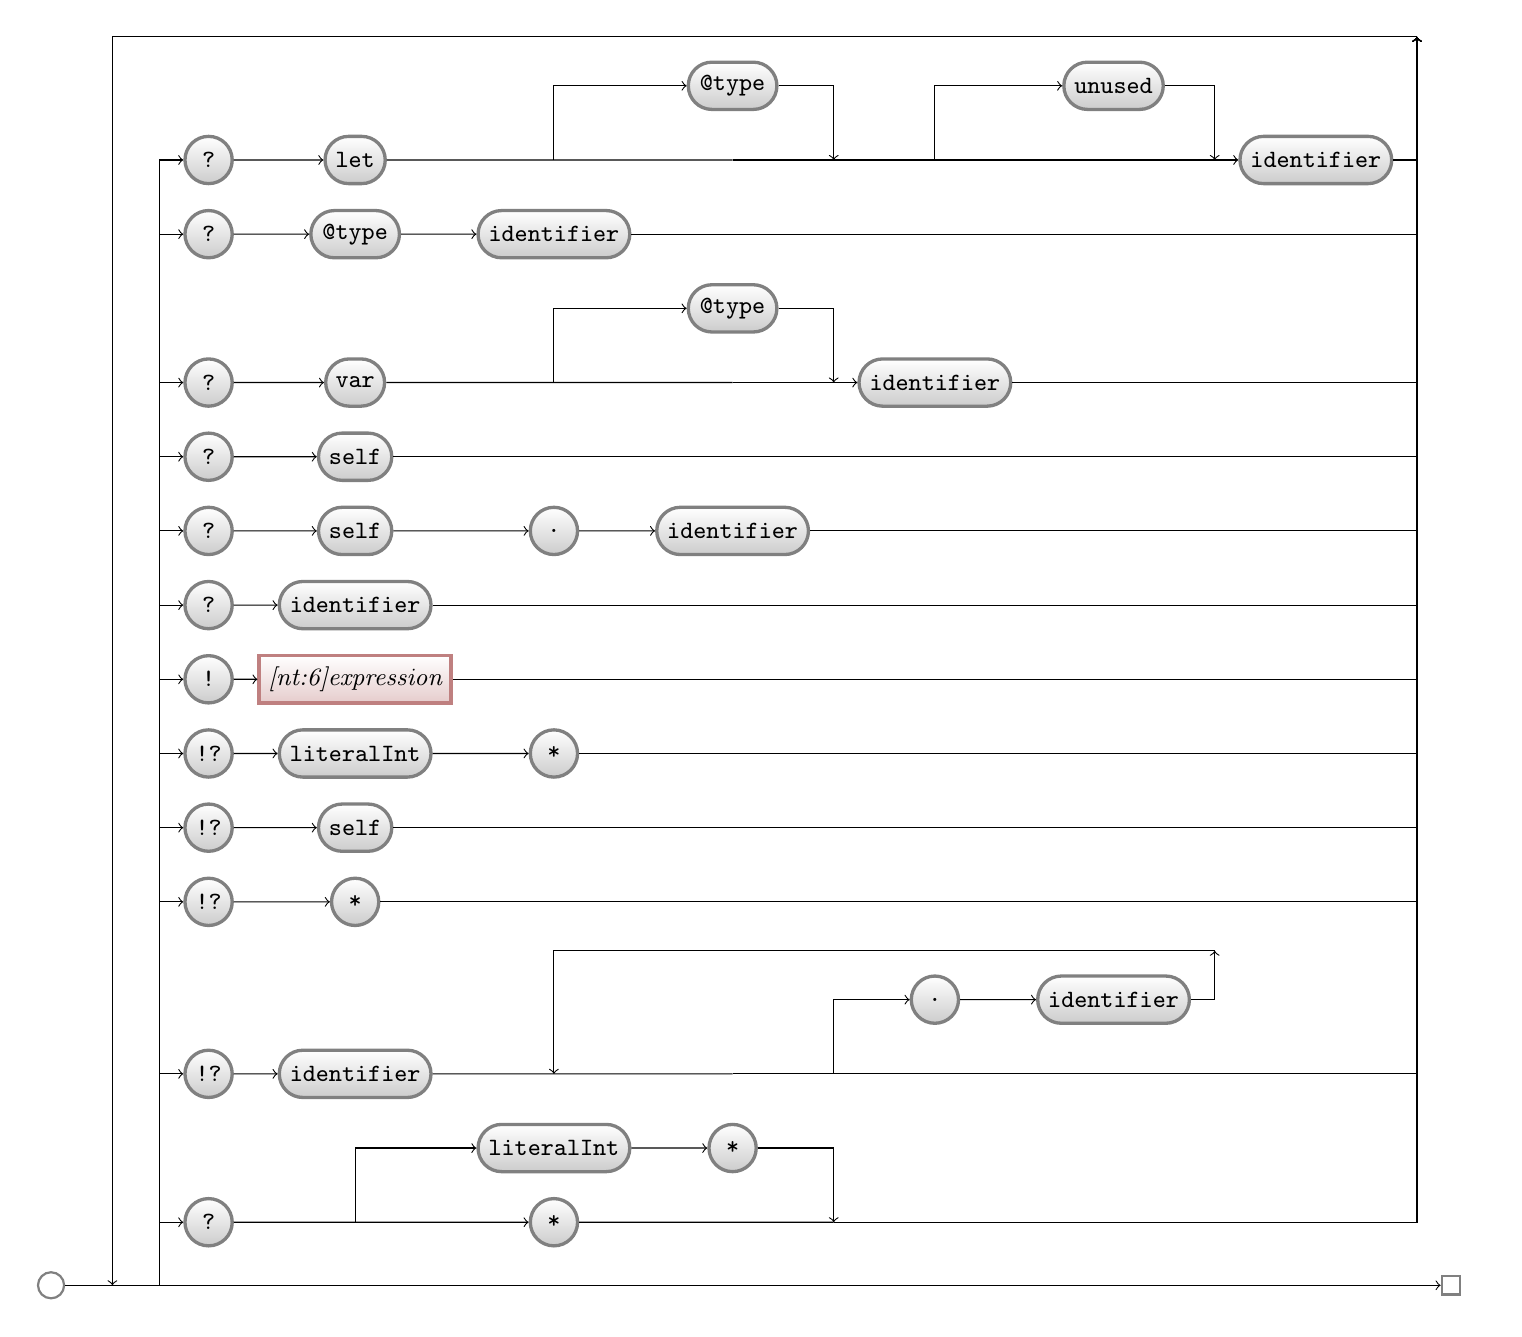
\begin{tikzpicture}
  \matrix[column sep=\ruleMatrixColumnSeparation, row sep=\ruleMatrixRowSeparation] {
    & & & & & & & & & & & & & & \node (p18-14) [point] {}; & \\
    & & & & & & & & \node (p17-8) [terminal] {@type}; & & & \node (p17-11) [terminal] {unused}; & \\
    & & & & & \node (p16-5) [terminal] {?}; & \node (p16-6) [terminal] {let}; & \node (p16-7) [point] {}; & \node (p16-8) [point] {}; & \node (p16-9) [point] {}; & \node (p16-10) [point] {}; & \node (p16-11) [point] {}; & \node (p16-12) [point] {}; & \node (p16-13) [terminal] {identifier}; & \\
    & & & & & \node (p15-5) [terminal] {?}; & \node (p15-6) [terminal] {@type}; & \node (p15-7) [terminal] {identifier}; & \\
    & & & & & & & & \node (p14-8) [terminal] {@type}; & \\
    & & & & & \node (p13-5) [terminal] {?}; & \node (p13-6) [terminal] {var}; & \node (p13-7) [point] {}; & \node (p13-8) [point] {}; & \node (p13-9) [point] {}; & \node (p13-10) [terminal] {identifier}; & \\
    & & & & & \node (p12-5) [terminal] {?}; & \node (p12-6) [terminal] {self}; & \\
    & & & & & \node (p11-5) [terminal] {?}; & \node (p11-6) [terminal] {self}; & \node (p11-7) [terminal] {.}; & \node (p11-8) [terminal] {identifier}; & \\
    & & & & & \node (p10-5) [terminal] {?}; & \node (p10-6) [terminal] {identifier}; & \\
    & & & & & \node (p9-5) [terminal] {!}; & \node (p9-6) [nonterminal] {\nonTerminalSymbol{expression}{6}}; & \\
    & & & & & \node (p8-5) [terminal] {!?}; & \node (p8-6) [terminal] {literalInt}; & \node (p8-7) [terminal] {*}; & \\
    & & & & & \node (p7-5) [terminal] {!?}; & \node (p7-6) [terminal] {self}; & \\
    & & & & & \node (p6-5) [terminal] {!?}; & \node (p6-6) [terminal] {*}; & \\
    & & & & & & & & & & & & \node (p5-12) [point] {}; & \\
    & & & & & & & & & & \node (p4-10) [terminal] {.}; & \node (p4-11) [terminal] {identifier}; & \\
    & & & & & \node (p3-5) [terminal] {!?}; & \node (p3-6) [terminal] {identifier}; & \node (p3-7) [point] {}; & \node (p3-8) [point] {}; & \node (p3-9) [point] {}; & \\
    & & & & & & & \node (p2-7) [terminal] {literalInt}; & \node (p2-8) [terminal] {*}; & \\
    & & & & & \node (p1-5) [terminal] {?}; & \node (p1-6) [point] {}; & \node (p1-7) [terminal] {*}; & & \node (p1-9) [point] {}; & \\
    \node (P0start) [firstPoint] {}; & & \node (p0-2) [point] {}; & \node (p0-3) [point] {}; & \node (p0-4) [point] {}; & & & & & & & & & & & \node (p0-15) [lastPoint] {}; & \\
  };
  \draw (P0start) -- (p0-3) ;
  \draw[->] (p0-4) |- (p1-5) ;
  \draw[->] (p1-5) -- (p1-7) ;
  \draw[->] (p1-6) |- (p2-7) ;
  \draw[->] (p2-7) -- (p2-8) ;
  \draw (p1-7) -- (p1-9) ;
  \draw[->] (p2-8) -| (p1-9) ;
  \draw[->] (p0-4) |- (p3-5) ;
  \draw[->] (p3-5) -- (p3-6) ;
  \draw (p3-6) -- (p3-8) ;
  \draw[->] (p3-9) |- (p4-10) ;
  \draw[->] (p4-10) -- (p4-11) ;
  \draw[->] (p5-12) -| (p3-7) ;
  \draw[->] (p4-11) -| (p5-12) ;
  \draw[->] (p0-4) |- (p6-5) ;
  \draw[->] (p6-5) -- (p6-6) ;
  \draw[->] (p0-4) |- (p7-5) ;
  \draw[->] (p7-5) -- (p7-6) ;
  \draw[->] (p0-4) |- (p8-5) ;
  \draw[->] (p8-5) -- (p8-6) ;
  \draw[->] (p8-6) -- (p8-7) ;
  \draw[->] (p0-4) |- (p9-5) ;
  \draw[->] (p9-5) -- (p9-6) ;
  \draw[->] (p0-4) |- (p10-5) ;
  \draw[->] (p10-5) -- (p10-6) ;
  \draw[->] (p0-4) |- (p11-5) ;
  \draw[->] (p11-5) -- (p11-6) ;
  \draw[->] (p11-6) -- (p11-7) ;
  \draw[->] (p11-7) -- (p11-8) ;
  \draw[->] (p0-4) |- (p12-5) ;
  \draw[->] (p12-5) -- (p12-6) ;
  \draw[->] (p0-4) |- (p13-5) ;
  \draw[->] (p13-5) -- (p13-6) ;
  \draw (p13-6) -- (p13-8) ;
  \draw[->] (p13-7) |- (p14-8) ;
  \draw (p13-8) -- (p13-9) ;
  \draw[->] (p14-8) -| (p13-9) ;
  \draw[->] (p13-9) -- (p13-10) ;
  \draw[->] (p0-4) |- (p15-5) ;
  \draw[->] (p15-5) -- (p15-6) ;
  \draw[->] (p15-6) -- (p15-7) ;
  \draw[->] (p0-4) |- (p16-5) ;
  \draw[->] (p16-5) -- (p16-6) ;
  \draw (p16-6) -- (p16-8) ;
  \draw[->] (p16-7) |- (p17-8) ;
  \draw (p16-8) -- (p16-9) ;
  \draw[->] (p17-8) -| (p16-9) ;
  \draw (p16-9) -- (p16-11) ;
  \draw[->] (p16-10) |- (p17-11) ;
  \draw (p16-11) -- (p16-12) ;
  \draw[->] (p17-11) -| (p16-12) ;
  \draw[->] (p16-12) -- (p16-13) ;
  \draw[->] (p18-14) -| (p0-2) ;
  \draw[->] (p1-9) -| (p18-14) ;
  \draw[->] (p3-8) -| (p18-14) ;
  \draw[->] (p6-6) -| (p18-14) ;
  \draw[->] (p7-6) -| (p18-14) ;
  \draw[->] (p8-7) -| (p18-14) ;
  \draw[->] (p9-6) -| (p18-14) ;
  \draw[->] (p10-6) -| (p18-14) ;
  \draw[->] (p11-8) -| (p18-14) ;
  \draw[->] (p12-6) -| (p18-14) ;
  \draw[->] (p13-10) -| (p18-14) ;
  \draw[->] (p15-7) -| (p18-14) ;
  \draw[->] (p16-13) -| (p18-14) ;
  \draw[->] (p0-3) -- (p0-15) ;
\end{tikzpicture}

\nonTerminalSection{actual\_parameter\_list\_within\_parenthesis}{12}

\ruleSubsection{galgas4ParameterArgumentSyntax}{galgasParameterArgumentSyntax}{309}

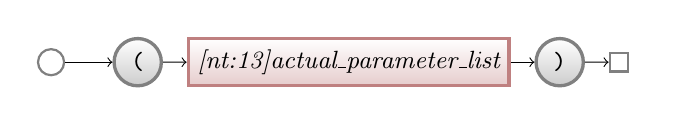
\begin{tikzpicture}
  \matrix[column sep=\ruleMatrixColumnSeparation, row sep=\ruleMatrixRowSeparation] {
    \node (P0start) [firstPoint] {}; & & \node (p0-2) [terminal] {(}; & \node (p0-3) [nonterminal] {\nonTerminalSymbol{actual\_parameter\_list}{13}}; & \node (p0-4) [terminal] {)}; & \node (p0-5) [lastPoint] {}; & \\
  };
  \draw[->] (P0start) -- (p0-2) ;
  \draw[->] (p0-2) -- (p0-3) ;
  \draw[->] (p0-3) -- (p0-4) ;
  \draw[->] (p0-4) -- (p0-5) ;
\end{tikzpicture}

\nonTerminalSection{branchOfParseWhithInstruction}{75}

\ruleSubsection{galgas4SyntaxComponentSyntax}{instruction-parse-when}{95}

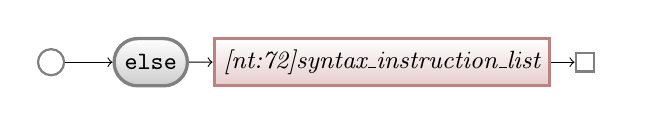
\begin{tikzpicture}
  \matrix[column sep=\ruleMatrixColumnSeparation, row sep=\ruleMatrixRowSeparation] {
    \node (P0start) [firstPoint] {}; & & \node (p0-2) [terminal] {else}; & \node (p0-3) [nonterminal] {\nonTerminalSymbol{syntax\_instruction\_list}{72}}; & \node (p0-4) [lastPoint] {}; & \\
  };
  \draw[->] (P0start) -- (p0-2) ;
  \draw[->] (p0-2) -- (p0-3) ;
  \draw[->] (p0-3) -- (p0-4) ;
\end{tikzpicture}

\ruleSubsection{galgas4SyntaxComponentSyntax}{instruction-parse-when}{102}

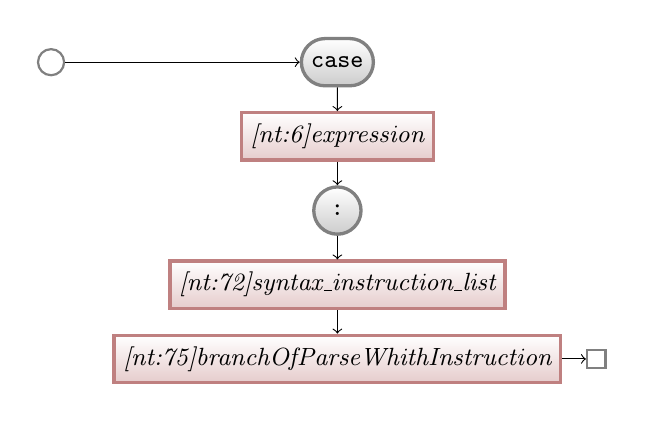
\begin{tikzpicture}
  \matrix[column sep=\ruleMatrixColumnSeparation, row sep=\ruleMatrixRowSeparation] {
    \node (P0start) [firstPoint] {}; & & \node (p4-2) [terminal] {case}; & \\
    & & \node (p3-2) [nonterminal] {\nonTerminalSymbol{expression}{6}}; & \\
    & & \node (p2-2) [terminal] {:}; & \\
    & & \node (p1-2) [nonterminal] {\nonTerminalSymbol{syntax\_instruction\_list}{72}}; & \\
    & & \node (p0-2) [nonterminal] {\nonTerminalSymbol{branchOfParseWhithInstruction}{75}}; & \node (p0-3) [lastPoint] {}; & \\
  };
  \draw[->] (P0start) -- (p4-2) ;
  \draw[->] (p4-2) -- (p3-2) ;
  \draw[->] (p3-2) -- (p2-2) ;
  \draw[->] (p2-2) -- (p1-2) ;
  \draw[->] (p1-2) -- (p0-2) ;
  \draw[->] (p0-2) -- (p0-3) ;
\end{tikzpicture}

\nonTerminalSection{collection\_value\_element}{8}

\ruleSubsection{galgas4ExpressionSyntax}{expression-collection-value}{117}

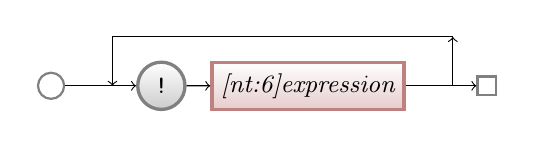
\begin{tikzpicture}
  \matrix[column sep=\ruleMatrixColumnSeparation, row sep=\ruleMatrixRowSeparation] {
    & & & & & & \node (p1-6) [point] {}; & \\
    \node (P0start) [firstPoint] {}; & & \node (p0-2) [point] {}; & \node (p0-3) [terminal] {!}; & \node (p0-4) [nonterminal] {\nonTerminalSymbol{expression}{6}}; & \node (p0-5) [point] {}; & & \node (p0-7) [lastPoint] {}; & \\
  };
  \draw[->] (P0start) -- (p0-3) ;
  \draw[->] (p0-3) -- (p0-4) ;
  \draw[->] (p1-6) -| (p0-2) ;
  \draw[->] (p0-5) -| (p1-6) ;
  \draw[->] (p0-4) -- (p0-7) ;
\end{tikzpicture}

\ruleSubsection{galgas4ExpressionSyntax}{expression-collection-value}{130}

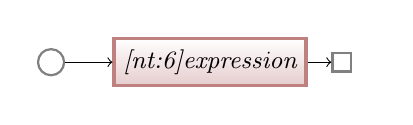
\begin{tikzpicture}
  \matrix[column sep=\ruleMatrixColumnSeparation, row sep=\ruleMatrixRowSeparation] {
    \node (P0start) [firstPoint] {}; & & \node (p0-2) [nonterminal] {\nonTerminalSymbol{expression}{6}}; & \node (p0-3) [lastPoint] {}; & \\
  };
  \draw[->] (P0start) -- (p0-2) ;
  \draw[->] (p0-2) -- (p0-3) ;
\end{tikzpicture}

\nonTerminalSection{declaration}{17}

\ruleSubsection{galgas4InstructionsSyntax}{galgasInstructionsSyntax}{370}

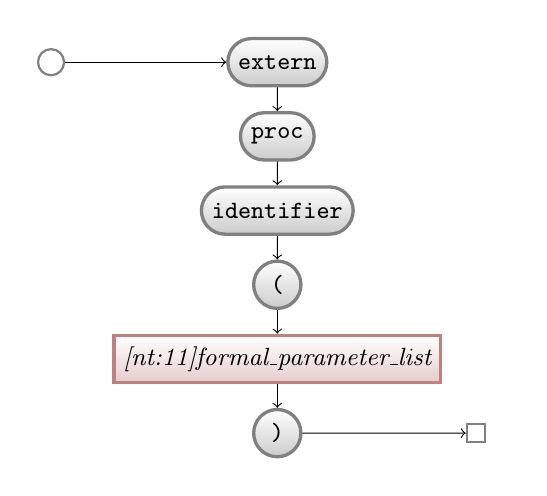
\begin{tikzpicture}
  \matrix[column sep=\ruleMatrixColumnSeparation, row sep=\ruleMatrixRowSeparation] {
    \node (P0start) [firstPoint] {}; & & \node (p5-2) [terminal] {extern}; & \\
    & & \node (p4-2) [terminal] {proc}; & \\
    & & \node (p3-2) [terminal] {identifier}; & \\
    & & \node (p2-2) [terminal] {(}; & \\
    & & \node (p1-2) [nonterminal] {\nonTerminalSymbol{formal\_parameter\_list}{11}}; & \\
    & & \node (p0-2) [terminal] {)}; & \node (p0-3) [lastPoint] {}; & \\
  };
  \draw[->] (P0start) -- (p5-2) ;
  \draw[->] (p5-2) -- (p4-2) ;
  \draw[->] (p4-2) -- (p3-2) ;
  \draw[->] (p3-2) -- (p2-2) ;
  \draw[->] (p2-2) -- (p1-2) ;
  \draw[->] (p1-2) -- (p0-2) ;
  \draw[->] (p0-2) -- (p0-3) ;
\end{tikzpicture}

\ruleSubsection{galgas4InstructionsSyntax}{galgasInstructionsSyntax}{389}

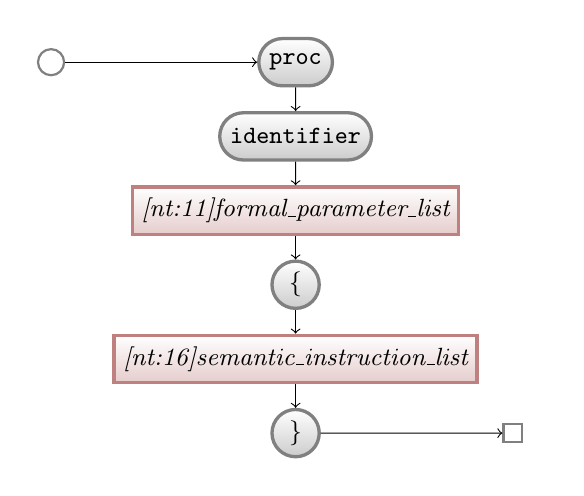
\begin{tikzpicture}
  \matrix[column sep=\ruleMatrixColumnSeparation, row sep=\ruleMatrixRowSeparation] {
    \node (P0start) [firstPoint] {}; & & \node (p5-2) [terminal] {proc}; & \\
    & & \node (p4-2) [terminal] {identifier}; & \\
    & & \node (p3-2) [nonterminal] {\nonTerminalSymbol{formal\_parameter\_list}{11}}; & \\
    & & \node (p2-2) [terminal] {\{}; & \\
    & & \node (p1-2) [nonterminal] {\nonTerminalSymbol{semantic\_instruction\_list}{16}}; & \\
    & & \node (p0-2) [terminal] {\}}; & \node (p0-3) [lastPoint] {}; & \\
  };
  \draw[->] (P0start) -- (p5-2) ;
  \draw[->] (p5-2) -- (p4-2) ;
  \draw[->] (p4-2) -- (p3-2) ;
  \draw[->] (p3-2) -- (p2-2) ;
  \draw[->] (p2-2) -- (p1-2) ;
  \draw[->] (p1-2) -- (p0-2) ;
  \draw[->] (p0-2) -- (p0-3) ;
\end{tikzpicture}

\ruleSubsection{galgas4InstructionsSyntax}{galgasInstructionsSyntax}{409}

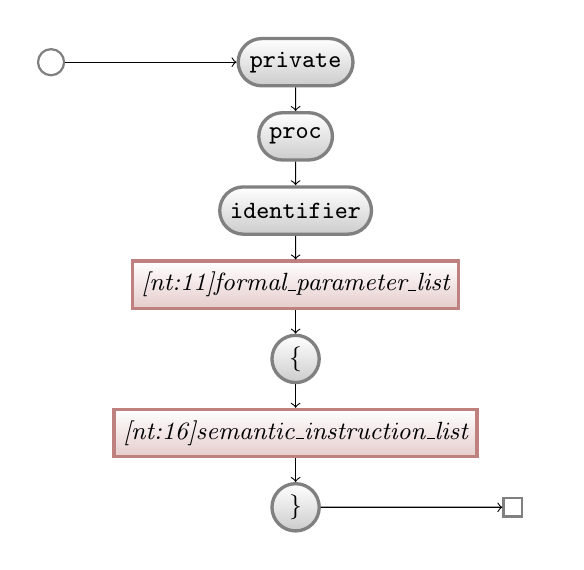
\begin{tikzpicture}
  \matrix[column sep=\ruleMatrixColumnSeparation, row sep=\ruleMatrixRowSeparation] {
    \node (P0start) [firstPoint] {}; & & \node (p6-2) [terminal] {private}; & \\
    & & \node (p5-2) [terminal] {proc}; & \\
    & & \node (p4-2) [terminal] {identifier}; & \\
    & & \node (p3-2) [nonterminal] {\nonTerminalSymbol{formal\_parameter\_list}{11}}; & \\
    & & \node (p2-2) [terminal] {\{}; & \\
    & & \node (p1-2) [nonterminal] {\nonTerminalSymbol{semantic\_instruction\_list}{16}}; & \\
    & & \node (p0-2) [terminal] {\}}; & \node (p0-3) [lastPoint] {}; & \\
  };
  \draw[->] (P0start) -- (p6-2) ;
  \draw[->] (p6-2) -- (p5-2) ;
  \draw[->] (p5-2) -- (p4-2) ;
  \draw[->] (p4-2) -- (p3-2) ;
  \draw[->] (p3-2) -- (p2-2) ;
  \draw[->] (p2-2) -- (p1-2) ;
  \draw[->] (p1-2) -- (p0-2) ;
  \draw[->] (p0-2) -- (p0-3) ;
\end{tikzpicture}

\ruleSubsection{galgas4InstructionsSyntax}{galgasInstructionsSyntax}{432}

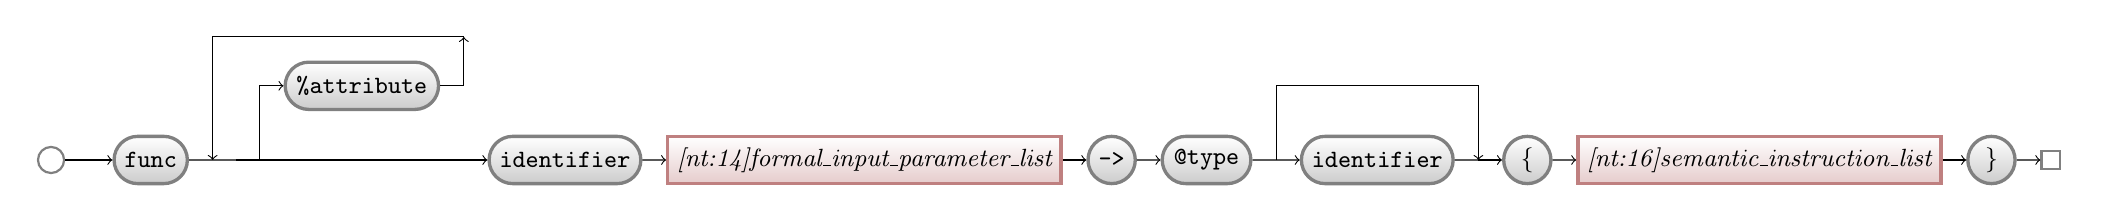
\begin{tikzpicture}
  \matrix[column sep=\ruleMatrixColumnSeparation, row sep=\ruleMatrixRowSeparation] {
    & & & & & & & \node (p2-7) [point] {}; & \\
    & & & & & & \node (p1-6) [terminal] {\verb=%=attribute}; & & & & & & & \node (p1-13) [point] {}; & \\
    \node (P0start) [firstPoint] {}; & & \node (p0-2) [terminal] {func}; & \node (p0-3) [point] {}; & \node (p0-4) [point] {}; & \node (p0-5) [point] {}; & & & \node (p0-8) [terminal] {identifier}; & \node (p0-9) [nonterminal] {\nonTerminalSymbol{formal\_input\_parameter\_list}{14}}; & \node (p0-10) [terminal] {->}; & \node (p0-11) [terminal] {@type}; & \node (p0-12) [point] {}; & \node (p0-13) [terminal] {identifier}; & \node (p0-14) [point] {}; & \node (p0-15) [terminal] {\{}; & \node (p0-16) [nonterminal] {\nonTerminalSymbol{semantic\_instruction\_list}{16}}; & \node (p0-17) [terminal] {\}}; & \node (p0-18) [lastPoint] {}; & \\
  };
  \draw[->] (P0start) -- (p0-2) ;
  \draw (p0-2) -- (p0-4) ;
  \draw[->] (p0-5) |- (p1-6) ;
  \draw[->] (p2-7) -| (p0-3) ;
  \draw[->] (p1-6) -| (p2-7) ;
  \draw[->] (p0-4) -- (p0-8) ;
  \draw[->] (p0-8) -- (p0-9) ;
  \draw[->] (p0-9) -- (p0-10) ;
  \draw[->] (p0-10) -- (p0-11) ;
  \draw[->] (p0-11) -- (p0-13) ;
  \draw (p0-12) |- (p1-13) ;
  \draw (p0-13) -- (p0-14) ;
  \draw[->] (p1-13) -| (p0-14) ;
  \draw[->] (p0-14) -- (p0-15) ;
  \draw[->] (p0-15) -- (p0-16) ;
  \draw[->] (p0-16) -- (p0-17) ;
  \draw[->] (p0-17) -- (p0-18) ;
\end{tikzpicture}

\ruleSubsection{galgas4InstructionsSyntax}{galgasInstructionsSyntax}{498}

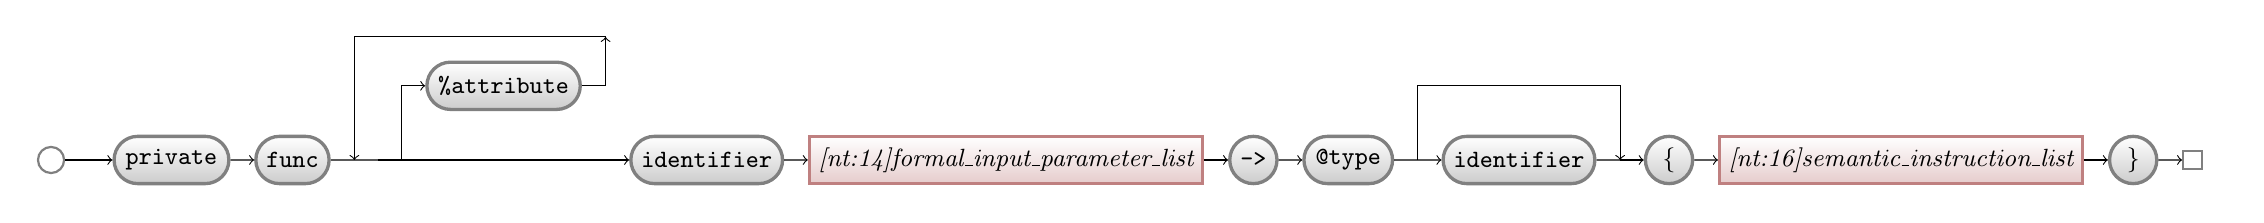
\begin{tikzpicture}
  \matrix[column sep=\ruleMatrixColumnSeparation, row sep=\ruleMatrixRowSeparation] {
    & & & & & & & & \node (p2-8) [point] {}; & \\
    & & & & & & & \node (p1-7) [terminal] {\verb=%=attribute}; & & & & & & & \node (p1-14) [point] {}; & \\
    \node (P0start) [firstPoint] {}; & & \node (p0-2) [terminal] {private}; & \node (p0-3) [terminal] {func}; & \node (p0-4) [point] {}; & \node (p0-5) [point] {}; & \node (p0-6) [point] {}; & & & \node (p0-9) [terminal] {identifier}; & \node (p0-10) [nonterminal] {\nonTerminalSymbol{formal\_input\_parameter\_list}{14}}; & \node (p0-11) [terminal] {->}; & \node (p0-12) [terminal] {@type}; & \node (p0-13) [point] {}; & \node (p0-14) [terminal] {identifier}; & \node (p0-15) [point] {}; & \node (p0-16) [terminal] {\{}; & \node (p0-17) [nonterminal] {\nonTerminalSymbol{semantic\_instruction\_list}{16}}; & \node (p0-18) [terminal] {\}}; & \node (p0-19) [lastPoint] {}; & \\
  };
  \draw[->] (P0start) -- (p0-2) ;
  \draw[->] (p0-2) -- (p0-3) ;
  \draw (p0-3) -- (p0-5) ;
  \draw[->] (p0-6) |- (p1-7) ;
  \draw[->] (p2-8) -| (p0-4) ;
  \draw[->] (p1-7) -| (p2-8) ;
  \draw[->] (p0-5) -- (p0-9) ;
  \draw[->] (p0-9) -- (p0-10) ;
  \draw[->] (p0-10) -- (p0-11) ;
  \draw[->] (p0-11) -- (p0-12) ;
  \draw[->] (p0-12) -- (p0-14) ;
  \draw (p0-13) |- (p1-14) ;
  \draw (p0-14) -- (p0-15) ;
  \draw[->] (p1-14) -| (p0-15) ;
  \draw[->] (p0-15) -- (p0-16) ;
  \draw[->] (p0-16) -- (p0-17) ;
  \draw[->] (p0-17) -- (p0-18) ;
  \draw[->] (p0-18) -- (p0-19) ;
\end{tikzpicture}

\ruleSubsection{galgas4InstructionsSyntax}{galgasInstructionsSyntax}{567}

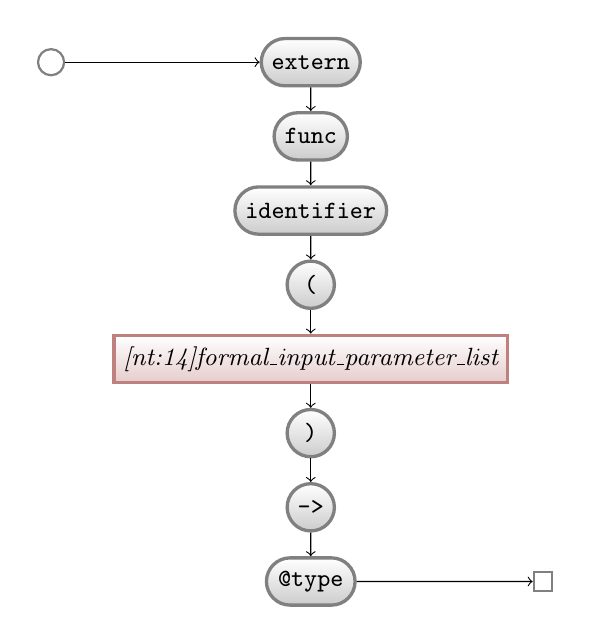
\begin{tikzpicture}
  \matrix[column sep=\ruleMatrixColumnSeparation, row sep=\ruleMatrixRowSeparation] {
    \node (P0start) [firstPoint] {}; & & \node (p7-2) [terminal] {extern}; & \\
    & & \node (p6-2) [terminal] {func}; & \\
    & & \node (p5-2) [terminal] {identifier}; & \\
    & & \node (p4-2) [terminal] {(}; & \\
    & & \node (p3-2) [nonterminal] {\nonTerminalSymbol{formal\_input\_parameter\_list}{14}}; & \\
    & & \node (p2-2) [terminal] {)}; & \\
    & & \node (p1-2) [terminal] {->}; & \\
    & & \node (p0-2) [terminal] {@type}; & \node (p0-3) [lastPoint] {}; & \\
  };
  \draw[->] (P0start) -- (p7-2) ;
  \draw[->] (p7-2) -- (p6-2) ;
  \draw[->] (p6-2) -- (p5-2) ;
  \draw[->] (p5-2) -- (p4-2) ;
  \draw[->] (p4-2) -- (p3-2) ;
  \draw[->] (p3-2) -- (p2-2) ;
  \draw[->] (p2-2) -- (p1-2) ;
  \draw[->] (p1-2) -- (p0-2) ;
  \draw[->] (p0-2) -- (p0-3) ;
\end{tikzpicture}

\ruleSubsection{galgas4DeclarationsSyntax}{galgasDeclarationsSyntax}{337}

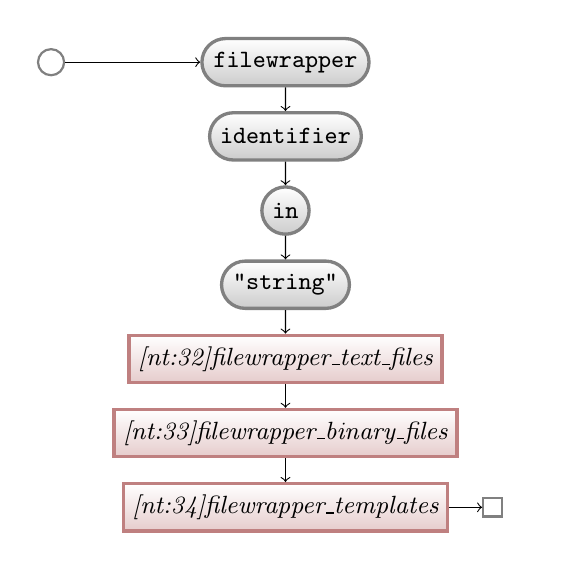
\begin{tikzpicture}
  \matrix[column sep=\ruleMatrixColumnSeparation, row sep=\ruleMatrixRowSeparation] {
    \node (P0start) [firstPoint] {}; & & \node (p6-2) [terminal] {filewrapper}; & \\
    & & \node (p5-2) [terminal] {identifier}; & \\
    & & \node (p4-2) [terminal] {in}; & \\
    & & \node (p3-2) [terminal] {"string"}; & \\
    & & \node (p2-2) [nonterminal] {\nonTerminalSymbol{filewrapper\_text\_files}{32}}; & \\
    & & \node (p1-2) [nonterminal] {\nonTerminalSymbol{filewrapper\_binary\_files}{33}}; & \\
    & & \node (p0-2) [nonterminal] {\nonTerminalSymbol{filewrapper\_templates}{34}}; & \node (p0-3) [lastPoint] {}; & \\
  };
  \draw[->] (P0start) -- (p6-2) ;
  \draw[->] (p6-2) -- (p5-2) ;
  \draw[->] (p5-2) -- (p4-2) ;
  \draw[->] (p4-2) -- (p3-2) ;
  \draw[->] (p3-2) -- (p2-2) ;
  \draw[->] (p2-2) -- (p1-2) ;
  \draw[->] (p1-2) -- (p0-2) ;
  \draw[->] (p0-2) -- (p0-3) ;
\end{tikzpicture}

\ruleSubsection{galgas4DeclarationsSyntax}{galgasDeclarationsSyntax}{358}

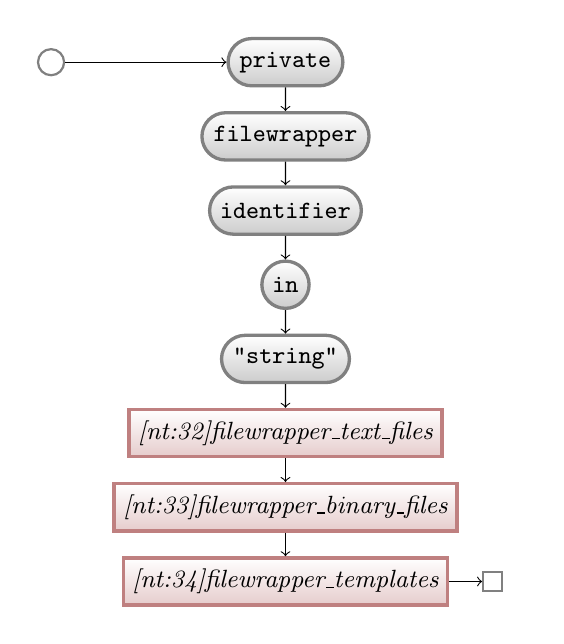
\begin{tikzpicture}
  \matrix[column sep=\ruleMatrixColumnSeparation, row sep=\ruleMatrixRowSeparation] {
    \node (P0start) [firstPoint] {}; & & \node (p7-2) [terminal] {private}; & \\
    & & \node (p6-2) [terminal] {filewrapper}; & \\
    & & \node (p5-2) [terminal] {identifier}; & \\
    & & \node (p4-2) [terminal] {in}; & \\
    & & \node (p3-2) [terminal] {"string"}; & \\
    & & \node (p2-2) [nonterminal] {\nonTerminalSymbol{filewrapper\_text\_files}{32}}; & \\
    & & \node (p1-2) [nonterminal] {\nonTerminalSymbol{filewrapper\_binary\_files}{33}}; & \\
    & & \node (p0-2) [nonterminal] {\nonTerminalSymbol{filewrapper\_templates}{34}}; & \node (p0-3) [lastPoint] {}; & \\
  };
  \draw[->] (P0start) -- (p7-2) ;
  \draw[->] (p7-2) -- (p6-2) ;
  \draw[->] (p6-2) -- (p5-2) ;
  \draw[->] (p5-2) -- (p4-2) ;
  \draw[->] (p4-2) -- (p3-2) ;
  \draw[->] (p3-2) -- (p2-2) ;
  \draw[->] (p2-2) -- (p1-2) ;
  \draw[->] (p1-2) -- (p0-2) ;
  \draw[->] (p0-2) -- (p0-3) ;
\end{tikzpicture}

\ruleSubsection{galgas4DeclarationsSyntax}{type-array}{46}

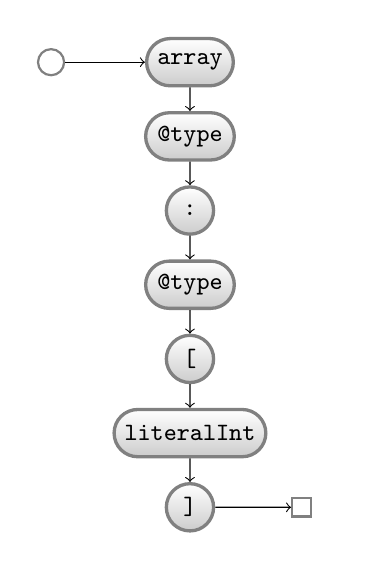
\begin{tikzpicture}
  \matrix[column sep=\ruleMatrixColumnSeparation, row sep=\ruleMatrixRowSeparation] {
    \node (P0start) [firstPoint] {}; & & \node (p6-2) [terminal] {array}; & \\
    & & \node (p5-2) [terminal] {@type}; & \\
    & & \node (p4-2) [terminal] {:}; & \\
    & & \node (p3-2) [terminal] {@type}; & \\
    & & \node (p2-2) [terminal] {[}; & \\
    & & \node (p1-2) [terminal] {literalInt}; & \\
    & & \node (p0-2) [terminal] {]}; & \node (p0-3) [lastPoint] {}; & \\
  };
  \draw[->] (P0start) -- (p6-2) ;
  \draw[->] (p6-2) -- (p5-2) ;
  \draw[->] (p5-2) -- (p4-2) ;
  \draw[->] (p4-2) -- (p3-2) ;
  \draw[->] (p3-2) -- (p2-2) ;
  \draw[->] (p2-2) -- (p1-2) ;
  \draw[->] (p1-2) -- (p0-2) ;
  \draw[->] (p0-2) -- (p0-3) ;
\end{tikzpicture}

\ruleSubsection{galgas4DeclarationsSyntax}{type-boolset}{47}

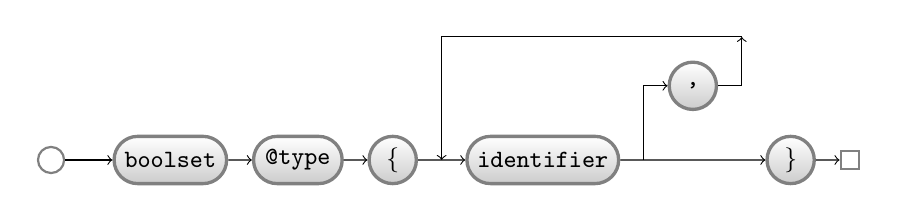
\begin{tikzpicture}
  \matrix[column sep=\ruleMatrixColumnSeparation, row sep=\ruleMatrixRowSeparation] {
    & & & & & & & & & \node (p2-9) [point] {}; & \\
    & & & & & & & & \node (p1-8) [terminal] {,}; & \\
    \node (P0start) [firstPoint] {}; & & \node (p0-2) [terminal] {boolset}; & \node (p0-3) [terminal] {@type}; & \node (p0-4) [terminal] {\{}; & \node (p0-5) [point] {}; & \node (p0-6) [terminal] {identifier}; & \node (p0-7) [point] {}; & & & \node (p0-10) [terminal] {\}}; & \node (p0-11) [lastPoint] {}; & \\
  };
  \draw[->] (P0start) -- (p0-2) ;
  \draw[->] (p0-2) -- (p0-3) ;
  \draw[->] (p0-3) -- (p0-4) ;
  \draw[->] (p0-4) -- (p0-6) ;
  \draw[->] (p0-7) |- (p1-8) ;
  \draw[->] (p2-9) -| (p0-5) ;
  \draw[->] (p1-8) -| (p2-9) ;
  \draw[->] (p0-6) -- (p0-10) ;
  \draw[->] (p0-10) -- (p0-11) ;
\end{tikzpicture}

\ruleSubsection{galgas4DeclarationsSyntax}{type-class}{111}

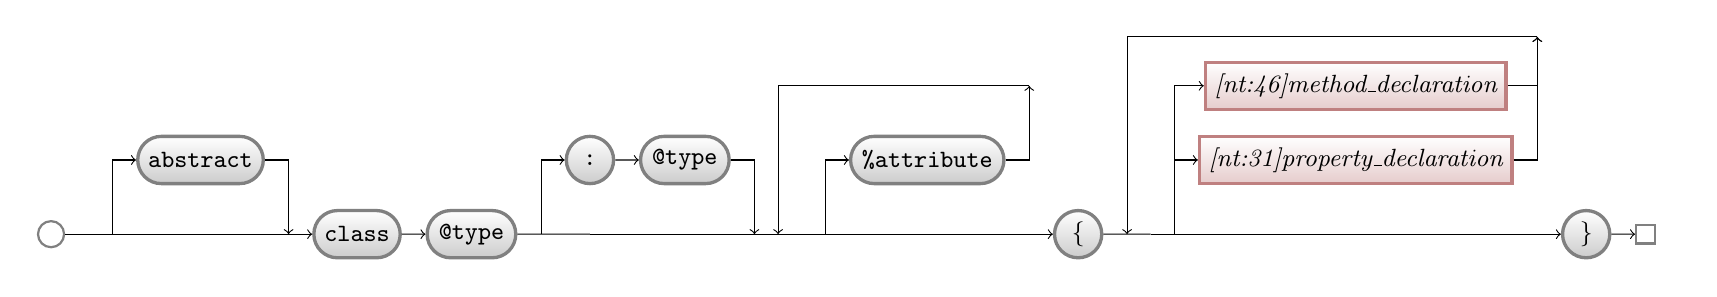
\begin{tikzpicture}
  \matrix[column sep=\ruleMatrixColumnSeparation, row sep=\ruleMatrixRowSeparation] {
    & & & & & & & & & & & & & & & & & & & & & \node (p3-21) [point] {}; & \\
    & & & & & & & & & & & & & & & \node (p2-15) [point] {}; & & & & & \node (p2-20) [nonterminal] {\nonTerminalSymbol{method\_declaration}{46}}; & \\
    & & & \node (p1-3) [terminal] {abstract}; & & & & & \node (p1-8) [terminal] {:}; & \node (p1-9) [terminal] {@type}; & & & & & \node (p1-14) [terminal] {\verb=%=attribute}; & & & & & & \node (p1-20) [nonterminal] {\nonTerminalSymbol{property\_declaration}{31}}; & \\
    \node (P0start) [firstPoint] {}; & & \node (p0-2) [point] {}; & \node (p0-3) [point] {}; & \node (p0-4) [point] {}; & \node (p0-5) [terminal] {class}; & \node (p0-6) [terminal] {@type}; & \node (p0-7) [point] {}; & \node (p0-8) [point] {}; & & \node (p0-10) [point] {}; & \node (p0-11) [point] {}; & \node (p0-12) [point] {}; & \node (p0-13) [point] {}; & & & \node (p0-16) [terminal] {\{}; & \node (p0-17) [point] {}; & \node (p0-18) [point] {}; & \node (p0-19) [point] {}; & & & \node (p0-22) [terminal] {\}}; & \node (p0-23) [lastPoint] {}; & \\
  };
  \draw (P0start) -- (p0-3) ;
  \draw[->] (p0-2) |- (p1-3) ;
  \draw (p0-3) -- (p0-4) ;
  \draw[->] (p1-3) -| (p0-4) ;
  \draw[->] (p0-4) -- (p0-5) ;
  \draw[->] (p0-5) -- (p0-6) ;
  \draw (p0-6) -- (p0-8) ;
  \draw[->] (p0-7) |- (p1-8) ;
  \draw[->] (p1-8) -- (p1-9) ;
  \draw (p0-8) -- (p0-10) ;
  \draw[->] (p1-9) -| (p0-10) ;
  \draw (p0-10) -- (p0-12) ;
  \draw[->] (p0-13) |- (p1-14) ;
  \draw[->] (p2-15) -| (p0-11) ;
  \draw[->] (p1-14) -| (p2-15) ;
  \draw[->] (p0-12) -- (p0-16) ;
  \draw (p0-16) -- (p0-18) ;
  \draw[->] (p0-19) |- (p1-20) ;
  \draw[->] (p0-19) |- (p2-20) ;
  \draw[->] (p3-21) -| (p0-17) ;
  \draw[->] (p1-20) -| (p3-21) ;
  \draw[->] (p2-20) -| (p3-21) ;
  \draw[->] (p0-18) -- (p0-22) ;
  \draw[->] (p0-22) -- (p0-23) ;
\end{tikzpicture}

\ruleSubsection{galgas4DeclarationsSyntax}{type-enum}{75}

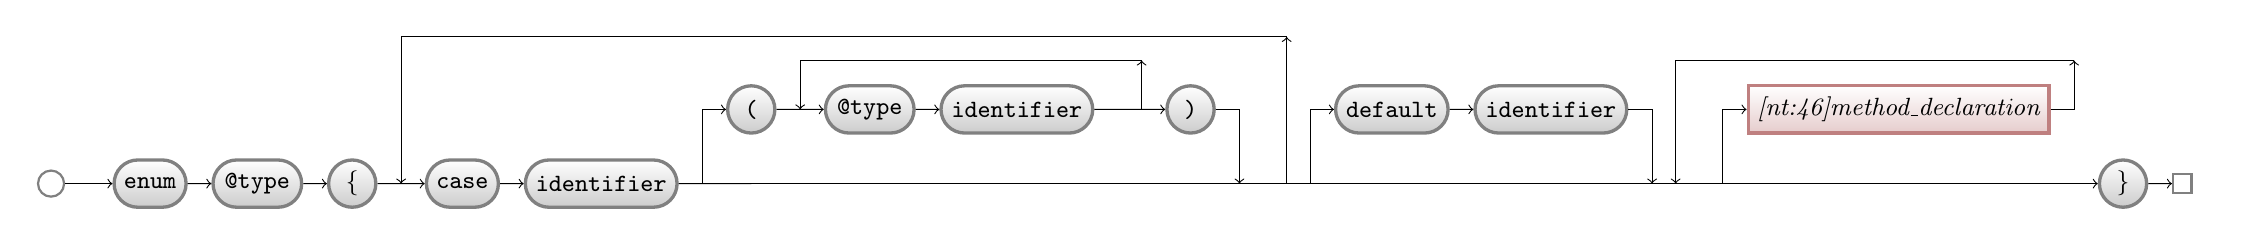
\begin{tikzpicture}
  \matrix[column sep=\ruleMatrixColumnSeparation, row sep=\ruleMatrixRowSeparation] {
    & & & & & & & & & & & & & & & & & & \node (p3-18) [point] {}; & \\
    & & & & & & & & & & & & & & \node (p2-14) [point] {}; & & & & & & & & & & & & & \node (p2-27) [point] {}; & \\
    & & & & & & & & & \node (p1-9) [terminal] {(}; & \node (p1-10) [point] {}; & \node (p1-11) [terminal] {@type}; & \node (p1-12) [terminal] {identifier}; & \node (p1-13) [point] {}; & & \node (p1-15) [terminal] {)}; & & & & & \node (p1-20) [terminal] {default}; & \node (p1-21) [terminal] {identifier}; & & & & & \node (p1-26) [nonterminal] {\nonTerminalSymbol{method\_declaration}{46}}; & \\
    \node (P0start) [firstPoint] {}; & & \node (p0-2) [terminal] {enum}; & \node (p0-3) [terminal] {@type}; & \node (p0-4) [terminal] {\{}; & \node (p0-5) [point] {}; & \node (p0-6) [terminal] {case}; & \node (p0-7) [terminal] {identifier}; & \node (p0-8) [point] {}; & \node (p0-9) [point] {}; & & & & & & & \node (p0-16) [point] {}; & \node (p0-17) [point] {}; & & \node (p0-19) [point] {}; & \node (p0-20) [point] {}; & & \node (p0-22) [point] {}; & \node (p0-23) [point] {}; & \node (p0-24) [point] {}; & \node (p0-25) [point] {}; & & & \node (p0-28) [terminal] {\}}; & \node (p0-29) [lastPoint] {}; & \\
  };
  \draw[->] (P0start) -- (p0-2) ;
  \draw[->] (p0-2) -- (p0-3) ;
  \draw[->] (p0-3) -- (p0-4) ;
  \draw[->] (p0-4) -- (p0-6) ;
  \draw[->] (p0-6) -- (p0-7) ;
  \draw (p0-7) -- (p0-9) ;
  \draw[->] (p0-8) |- (p1-9) ;
  \draw[->] (p1-9) -- (p1-11) ;
  \draw[->] (p1-11) -- (p1-12) ;
  \draw[->] (p2-14) -| (p1-10) ;
  \draw[->] (p1-13) -| (p2-14) ;
  \draw[->] (p1-12) -- (p1-15) ;
  \draw (p0-9) -- (p0-16) ;
  \draw[->] (p1-15) -| (p0-16) ;
  \draw[->] (p3-18) -| (p0-5) ;
  \draw[->] (p0-17) -| (p3-18) ;
  \draw (p0-16) -- (p0-20) ;
  \draw[->] (p0-19) |- (p1-20) ;
  \draw[->] (p1-20) -- (p1-21) ;
  \draw (p0-20) -- (p0-22) ;
  \draw[->] (p1-21) -| (p0-22) ;
  \draw (p0-22) -- (p0-24) ;
  \draw[->] (p0-25) |- (p1-26) ;
  \draw[->] (p2-27) -| (p0-23) ;
  \draw[->] (p1-26) -| (p2-27) ;
  \draw[->] (p0-24) -- (p0-28) ;
  \draw[->] (p0-28) -- (p0-29) ;
\end{tikzpicture}

\ruleSubsection{galgas4DeclarationsSyntax}{type-extern}{186}

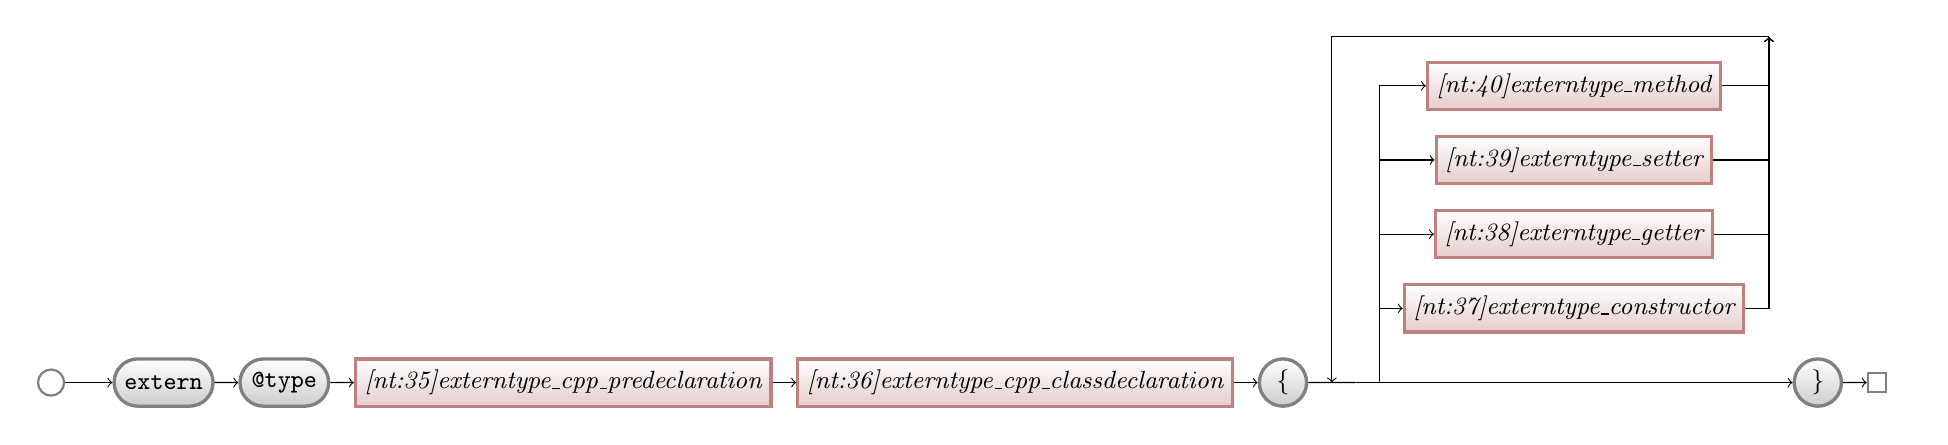
\begin{tikzpicture}
  \matrix[column sep=\ruleMatrixColumnSeparation, row sep=\ruleMatrixRowSeparation] {
    & & & & & & & & & & & \node (p5-11) [point] {}; & \\
    & & & & & & & & & & \node (p4-10) [nonterminal] {\nonTerminalSymbol{externtype\_method}{40}}; & \\
    & & & & & & & & & & \node (p3-10) [nonterminal] {\nonTerminalSymbol{externtype\_setter}{39}}; & \\
    & & & & & & & & & & \node (p2-10) [nonterminal] {\nonTerminalSymbol{externtype\_getter}{38}}; & \\
    & & & & & & & & & & \node (p1-10) [nonterminal] {\nonTerminalSymbol{externtype\_constructor}{37}}; & \\
    \node (P0start) [firstPoint] {}; & & \node (p0-2) [terminal] {extern}; & \node (p0-3) [terminal] {@type}; & \node (p0-4) [nonterminal] {\nonTerminalSymbol{externtype\_cpp\_predeclaration}{35}}; & \node (p0-5) [nonterminal] {\nonTerminalSymbol{externtype\_cpp\_classdeclaration}{36}}; & \node (p0-6) [terminal] {\{}; & \node (p0-7) [point] {}; & \node (p0-8) [point] {}; & \node (p0-9) [point] {}; & & & \node (p0-12) [terminal] {\}}; & \node (p0-13) [lastPoint] {}; & \\
  };
  \draw[->] (P0start) -- (p0-2) ;
  \draw[->] (p0-2) -- (p0-3) ;
  \draw[->] (p0-3) -- (p0-4) ;
  \draw[->] (p0-4) -- (p0-5) ;
  \draw[->] (p0-5) -- (p0-6) ;
  \draw (p0-6) -- (p0-8) ;
  \draw[->] (p0-9) |- (p1-10) ;
  \draw[->] (p0-9) |- (p2-10) ;
  \draw[->] (p0-9) |- (p3-10) ;
  \draw[->] (p0-9) |- (p4-10) ;
  \draw[->] (p5-11) -| (p0-7) ;
  \draw[->] (p1-10) -| (p5-11) ;
  \draw[->] (p2-10) -| (p5-11) ;
  \draw[->] (p3-10) -| (p5-11) ;
  \draw[->] (p4-10) -| (p5-11) ;
  \draw[->] (p0-8) -- (p0-12) ;
  \draw[->] (p0-12) -- (p0-13) ;
\end{tikzpicture}

\ruleSubsection{galgas4DeclarationsSyntax}{type-graph}{63}

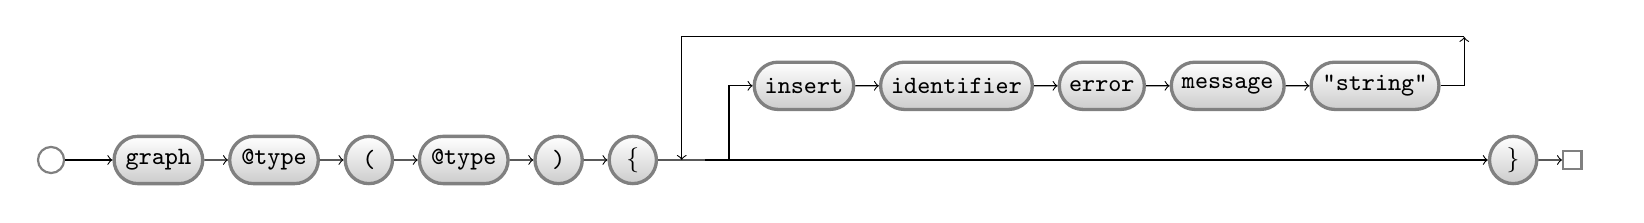
\begin{tikzpicture}
  \matrix[column sep=\ruleMatrixColumnSeparation, row sep=\ruleMatrixRowSeparation] {
    & & & & & & & & & & & & & & & & \node (p2-16) [point] {}; & \\
    & & & & & & & & & & & \node (p1-11) [terminal] {insert}; & \node (p1-12) [terminal] {identifier}; & \node (p1-13) [terminal] {error}; & \node (p1-14) [terminal] {message}; & \node (p1-15) [terminal] {"string"}; & \\
    \node (P0start) [firstPoint] {}; & & \node (p0-2) [terminal] {graph}; & \node (p0-3) [terminal] {@type}; & \node (p0-4) [terminal] {(}; & \node (p0-5) [terminal] {@type}; & \node (p0-6) [terminal] {)}; & \node (p0-7) [terminal] {\{}; & \node (p0-8) [point] {}; & \node (p0-9) [point] {}; & \node (p0-10) [point] {}; & & & & & & & \node (p0-17) [terminal] {\}}; & \node (p0-18) [lastPoint] {}; & \\
  };
  \draw[->] (P0start) -- (p0-2) ;
  \draw[->] (p0-2) -- (p0-3) ;
  \draw[->] (p0-3) -- (p0-4) ;
  \draw[->] (p0-4) -- (p0-5) ;
  \draw[->] (p0-5) -- (p0-6) ;
  \draw[->] (p0-6) -- (p0-7) ;
  \draw (p0-7) -- (p0-9) ;
  \draw[->] (p0-10) |- (p1-11) ;
  \draw[->] (p1-11) -- (p1-12) ;
  \draw[->] (p1-12) -- (p1-13) ;
  \draw[->] (p1-13) -- (p1-14) ;
  \draw[->] (p1-14) -- (p1-15) ;
  \draw[->] (p2-16) -| (p0-8) ;
  \draw[->] (p1-15) -| (p2-16) ;
  \draw[->] (p0-9) -- (p0-17) ;
  \draw[->] (p0-17) -- (p0-18) ;
\end{tikzpicture}

\ruleSubsection{galgas4DeclarationsSyntax}{type-list}{49}

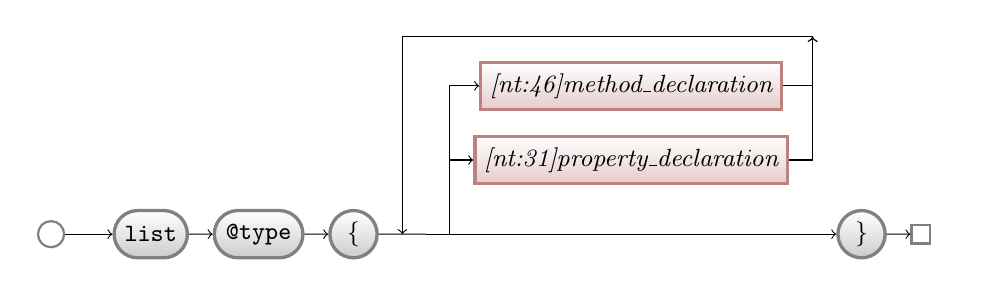
\begin{tikzpicture}
  \matrix[column sep=\ruleMatrixColumnSeparation, row sep=\ruleMatrixRowSeparation] {
    & & & & & & & & & \node (p3-9) [point] {}; & \\
    & & & & & & & & \node (p2-8) [nonterminal] {\nonTerminalSymbol{method\_declaration}{46}}; & \\
    & & & & & & & & \node (p1-8) [nonterminal] {\nonTerminalSymbol{property\_declaration}{31}}; & \\
    \node (P0start) [firstPoint] {}; & & \node (p0-2) [terminal] {list}; & \node (p0-3) [terminal] {@type}; & \node (p0-4) [terminal] {\{}; & \node (p0-5) [point] {}; & \node (p0-6) [point] {}; & \node (p0-7) [point] {}; & & & \node (p0-10) [terminal] {\}}; & \node (p0-11) [lastPoint] {}; & \\
  };
  \draw[->] (P0start) -- (p0-2) ;
  \draw[->] (p0-2) -- (p0-3) ;
  \draw[->] (p0-3) -- (p0-4) ;
  \draw (p0-4) -- (p0-6) ;
  \draw[->] (p0-7) |- (p1-8) ;
  \draw[->] (p0-7) |- (p2-8) ;
  \draw[->] (p3-9) -| (p0-5) ;
  \draw[->] (p1-8) -| (p3-9) ;
  \draw[->] (p2-8) -| (p3-9) ;
  \draw[->] (p0-6) -- (p0-10) ;
  \draw[->] (p0-10) -- (p0-11) ;
\end{tikzpicture}

\ruleSubsection{galgas4DeclarationsSyntax}{type-listmap}{41}

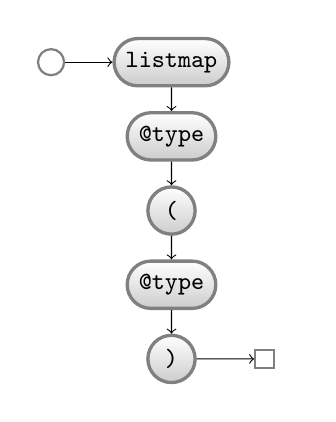
\begin{tikzpicture}
  \matrix[column sep=\ruleMatrixColumnSeparation, row sep=\ruleMatrixRowSeparation] {
    \node (P0start) [firstPoint] {}; & & \node (p4-2) [terminal] {listmap}; & \\
    & & \node (p3-2) [terminal] {@type}; & \\
    & & \node (p2-2) [terminal] {(}; & \\
    & & \node (p1-2) [terminal] {@type}; & \\
    & & \node (p0-2) [terminal] {)}; & \node (p0-3) [lastPoint] {}; & \\
  };
  \draw[->] (P0start) -- (p4-2) ;
  \draw[->] (p4-2) -- (p3-2) ;
  \draw[->] (p3-2) -- (p2-2) ;
  \draw[->] (p2-2) -- (p1-2) ;
  \draw[->] (p1-2) -- (p0-2) ;
  \draw[->] (p0-2) -- (p0-3) ;
\end{tikzpicture}

\ruleSubsection{galgas4DeclarationsSyntax}{type-dict}{69}

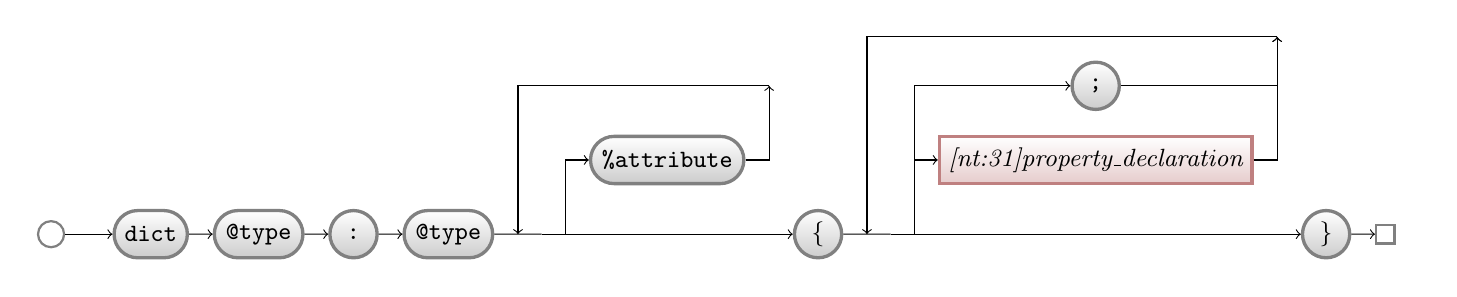
\begin{tikzpicture}
  \matrix[column sep=\ruleMatrixColumnSeparation, row sep=\ruleMatrixRowSeparation] {
    & & & & & & & & & & & & & & & & \node (p3-16) [point] {}; & \\
    & & & & & & & & & & \node (p2-10) [point] {}; & & & & & \node (p2-15) [terminal] {;}; & \\
    & & & & & & & & & \node (p1-9) [terminal] {\verb=%=attribute}; & & & & & & \node (p1-15) [nonterminal] {\nonTerminalSymbol{property\_declaration}{31}}; & \\
    \node (P0start) [firstPoint] {}; & & \node (p0-2) [terminal] {dict}; & \node (p0-3) [terminal] {@type}; & \node (p0-4) [terminal] {:}; & \node (p0-5) [terminal] {@type}; & \node (p0-6) [point] {}; & \node (p0-7) [point] {}; & \node (p0-8) [point] {}; & & & \node (p0-11) [terminal] {\{}; & \node (p0-12) [point] {}; & \node (p0-13) [point] {}; & \node (p0-14) [point] {}; & & & \node (p0-17) [terminal] {\}}; & \node (p0-18) [lastPoint] {}; & \\
  };
  \draw[->] (P0start) -- (p0-2) ;
  \draw[->] (p0-2) -- (p0-3) ;
  \draw[->] (p0-3) -- (p0-4) ;
  \draw[->] (p0-4) -- (p0-5) ;
  \draw (p0-5) -- (p0-7) ;
  \draw[->] (p0-8) |- (p1-9) ;
  \draw[->] (p2-10) -| (p0-6) ;
  \draw[->] (p1-9) -| (p2-10) ;
  \draw[->] (p0-7) -- (p0-11) ;
  \draw (p0-11) -- (p0-13) ;
  \draw[->] (p0-14) |- (p1-15) ;
  \draw[->] (p0-14) |- (p2-15) ;
  \draw[->] (p3-16) -| (p0-12) ;
  \draw[->] (p1-15) -| (p3-16) ;
  \draw[->] (p2-15) -| (p3-16) ;
  \draw[->] (p0-13) -- (p0-17) ;
  \draw[->] (p0-17) -- (p0-18) ;
\end{tikzpicture}

\ruleSubsection{galgas4DeclarationsSyntax}{type-map}{184}

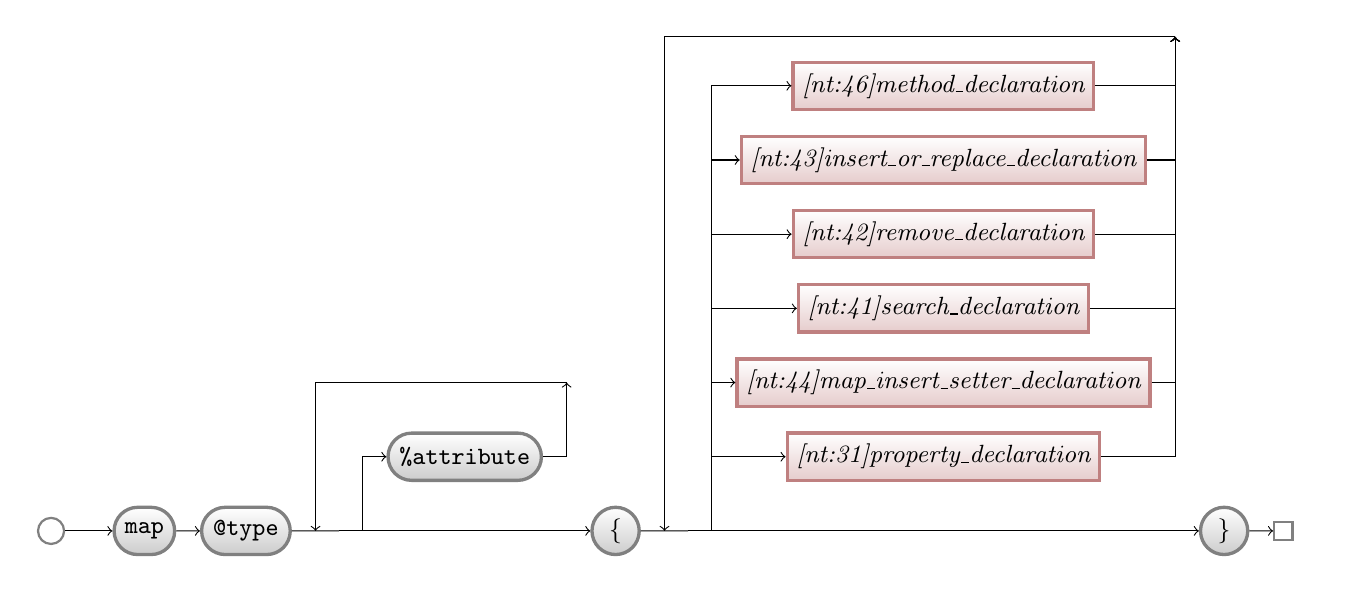
\begin{tikzpicture}
  \matrix[column sep=\ruleMatrixColumnSeparation, row sep=\ruleMatrixRowSeparation] {
    & & & & & & & & & & & & & & \node (p7-14) [point] {}; & \\
    & & & & & & & & & & & & & \node (p6-13) [nonterminal] {\nonTerminalSymbol{method\_declaration}{46}}; & \\
    & & & & & & & & & & & & & \node (p5-13) [nonterminal] {\nonTerminalSymbol{insert\_or\_replace\_declaration}{43}}; & \\
    & & & & & & & & & & & & & \node (p4-13) [nonterminal] {\nonTerminalSymbol{remove\_declaration}{42}}; & \\
    & & & & & & & & & & & & & \node (p3-13) [nonterminal] {\nonTerminalSymbol{search\_declaration}{41}}; & \\
    & & & & & & & & \node (p2-8) [point] {}; & & & & & \node (p2-13) [nonterminal] {\nonTerminalSymbol{map\_insert\_setter\_declaration}{44}}; & \\
    & & & & & & & \node (p1-7) [terminal] {\verb=%=attribute}; & & & & & & \node (p1-13) [nonterminal] {\nonTerminalSymbol{property\_declaration}{31}}; & \\
    \node (P0start) [firstPoint] {}; & & \node (p0-2) [terminal] {map}; & \node (p0-3) [terminal] {@type}; & \node (p0-4) [point] {}; & \node (p0-5) [point] {}; & \node (p0-6) [point] {}; & & & \node (p0-9) [terminal] {\{}; & \node (p0-10) [point] {}; & \node (p0-11) [point] {}; & \node (p0-12) [point] {}; & & & \node (p0-15) [terminal] {\}}; & \node (p0-16) [lastPoint] {}; & \\
  };
  \draw[->] (P0start) -- (p0-2) ;
  \draw[->] (p0-2) -- (p0-3) ;
  \draw (p0-3) -- (p0-5) ;
  \draw[->] (p0-6) |- (p1-7) ;
  \draw[->] (p2-8) -| (p0-4) ;
  \draw[->] (p1-7) -| (p2-8) ;
  \draw[->] (p0-5) -- (p0-9) ;
  \draw (p0-9) -- (p0-11) ;
  \draw[->] (p0-12) |- (p1-13) ;
  \draw[->] (p0-12) |- (p2-13) ;
  \draw[->] (p0-12) |- (p3-13) ;
  \draw[->] (p0-12) |- (p4-13) ;
  \draw[->] (p0-12) |- (p5-13) ;
  \draw[->] (p0-12) |- (p6-13) ;
  \draw[->] (p7-14) -| (p0-10) ;
  \draw[->] (p1-13) -| (p7-14) ;
  \draw[->] (p2-13) -| (p7-14) ;
  \draw[->] (p3-13) -| (p7-14) ;
  \draw[->] (p4-13) -| (p7-14) ;
  \draw[->] (p5-13) -| (p7-14) ;
  \draw[->] (p6-13) -| (p7-14) ;
  \draw[->] (p0-11) -- (p0-15) ;
  \draw[->] (p0-15) -- (p0-16) ;
\end{tikzpicture}

\ruleSubsection{galgas4DeclarationsSyntax}{type-sorted-list}{81}

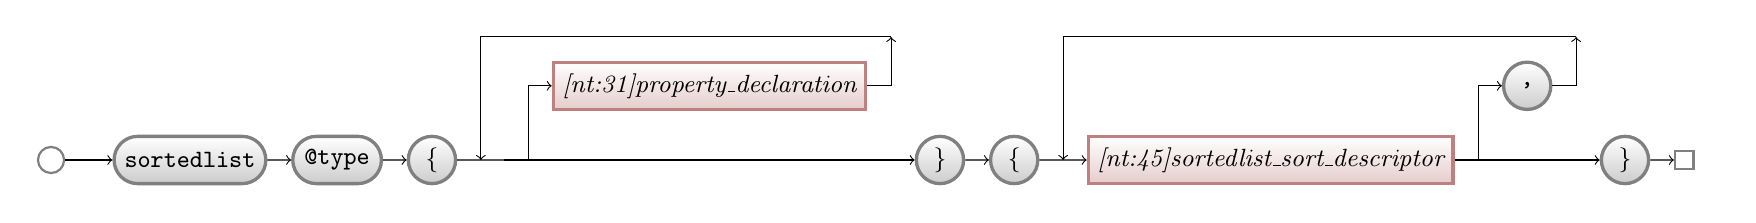
\begin{tikzpicture}
  \matrix[column sep=\ruleMatrixColumnSeparation, row sep=\ruleMatrixRowSeparation] {
    & & & & & & & & & \node (p2-9) [point] {}; & & & & & & & \node (p2-16) [point] {}; & \\
    & & & & & & & & \node (p1-8) [nonterminal] {\nonTerminalSymbol{property\_declaration}{31}}; & & & & & & & \node (p1-15) [terminal] {,}; & \\
    \node (P0start) [firstPoint] {}; & & \node (p0-2) [terminal] {sortedlist}; & \node (p0-3) [terminal] {@type}; & \node (p0-4) [terminal] {\{}; & \node (p0-5) [point] {}; & \node (p0-6) [point] {}; & \node (p0-7) [point] {}; & & & \node (p0-10) [terminal] {\}}; & \node (p0-11) [terminal] {\{}; & \node (p0-12) [point] {}; & \node (p0-13) [nonterminal] {\nonTerminalSymbol{sortedlist\_sort\_descriptor}{45}}; & \node (p0-14) [point] {}; & & & \node (p0-17) [terminal] {\}}; & \node (p0-18) [lastPoint] {}; & \\
  };
  \draw[->] (P0start) -- (p0-2) ;
  \draw[->] (p0-2) -- (p0-3) ;
  \draw[->] (p0-3) -- (p0-4) ;
  \draw (p0-4) -- (p0-6) ;
  \draw[->] (p0-7) |- (p1-8) ;
  \draw[->] (p2-9) -| (p0-5) ;
  \draw[->] (p1-8) -| (p2-9) ;
  \draw[->] (p0-6) -- (p0-10) ;
  \draw[->] (p0-10) -- (p0-11) ;
  \draw[->] (p0-11) -- (p0-13) ;
  \draw[->] (p0-14) |- (p1-15) ;
  \draw[->] (p2-16) -| (p0-12) ;
  \draw[->] (p1-15) -| (p2-16) ;
  \draw[->] (p0-13) -- (p0-17) ;
  \draw[->] (p0-17) -- (p0-18) ;
\end{tikzpicture}

\ruleSubsection{galgas4DeclarationsSyntax}{type-struct}{49}

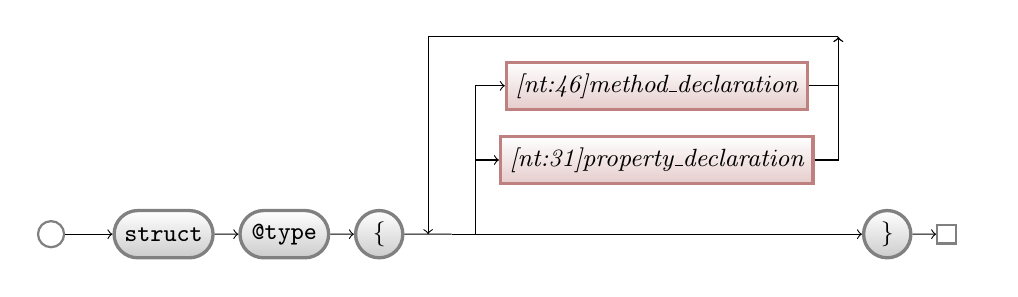
\begin{tikzpicture}
  \matrix[column sep=\ruleMatrixColumnSeparation, row sep=\ruleMatrixRowSeparation] {
    & & & & & & & & & \node (p3-9) [point] {}; & \\
    & & & & & & & & \node (p2-8) [nonterminal] {\nonTerminalSymbol{method\_declaration}{46}}; & \\
    & & & & & & & & \node (p1-8) [nonterminal] {\nonTerminalSymbol{property\_declaration}{31}}; & \\
    \node (P0start) [firstPoint] {}; & & \node (p0-2) [terminal] {struct}; & \node (p0-3) [terminal] {@type}; & \node (p0-4) [terminal] {\{}; & \node (p0-5) [point] {}; & \node (p0-6) [point] {}; & \node (p0-7) [point] {}; & & & \node (p0-10) [terminal] {\}}; & \node (p0-11) [lastPoint] {}; & \\
  };
  \draw[->] (P0start) -- (p0-2) ;
  \draw[->] (p0-2) -- (p0-3) ;
  \draw[->] (p0-3) -- (p0-4) ;
  \draw (p0-4) -- (p0-6) ;
  \draw[->] (p0-7) |- (p1-8) ;
  \draw[->] (p0-7) |- (p2-8) ;
  \draw[->] (p3-9) -| (p0-5) ;
  \draw[->] (p1-8) -| (p3-9) ;
  \draw[->] (p2-8) -| (p3-9) ;
  \draw[->] (p0-6) -- (p0-10) ;
  \draw[->] (p0-10) -- (p0-11) ;
\end{tikzpicture}

\ruleSubsection{galgas4DeclarationsSyntax}{extension-abstract-getter}{52}

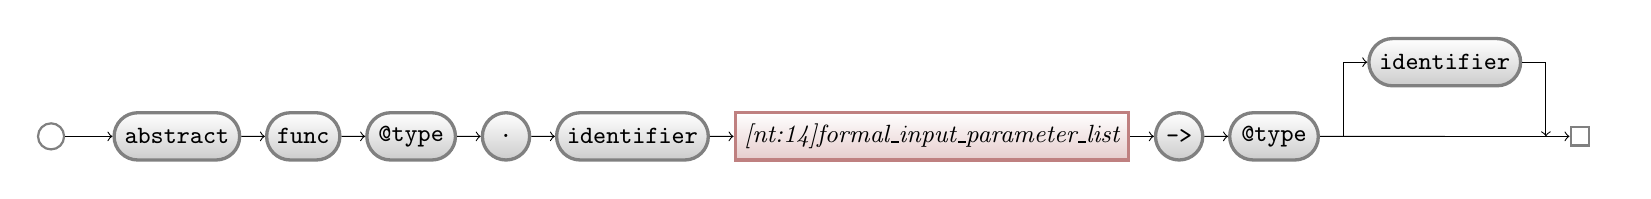
\begin{tikzpicture}
  \matrix[column sep=\ruleMatrixColumnSeparation, row sep=\ruleMatrixRowSeparation] {
    & & & & & & & & & & & \node (p1-11) [terminal] {identifier}; & \\
    \node (P0start) [firstPoint] {}; & & \node (p0-2) [terminal] {abstract}; & \node (p0-3) [terminal] {func}; & \node (p0-4) [terminal] {@type}; & \node (p0-5) [terminal] {.}; & \node (p0-6) [terminal] {identifier}; & \node (p0-7) [nonterminal] {\nonTerminalSymbol{formal\_input\_parameter\_list}{14}}; & \node (p0-8) [terminal] {->}; & \node (p0-9) [terminal] {@type}; & \node (p0-10) [point] {}; & \node (p0-11) [point] {}; & \node (p0-12) [point] {}; & \node (p0-13) [lastPoint] {}; & \\
  };
  \draw[->] (P0start) -- (p0-2) ;
  \draw[->] (p0-2) -- (p0-3) ;
  \draw[->] (p0-3) -- (p0-4) ;
  \draw[->] (p0-4) -- (p0-5) ;
  \draw[->] (p0-5) -- (p0-6) ;
  \draw[->] (p0-6) -- (p0-7) ;
  \draw[->] (p0-7) -- (p0-8) ;
  \draw[->] (p0-8) -- (p0-9) ;
  \draw (p0-9) -- (p0-11) ;
  \draw[->] (p0-10) |- (p1-11) ;
  \draw (p0-11) -- (p0-12) ;
  \draw[->] (p1-11) -| (p0-12) ;
  \draw[->] (p0-12) -- (p0-13) ;
\end{tikzpicture}

\ruleSubsection{galgas4DeclarationsSyntax}{extension-abstract-method}{43}

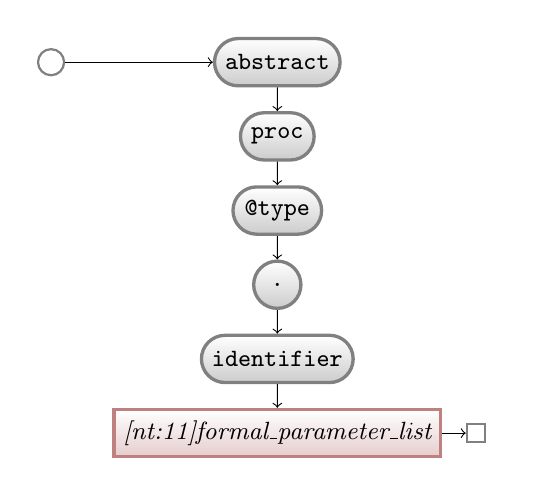
\begin{tikzpicture}
  \matrix[column sep=\ruleMatrixColumnSeparation, row sep=\ruleMatrixRowSeparation] {
    \node (P0start) [firstPoint] {}; & & \node (p5-2) [terminal] {abstract}; & \\
    & & \node (p4-2) [terminal] {proc}; & \\
    & & \node (p3-2) [terminal] {@type}; & \\
    & & \node (p2-2) [terminal] {.}; & \\
    & & \node (p1-2) [terminal] {identifier}; & \\
    & & \node (p0-2) [nonterminal] {\nonTerminalSymbol{formal\_parameter\_list}{11}}; & \node (p0-3) [lastPoint] {}; & \\
  };
  \draw[->] (P0start) -- (p5-2) ;
  \draw[->] (p5-2) -- (p4-2) ;
  \draw[->] (p4-2) -- (p3-2) ;
  \draw[->] (p3-2) -- (p2-2) ;
  \draw[->] (p2-2) -- (p1-2) ;
  \draw[->] (p1-2) -- (p0-2) ;
  \draw[->] (p0-2) -- (p0-3) ;
\end{tikzpicture}

\ruleSubsection{galgas4DeclarationsSyntax}{extension-getter}{64}

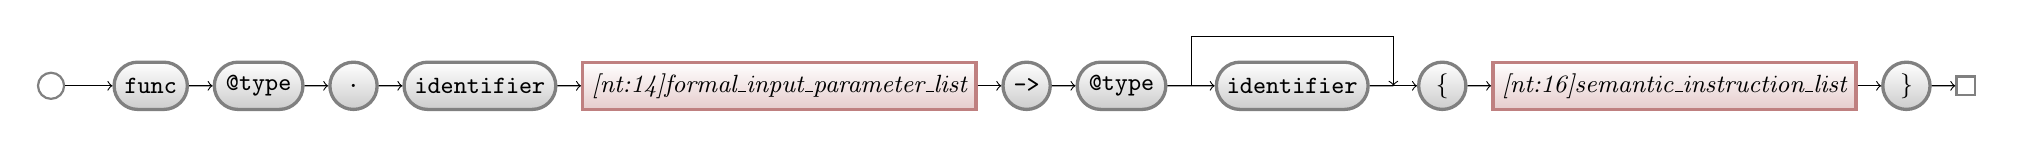
\begin{tikzpicture}
  \matrix[column sep=\ruleMatrixColumnSeparation, row sep=\ruleMatrixRowSeparation] {
    & & & & & & & & & & \node (p1-10) [point] {}; & \\
    \node (P0start) [firstPoint] {}; & & \node (p0-2) [terminal] {func}; & \node (p0-3) [terminal] {@type}; & \node (p0-4) [terminal] {.}; & \node (p0-5) [terminal] {identifier}; & \node (p0-6) [nonterminal] {\nonTerminalSymbol{formal\_input\_parameter\_list}{14}}; & \node (p0-7) [terminal] {->}; & \node (p0-8) [terminal] {@type}; & \node (p0-9) [point] {}; & \node (p0-10) [terminal] {identifier}; & \node (p0-11) [point] {}; & \node (p0-12) [terminal] {\{}; & \node (p0-13) [nonterminal] {\nonTerminalSymbol{semantic\_instruction\_list}{16}}; & \node (p0-14) [terminal] {\}}; & \node (p0-15) [lastPoint] {}; & \\
  };
  \draw[->] (P0start) -- (p0-2) ;
  \draw[->] (p0-2) -- (p0-3) ;
  \draw[->] (p0-3) -- (p0-4) ;
  \draw[->] (p0-4) -- (p0-5) ;
  \draw[->] (p0-5) -- (p0-6) ;
  \draw[->] (p0-6) -- (p0-7) ;
  \draw[->] (p0-7) -- (p0-8) ;
  \draw[->] (p0-8) -- (p0-10) ;
  \draw (p0-9) |- (p1-10) ;
  \draw (p0-10) -- (p0-11) ;
  \draw[->] (p1-10) -| (p0-11) ;
  \draw[->] (p0-11) -- (p0-12) ;
  \draw[->] (p0-12) -- (p0-13) ;
  \draw[->] (p0-13) -- (p0-14) ;
  \draw[->] (p0-14) -- (p0-15) ;
\end{tikzpicture}

\ruleSubsection{galgas4DeclarationsSyntax}{extension-method}{53}

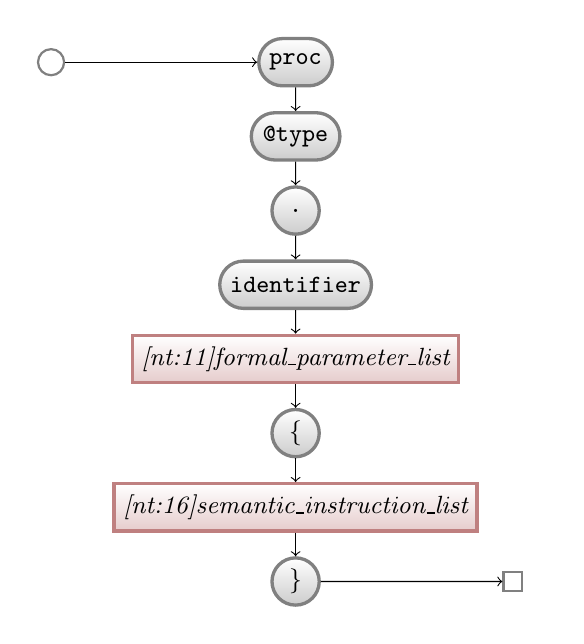
\begin{tikzpicture}
  \matrix[column sep=\ruleMatrixColumnSeparation, row sep=\ruleMatrixRowSeparation] {
    \node (P0start) [firstPoint] {}; & & \node (p7-2) [terminal] {proc}; & \\
    & & \node (p6-2) [terminal] {@type}; & \\
    & & \node (p5-2) [terminal] {.}; & \\
    & & \node (p4-2) [terminal] {identifier}; & \\
    & & \node (p3-2) [nonterminal] {\nonTerminalSymbol{formal\_parameter\_list}{11}}; & \\
    & & \node (p2-2) [terminal] {\{}; & \\
    & & \node (p1-2) [nonterminal] {\nonTerminalSymbol{semantic\_instruction\_list}{16}}; & \\
    & & \node (p0-2) [terminal] {\}}; & \node (p0-3) [lastPoint] {}; & \\
  };
  \draw[->] (P0start) -- (p7-2) ;
  \draw[->] (p7-2) -- (p6-2) ;
  \draw[->] (p6-2) -- (p5-2) ;
  \draw[->] (p5-2) -- (p4-2) ;
  \draw[->] (p4-2) -- (p3-2) ;
  \draw[->] (p3-2) -- (p2-2) ;
  \draw[->] (p2-2) -- (p1-2) ;
  \draw[->] (p1-2) -- (p0-2) ;
  \draw[->] (p0-2) -- (p0-3) ;
\end{tikzpicture}

\ruleSubsection{galgas4DeclarationsSyntax}{extension-setter}{52}

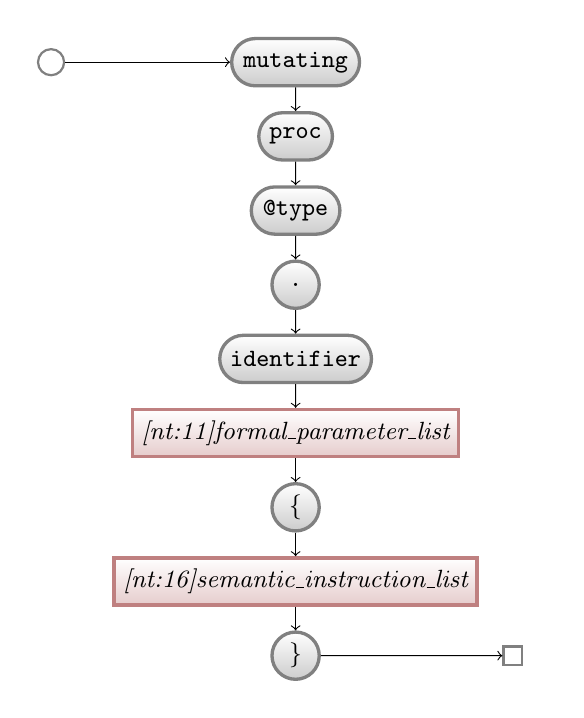
\begin{tikzpicture}
  \matrix[column sep=\ruleMatrixColumnSeparation, row sep=\ruleMatrixRowSeparation] {
    \node (P0start) [firstPoint] {}; & & \node (p8-2) [terminal] {mutating}; & \\
    & & \node (p7-2) [terminal] {proc}; & \\
    & & \node (p6-2) [terminal] {@type}; & \\
    & & \node (p5-2) [terminal] {.}; & \\
    & & \node (p4-2) [terminal] {identifier}; & \\
    & & \node (p3-2) [nonterminal] {\nonTerminalSymbol{formal\_parameter\_list}{11}}; & \\
    & & \node (p2-2) [terminal] {\{}; & \\
    & & \node (p1-2) [nonterminal] {\nonTerminalSymbol{semantic\_instruction\_list}{16}}; & \\
    & & \node (p0-2) [terminal] {\}}; & \node (p0-3) [lastPoint] {}; & \\
  };
  \draw[->] (P0start) -- (p8-2) ;
  \draw[->] (p8-2) -- (p7-2) ;
  \draw[->] (p7-2) -- (p6-2) ;
  \draw[->] (p6-2) -- (p5-2) ;
  \draw[->] (p5-2) -- (p4-2) ;
  \draw[->] (p4-2) -- (p3-2) ;
  \draw[->] (p3-2) -- (p2-2) ;
  \draw[->] (p2-2) -- (p1-2) ;
  \draw[->] (p1-2) -- (p0-2) ;
  \draw[->] (p0-2) -- (p0-3) ;
\end{tikzpicture}

\ruleSubsection{galgas4DeclarationsSyntax}{extension-overriding-abstract-getter}{53}

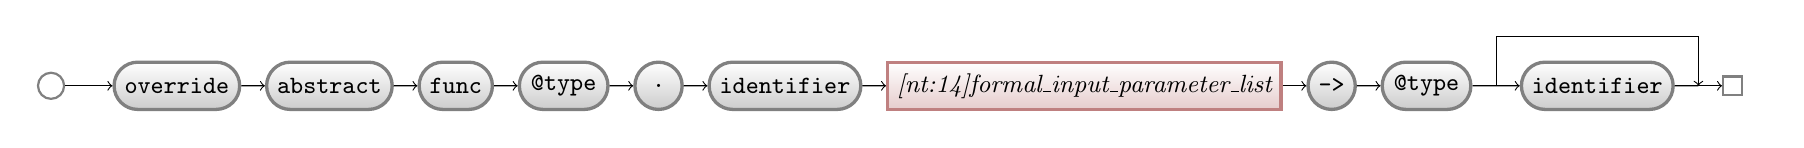
\begin{tikzpicture}
  \matrix[column sep=\ruleMatrixColumnSeparation, row sep=\ruleMatrixRowSeparation] {
    & & & & & & & & & & & & \node (p1-12) [point] {}; & \\
    \node (P0start) [firstPoint] {}; & & \node (p0-2) [terminal] {override}; & \node (p0-3) [terminal] {abstract}; & \node (p0-4) [terminal] {func}; & \node (p0-5) [terminal] {@type}; & \node (p0-6) [terminal] {.}; & \node (p0-7) [terminal] {identifier}; & \node (p0-8) [nonterminal] {\nonTerminalSymbol{formal\_input\_parameter\_list}{14}}; & \node (p0-9) [terminal] {->}; & \node (p0-10) [terminal] {@type}; & \node (p0-11) [point] {}; & \node (p0-12) [terminal] {identifier}; & \node (p0-13) [point] {}; & \node (p0-14) [lastPoint] {}; & \\
  };
  \draw[->] (P0start) -- (p0-2) ;
  \draw[->] (p0-2) -- (p0-3) ;
  \draw[->] (p0-3) -- (p0-4) ;
  \draw[->] (p0-4) -- (p0-5) ;
  \draw[->] (p0-5) -- (p0-6) ;
  \draw[->] (p0-6) -- (p0-7) ;
  \draw[->] (p0-7) -- (p0-8) ;
  \draw[->] (p0-8) -- (p0-9) ;
  \draw[->] (p0-9) -- (p0-10) ;
  \draw[->] (p0-10) -- (p0-12) ;
  \draw (p0-11) |- (p1-12) ;
  \draw (p0-12) -- (p0-13) ;
  \draw[->] (p1-12) -| (p0-13) ;
  \draw[->] (p0-13) -- (p0-14) ;
\end{tikzpicture}

\ruleSubsection{galgas4DeclarationsSyntax}{extension-overriding-abstract-method}{44}

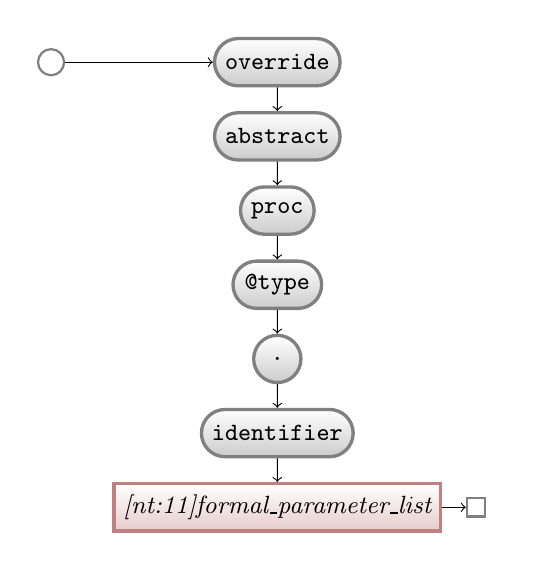
\begin{tikzpicture}
  \matrix[column sep=\ruleMatrixColumnSeparation, row sep=\ruleMatrixRowSeparation] {
    \node (P0start) [firstPoint] {}; & & \node (p6-2) [terminal] {override}; & \\
    & & \node (p5-2) [terminal] {abstract}; & \\
    & & \node (p4-2) [terminal] {proc}; & \\
    & & \node (p3-2) [terminal] {@type}; & \\
    & & \node (p2-2) [terminal] {.}; & \\
    & & \node (p1-2) [terminal] {identifier}; & \\
    & & \node (p0-2) [nonterminal] {\nonTerminalSymbol{formal\_parameter\_list}{11}}; & \node (p0-3) [lastPoint] {}; & \\
  };
  \draw[->] (P0start) -- (p6-2) ;
  \draw[->] (p6-2) -- (p5-2) ;
  \draw[->] (p5-2) -- (p4-2) ;
  \draw[->] (p4-2) -- (p3-2) ;
  \draw[->] (p3-2) -- (p2-2) ;
  \draw[->] (p2-2) -- (p1-2) ;
  \draw[->] (p1-2) -- (p0-2) ;
  \draw[->] (p0-2) -- (p0-3) ;
\end{tikzpicture}

\ruleSubsection{galgas4DeclarationsSyntax}{extension-overriding-getter}{65}

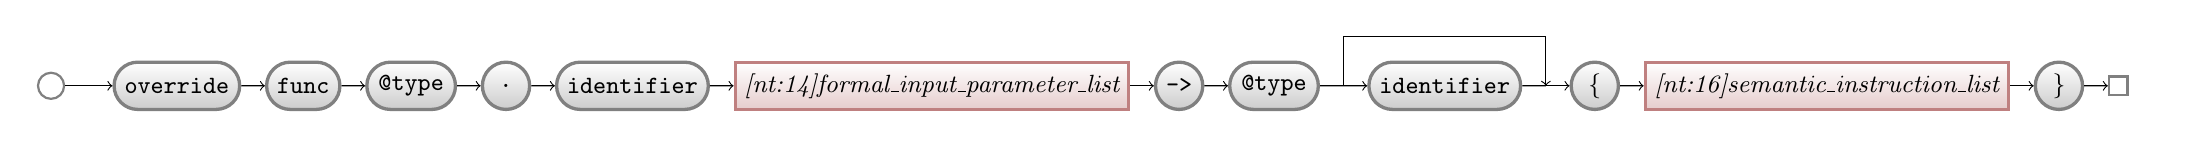
\begin{tikzpicture}
  \matrix[column sep=\ruleMatrixColumnSeparation, row sep=\ruleMatrixRowSeparation] {
    & & & & & & & & & & & \node (p1-11) [point] {}; & \\
    \node (P0start) [firstPoint] {}; & & \node (p0-2) [terminal] {override}; & \node (p0-3) [terminal] {func}; & \node (p0-4) [terminal] {@type}; & \node (p0-5) [terminal] {.}; & \node (p0-6) [terminal] {identifier}; & \node (p0-7) [nonterminal] {\nonTerminalSymbol{formal\_input\_parameter\_list}{14}}; & \node (p0-8) [terminal] {->}; & \node (p0-9) [terminal] {@type}; & \node (p0-10) [point] {}; & \node (p0-11) [terminal] {identifier}; & \node (p0-12) [point] {}; & \node (p0-13) [terminal] {\{}; & \node (p0-14) [nonterminal] {\nonTerminalSymbol{semantic\_instruction\_list}{16}}; & \node (p0-15) [terminal] {\}}; & \node (p0-16) [lastPoint] {}; & \\
  };
  \draw[->] (P0start) -- (p0-2) ;
  \draw[->] (p0-2) -- (p0-3) ;
  \draw[->] (p0-3) -- (p0-4) ;
  \draw[->] (p0-4) -- (p0-5) ;
  \draw[->] (p0-5) -- (p0-6) ;
  \draw[->] (p0-6) -- (p0-7) ;
  \draw[->] (p0-7) -- (p0-8) ;
  \draw[->] (p0-8) -- (p0-9) ;
  \draw[->] (p0-9) -- (p0-11) ;
  \draw (p0-10) |- (p1-11) ;
  \draw (p0-11) -- (p0-12) ;
  \draw[->] (p1-11) -| (p0-12) ;
  \draw[->] (p0-12) -- (p0-13) ;
  \draw[->] (p0-13) -- (p0-14) ;
  \draw[->] (p0-14) -- (p0-15) ;
  \draw[->] (p0-15) -- (p0-16) ;
\end{tikzpicture}

\ruleSubsection{galgas4DeclarationsSyntax}{extension-overriding-method}{53}

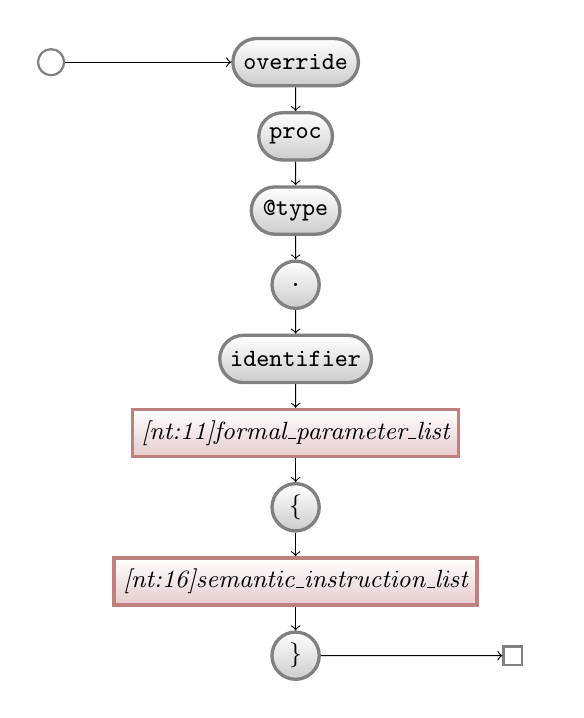
\begin{tikzpicture}
  \matrix[column sep=\ruleMatrixColumnSeparation, row sep=\ruleMatrixRowSeparation] {
    \node (P0start) [firstPoint] {}; & & \node (p8-2) [terminal] {override}; & \\
    & & \node (p7-2) [terminal] {proc}; & \\
    & & \node (p6-2) [terminal] {@type}; & \\
    & & \node (p5-2) [terminal] {.}; & \\
    & & \node (p4-2) [terminal] {identifier}; & \\
    & & \node (p3-2) [nonterminal] {\nonTerminalSymbol{formal\_parameter\_list}{11}}; & \\
    & & \node (p2-2) [terminal] {\{}; & \\
    & & \node (p1-2) [nonterminal] {\nonTerminalSymbol{semantic\_instruction\_list}{16}}; & \\
    & & \node (p0-2) [terminal] {\}}; & \node (p0-3) [lastPoint] {}; & \\
  };
  \draw[->] (P0start) -- (p8-2) ;
  \draw[->] (p8-2) -- (p7-2) ;
  \draw[->] (p7-2) -- (p6-2) ;
  \draw[->] (p6-2) -- (p5-2) ;
  \draw[->] (p5-2) -- (p4-2) ;
  \draw[->] (p4-2) -- (p3-2) ;
  \draw[->] (p3-2) -- (p2-2) ;
  \draw[->] (p2-2) -- (p1-2) ;
  \draw[->] (p1-2) -- (p0-2) ;
  \draw[->] (p0-2) -- (p0-3) ;
\end{tikzpicture}

\ruleSubsection{galgas4LexiqueComponentSyntax}{lexique-component}{452}

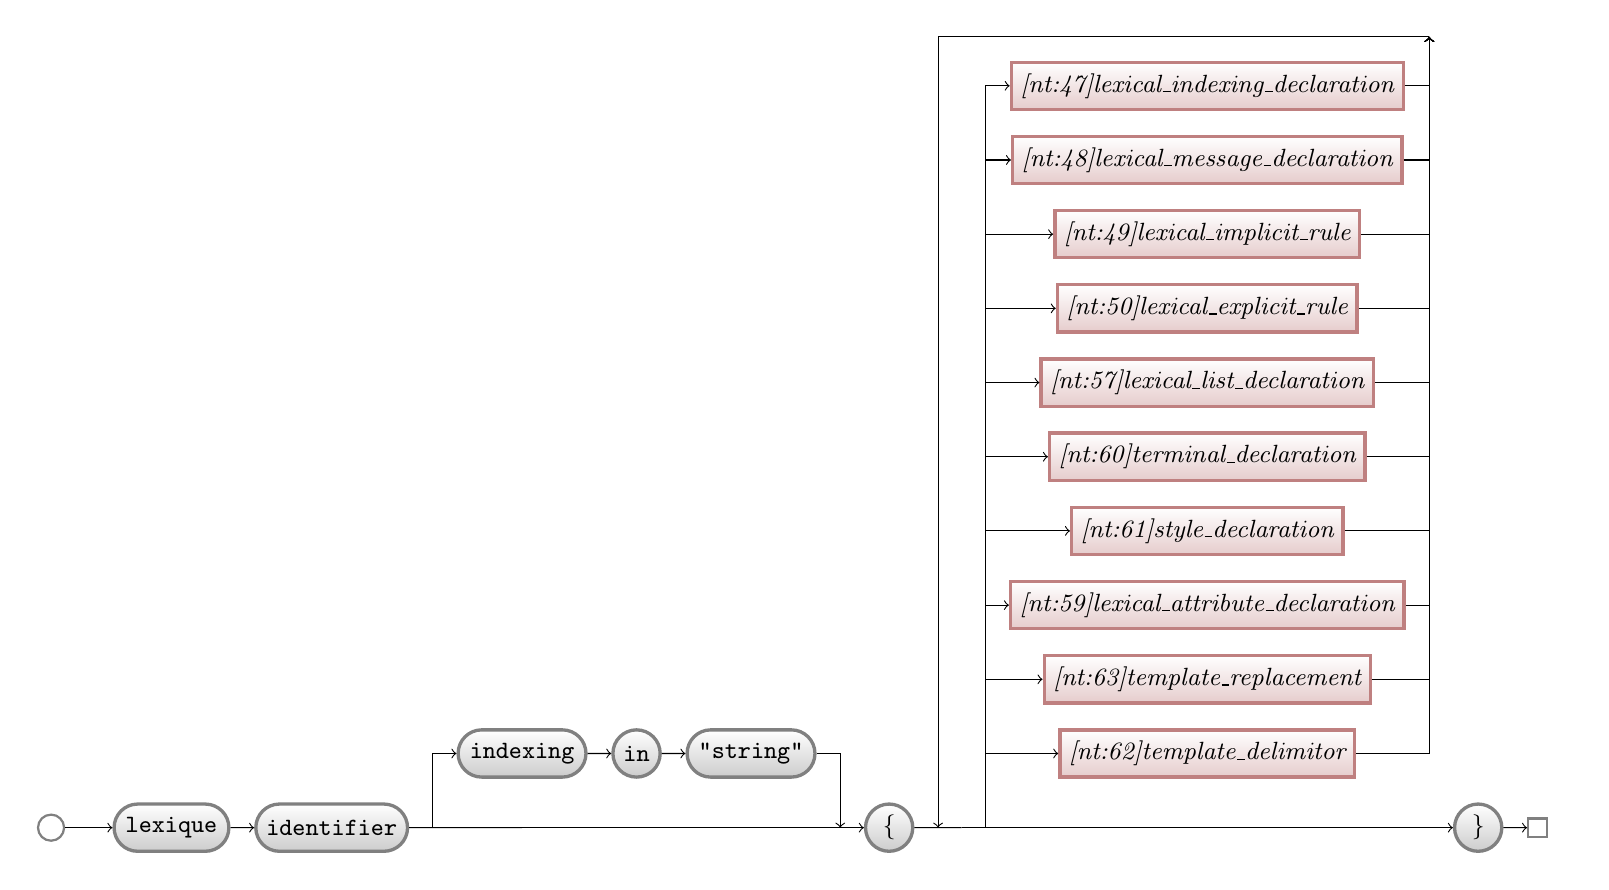
\begin{tikzpicture}
  \matrix[column sep=\ruleMatrixColumnSeparation, row sep=\ruleMatrixRowSeparation] {
    & & & & & & & & & & & & & & \node (p11-14) [point] {}; & \\
    & & & & & & & & & & & & & \node (p10-13) [nonterminal] {\nonTerminalSymbol{lexical\_indexing\_declaration}{47}}; & \\
    & & & & & & & & & & & & & \node (p9-13) [nonterminal] {\nonTerminalSymbol{lexical\_message\_declaration}{48}}; & \\
    & & & & & & & & & & & & & \node (p8-13) [nonterminal] {\nonTerminalSymbol{lexical\_implicit\_rule}{49}}; & \\
    & & & & & & & & & & & & & \node (p7-13) [nonterminal] {\nonTerminalSymbol{lexical\_explicit\_rule}{50}}; & \\
    & & & & & & & & & & & & & \node (p6-13) [nonterminal] {\nonTerminalSymbol{lexical\_list\_declaration}{57}}; & \\
    & & & & & & & & & & & & & \node (p5-13) [nonterminal] {\nonTerminalSymbol{terminal\_declaration}{60}}; & \\
    & & & & & & & & & & & & & \node (p4-13) [nonterminal] {\nonTerminalSymbol{style\_declaration}{61}}; & \\
    & & & & & & & & & & & & & \node (p3-13) [nonterminal] {\nonTerminalSymbol{lexical\_attribute\_declaration}{59}}; & \\
    & & & & & & & & & & & & & \node (p2-13) [nonterminal] {\nonTerminalSymbol{template\_replacement}{63}}; & \\
    & & & & & \node (p1-5) [terminal] {indexing}; & \node (p1-6) [terminal] {in}; & \node (p1-7) [terminal] {"string"}; & & & & & & \node (p1-13) [nonterminal] {\nonTerminalSymbol{template\_delimitor}{62}}; & \\
    \node (P0start) [firstPoint] {}; & & \node (p0-2) [terminal] {lexique}; & \node (p0-3) [terminal] {identifier}; & \node (p0-4) [point] {}; & \node (p0-5) [point] {}; & & & \node (p0-8) [point] {}; & \node (p0-9) [terminal] {\{}; & \node (p0-10) [point] {}; & \node (p0-11) [point] {}; & \node (p0-12) [point] {}; & & & \node (p0-15) [terminal] {\}}; & \node (p0-16) [lastPoint] {}; & \\
  };
  \draw[->] (P0start) -- (p0-2) ;
  \draw[->] (p0-2) -- (p0-3) ;
  \draw (p0-3) -- (p0-5) ;
  \draw[->] (p0-4) |- (p1-5) ;
  \draw[->] (p1-5) -- (p1-6) ;
  \draw[->] (p1-6) -- (p1-7) ;
  \draw (p0-5) -- (p0-8) ;
  \draw[->] (p1-7) -| (p0-8) ;
  \draw[->] (p0-8) -- (p0-9) ;
  \draw (p0-9) -- (p0-11) ;
  \draw[->] (p0-12) |- (p1-13) ;
  \draw[->] (p0-12) |- (p2-13) ;
  \draw[->] (p0-12) |- (p3-13) ;
  \draw[->] (p0-12) |- (p4-13) ;
  \draw[->] (p0-12) |- (p5-13) ;
  \draw[->] (p0-12) |- (p6-13) ;
  \draw[->] (p0-12) |- (p7-13) ;
  \draw[->] (p0-12) |- (p8-13) ;
  \draw[->] (p0-12) |- (p9-13) ;
  \draw[->] (p0-12) |- (p10-13) ;
  \draw[->] (p11-14) -| (p0-10) ;
  \draw[->] (p1-13) -| (p11-14) ;
  \draw[->] (p2-13) -| (p11-14) ;
  \draw[->] (p3-13) -| (p11-14) ;
  \draw[->] (p4-13) -| (p11-14) ;
  \draw[->] (p5-13) -| (p11-14) ;
  \draw[->] (p6-13) -| (p11-14) ;
  \draw[->] (p7-13) -| (p11-14) ;
  \draw[->] (p8-13) -| (p11-14) ;
  \draw[->] (p9-13) -| (p11-14) ;
  \draw[->] (p10-13) -| (p11-14) ;
  \draw[->] (p0-11) -- (p0-15) ;
  \draw[->] (p0-15) -- (p0-16) ;
\end{tikzpicture}

\ruleSubsection{galgas4LexiqueComponentSyntax}{template-lexique-component}{102}

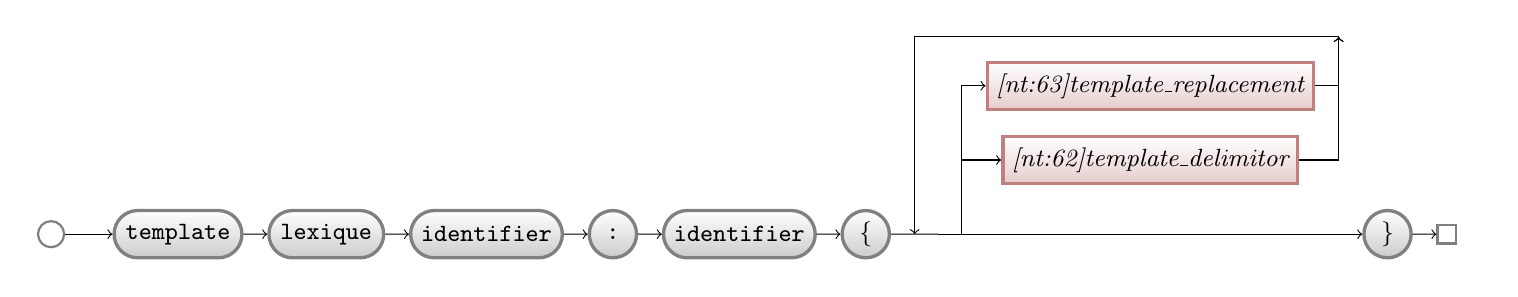
\begin{tikzpicture}
  \matrix[column sep=\ruleMatrixColumnSeparation, row sep=\ruleMatrixRowSeparation] {
    & & & & & & & & & & & & \node (p3-12) [point] {}; & \\
    & & & & & & & & & & & \node (p2-11) [nonterminal] {\nonTerminalSymbol{template\_replacement}{63}}; & \\
    & & & & & & & & & & & \node (p1-11) [nonterminal] {\nonTerminalSymbol{template\_delimitor}{62}}; & \\
    \node (P0start) [firstPoint] {}; & & \node (p0-2) [terminal] {template}; & \node (p0-3) [terminal] {lexique}; & \node (p0-4) [terminal] {identifier}; & \node (p0-5) [terminal] {:}; & \node (p0-6) [terminal] {identifier}; & \node (p0-7) [terminal] {\{}; & \node (p0-8) [point] {}; & \node (p0-9) [point] {}; & \node (p0-10) [point] {}; & & & \node (p0-13) [terminal] {\}}; & \node (p0-14) [lastPoint] {}; & \\
  };
  \draw[->] (P0start) -- (p0-2) ;
  \draw[->] (p0-2) -- (p0-3) ;
  \draw[->] (p0-3) -- (p0-4) ;
  \draw[->] (p0-4) -- (p0-5) ;
  \draw[->] (p0-5) -- (p0-6) ;
  \draw[->] (p0-6) -- (p0-7) ;
  \draw (p0-7) -- (p0-9) ;
  \draw[->] (p0-10) |- (p1-11) ;
  \draw[->] (p0-10) |- (p2-11) ;
  \draw[->] (p3-12) -| (p0-8) ;
  \draw[->] (p1-11) -| (p3-12) ;
  \draw[->] (p2-11) -| (p3-12) ;
  \draw[->] (p0-9) -- (p0-13) ;
  \draw[->] (p0-13) -- (p0-14) ;
\end{tikzpicture}

\ruleSubsection{galgas4OptionComponentSyntax}{optionCompilation}{100}

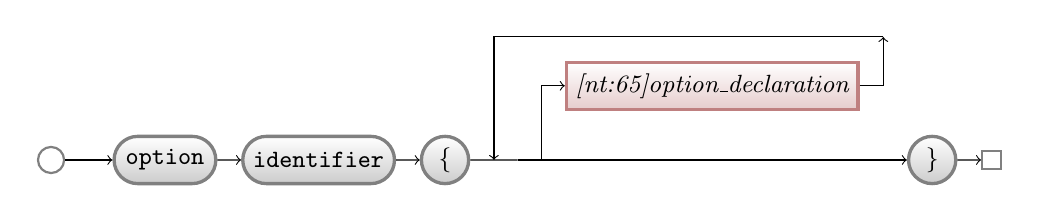
\begin{tikzpicture}
  \matrix[column sep=\ruleMatrixColumnSeparation, row sep=\ruleMatrixRowSeparation] {
    & & & & & & & & & \node (p2-9) [point] {}; & \\
    & & & & & & & & \node (p1-8) [nonterminal] {\nonTerminalSymbol{option\_declaration}{65}}; & \\
    \node (P0start) [firstPoint] {}; & & \node (p0-2) [terminal] {option}; & \node (p0-3) [terminal] {identifier}; & \node (p0-4) [terminal] {\{}; & \node (p0-5) [point] {}; & \node (p0-6) [point] {}; & \node (p0-7) [point] {}; & & & \node (p0-10) [terminal] {\}}; & \node (p0-11) [lastPoint] {}; & \\
  };
  \draw[->] (P0start) -- (p0-2) ;
  \draw[->] (p0-2) -- (p0-3) ;
  \draw[->] (p0-3) -- (p0-4) ;
  \draw (p0-4) -- (p0-6) ;
  \draw[->] (p0-7) |- (p1-8) ;
  \draw[->] (p2-9) -| (p0-5) ;
  \draw[->] (p1-8) -| (p2-9) ;
  \draw[->] (p0-6) -- (p0-10) ;
  \draw[->] (p0-10) -- (p0-11) ;
\end{tikzpicture}

\ruleSubsection{galgas4GuiComponentSyntax}{guiCompilation}{221}

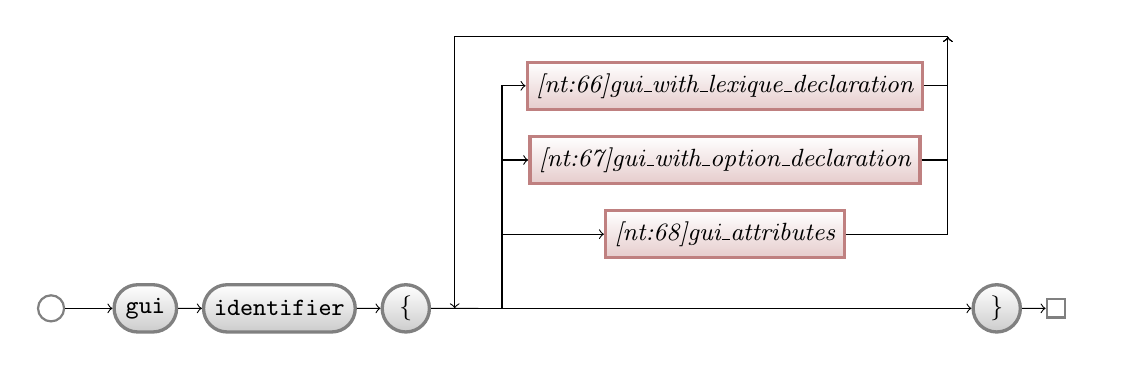
\begin{tikzpicture}
  \matrix[column sep=\ruleMatrixColumnSeparation, row sep=\ruleMatrixRowSeparation] {
    & & & & & & & & & \node (p4-9) [point] {}; & \\
    & & & & & & & & \node (p3-8) [nonterminal] {\nonTerminalSymbol{gui\_with\_lexique\_declaration}{66}}; & \\
    & & & & & & & & \node (p2-8) [nonterminal] {\nonTerminalSymbol{gui\_with\_option\_declaration}{67}}; & \\
    & & & & & & & & \node (p1-8) [nonterminal] {\nonTerminalSymbol{gui\_attributes}{68}}; & \\
    \node (P0start) [firstPoint] {}; & & \node (p0-2) [terminal] {gui}; & \node (p0-3) [terminal] {identifier}; & \node (p0-4) [terminal] {\{}; & \node (p0-5) [point] {}; & \node (p0-6) [point] {}; & \node (p0-7) [point] {}; & & & \node (p0-10) [terminal] {\}}; & \node (p0-11) [lastPoint] {}; & \\
  };
  \draw[->] (P0start) -- (p0-2) ;
  \draw[->] (p0-2) -- (p0-3) ;
  \draw[->] (p0-3) -- (p0-4) ;
  \draw (p0-4) -- (p0-6) ;
  \draw[->] (p0-7) |- (p1-8) ;
  \draw[->] (p0-7) |- (p2-8) ;
  \draw[->] (p0-7) |- (p3-8) ;
  \draw[->] (p4-9) -| (p0-5) ;
  \draw[->] (p1-8) -| (p4-9) ;
  \draw[->] (p2-8) -| (p4-9) ;
  \draw[->] (p3-8) -| (p4-9) ;
  \draw[->] (p0-6) -- (p0-10) ;
  \draw[->] (p0-10) -- (p0-11) ;
\end{tikzpicture}

\ruleSubsection{galgas4SyntaxComponentSyntax}{galgasSyntaxComponentSyntax}{214}

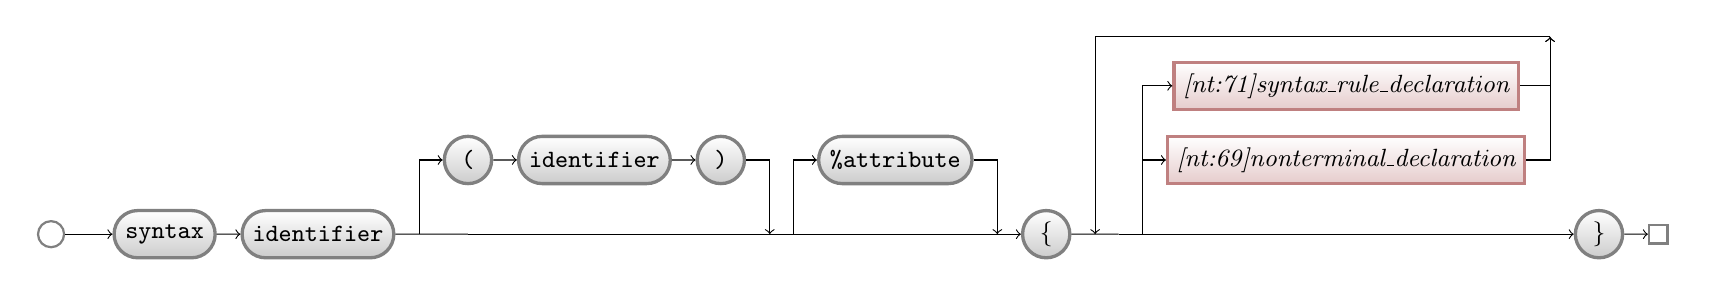
\begin{tikzpicture}
  \matrix[column sep=\ruleMatrixColumnSeparation, row sep=\ruleMatrixRowSeparation] {
    & & & & & & & & & & & & & & & & & \node (p3-17) [point] {}; & \\
    & & & & & & & & & & & & & & & & \node (p2-16) [nonterminal] {\nonTerminalSymbol{syntax\_rule\_declaration}{71}}; & \\
    & & & & & \node (p1-5) [terminal] {(}; & \node (p1-6) [terminal] {identifier}; & \node (p1-7) [terminal] {)}; & & & \node (p1-10) [terminal] {\verb=%=attribute}; & & & & & & \node (p1-16) [nonterminal] {\nonTerminalSymbol{nonterminal\_declaration}{69}}; & \\
    \node (P0start) [firstPoint] {}; & & \node (p0-2) [terminal] {syntax}; & \node (p0-3) [terminal] {identifier}; & \node (p0-4) [point] {}; & \node (p0-5) [point] {}; & & & \node (p0-8) [point] {}; & \node (p0-9) [point] {}; & \node (p0-10) [point] {}; & \node (p0-11) [point] {}; & \node (p0-12) [terminal] {\{}; & \node (p0-13) [point] {}; & \node (p0-14) [point] {}; & \node (p0-15) [point] {}; & & & \node (p0-18) [terminal] {\}}; & \node (p0-19) [lastPoint] {}; & \\
  };
  \draw[->] (P0start) -- (p0-2) ;
  \draw[->] (p0-2) -- (p0-3) ;
  \draw (p0-3) -- (p0-5) ;
  \draw[->] (p0-4) |- (p1-5) ;
  \draw[->] (p1-5) -- (p1-6) ;
  \draw[->] (p1-6) -- (p1-7) ;
  \draw (p0-5) -- (p0-8) ;
  \draw[->] (p1-7) -| (p0-8) ;
  \draw (p0-8) -- (p0-10) ;
  \draw[->] (p0-9) |- (p1-10) ;
  \draw (p0-10) -- (p0-11) ;
  \draw[->] (p1-10) -| (p0-11) ;
  \draw[->] (p0-11) -- (p0-12) ;
  \draw (p0-12) -- (p0-14) ;
  \draw[->] (p0-15) |- (p1-16) ;
  \draw[->] (p0-15) |- (p2-16) ;
  \draw[->] (p3-17) -| (p0-13) ;
  \draw[->] (p1-16) -| (p3-17) ;
  \draw[->] (p2-16) -| (p3-17) ;
  \draw[->] (p0-14) -- (p0-18) ;
  \draw[->] (p0-18) -- (p0-19) ;
\end{tikzpicture}

\ruleSubsection{galgas4SyntaxComponentSyntax}{galgasSyntaxComponentSyntax}{261}

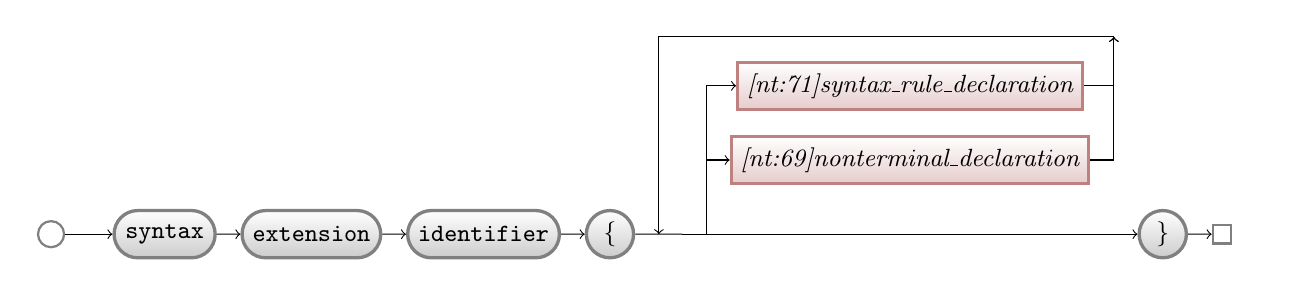
\begin{tikzpicture}
  \matrix[column sep=\ruleMatrixColumnSeparation, row sep=\ruleMatrixRowSeparation] {
    & & & & & & & & & & \node (p3-10) [point] {}; & \\
    & & & & & & & & & \node (p2-9) [nonterminal] {\nonTerminalSymbol{syntax\_rule\_declaration}{71}}; & \\
    & & & & & & & & & \node (p1-9) [nonterminal] {\nonTerminalSymbol{nonterminal\_declaration}{69}}; & \\
    \node (P0start) [firstPoint] {}; & & \node (p0-2) [terminal] {syntax}; & \node (p0-3) [terminal] {extension}; & \node (p0-4) [terminal] {identifier}; & \node (p0-5) [terminal] {\{}; & \node (p0-6) [point] {}; & \node (p0-7) [point] {}; & \node (p0-8) [point] {}; & & & \node (p0-11) [terminal] {\}}; & \node (p0-12) [lastPoint] {}; & \\
  };
  \draw[->] (P0start) -- (p0-2) ;
  \draw[->] (p0-2) -- (p0-3) ;
  \draw[->] (p0-3) -- (p0-4) ;
  \draw[->] (p0-4) -- (p0-5) ;
  \draw (p0-5) -- (p0-7) ;
  \draw[->] (p0-8) |- (p1-9) ;
  \draw[->] (p0-8) |- (p2-9) ;
  \draw[->] (p3-10) -| (p0-6) ;
  \draw[->] (p1-9) -| (p3-10) ;
  \draw[->] (p2-9) -| (p3-10) ;
  \draw[->] (p0-7) -- (p0-11) ;
  \draw[->] (p0-11) -- (p0-12) ;
\end{tikzpicture}

\ruleSubsection{galgas4GrammarComponentSyntax}{galgasGrammarComponentSyntax}{192}

\begin{tikzpicture}
  \matrix[column sep=\ruleMatrixColumnSeparation, row sep=\ruleMatrixRowSeparation] {
    & & & & & & & & & & & & & & & & \node (p2-16) [point] {}; & & & & & & & & & \node (p2-25) [point] {}; & & & & & & \node (p2-31) [point] {}; & \\
    & & & \node (p1-3) [terminal] {indexing}; & & & & & & \node (p1-9) [terminal] {\verb=%=attribute}; & & & & & & & & & & & & & \node (p1-22) [terminal] {label}; & \node (p1-23) [terminal] {identifier}; & \node (p1-24) [nonterminal] {\nonTerminalSymbol{grammar\_start\_symbol\_label}{76}}; & & & & & \node (p1-29) [terminal] {unused}; & \node (p1-30) [terminal] {<non\_terminal>}; & \\
    \node (P0start) [firstPoint] {}; & & \node (p0-2) [point] {}; & \node (p0-3) [point] {}; & \node (p0-4) [point] {}; & \node (p0-5) [terminal] {grammar}; & \node (p0-6) [terminal] {identifier}; & \node (p0-7) [terminal] {"string"}; & \node (p0-8) [point] {}; & \node (p0-9) [point] {}; & \node (p0-10) [point] {}; & \node (p0-11) [terminal] {\{}; & \node (p0-12) [point] {}; & \node (p0-13) [terminal] {syntax}; & \node (p0-14) [terminal] {identifier}; & \node (p0-15) [point] {}; & & \node (p0-17) [terminal] {<non\_terminal>}; & \node (p0-18) [nonterminal] {\nonTerminalSymbol{grammar\_start\_symbol\_label}{76}}; & \node (p0-19) [point] {}; & \node (p0-20) [point] {}; & \node (p0-21) [point] {}; & & & & & \node (p0-26) [point] {}; & \node (p0-27) [point] {}; & \node (p0-28) [point] {}; & & & & \node (p0-32) [terminal] {\}}; & \node (p0-33) [lastPoint] {}; & \\
  };
  \draw (P0start) -- (p0-3) ;
  \draw[->] (p0-2) |- (p1-3) ;
  \draw (p0-3) -- (p0-4) ;
  \draw[->] (p1-3) -| (p0-4) ;
  \draw[->] (p0-4) -- (p0-5) ;
  \draw[->] (p0-5) -- (p0-6) ;
  \draw[->] (p0-6) -- (p0-7) ;
  \draw (p0-7) -- (p0-9) ;
  \draw[->] (p0-8) |- (p1-9) ;
  \draw (p0-9) -- (p0-10) ;
  \draw[->] (p1-9) -| (p0-10) ;
  \draw[->] (p0-10) -- (p0-11) ;
  \draw[->] (p0-11) -- (p0-13) ;
  \draw[->] (p0-13) -- (p0-14) ;
  \draw[->] (p2-16) -| (p0-12) ;
  \draw[->] (p0-15) -| (p2-16) ;
  \draw[->] (p0-14) -- (p0-17) ;
  \draw[->] (p0-17) -- (p0-18) ;
  \draw (p0-18) -- (p0-20) ;
  \draw[->] (p0-21) |- (p1-22) ;
  \draw[->] (p1-22) -- (p1-23) ;
  \draw[->] (p1-23) -- (p1-24) ;
  \draw[->] (p2-25) -| (p0-19) ;
  \draw[->] (p1-24) -| (p2-25) ;
  \draw (p0-20) -- (p0-27) ;
  \draw[->] (p0-28) |- (p1-29) ;
  \draw[->] (p1-29) -- (p1-30) ;
  \draw[->] (p2-31) -| (p0-26) ;
  \draw[->] (p1-30) -| (p2-31) ;
  \draw[->] (p0-27) -- (p0-32) ;
  \draw[->] (p0-32) -- (p0-33) ;
\end{tikzpicture}

\ruleSubsection{galgas4ProgramDeclarations}{galgasProgramDeclarations}{124}

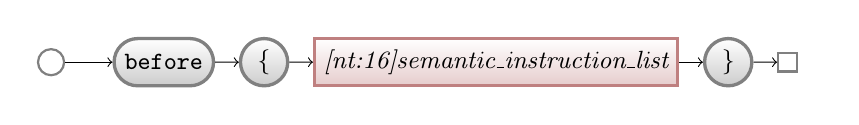
\begin{tikzpicture}
  \matrix[column sep=\ruleMatrixColumnSeparation, row sep=\ruleMatrixRowSeparation] {
    \node (P0start) [firstPoint] {}; & & \node (p0-2) [terminal] {before}; & \node (p0-3) [terminal] {\{}; & \node (p0-4) [nonterminal] {\nonTerminalSymbol{semantic\_instruction\_list}{16}}; & \node (p0-5) [terminal] {\}}; & \node (p0-6) [lastPoint] {}; & \\
  };
  \draw[->] (P0start) -- (p0-2) ;
  \draw[->] (p0-2) -- (p0-3) ;
  \draw[->] (p0-3) -- (p0-4) ;
  \draw[->] (p0-4) -- (p0-5) ;
  \draw[->] (p0-5) -- (p0-6) ;
\end{tikzpicture}

\ruleSubsection{galgas4ProgramDeclarations}{galgasProgramDeclarations}{139}

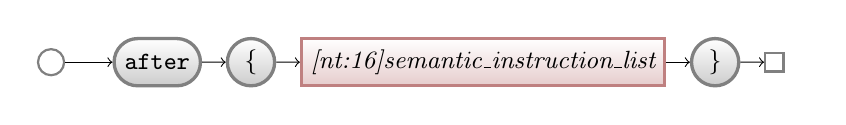
\begin{tikzpicture}
  \matrix[column sep=\ruleMatrixColumnSeparation, row sep=\ruleMatrixRowSeparation] {
    \node (P0start) [firstPoint] {}; & & \node (p0-2) [terminal] {after}; & \node (p0-3) [terminal] {\{}; & \node (p0-4) [nonterminal] {\nonTerminalSymbol{semantic\_instruction\_list}{16}}; & \node (p0-5) [terminal] {\}}; & \node (p0-6) [lastPoint] {}; & \\
  };
  \draw[->] (P0start) -- (p0-2) ;
  \draw[->] (p0-2) -- (p0-3) ;
  \draw[->] (p0-3) -- (p0-4) ;
  \draw[->] (p0-4) -- (p0-5) ;
  \draw[->] (p0-5) -- (p0-6) ;
\end{tikzpicture}

\ruleSubsection{galgas4ProgramDeclarations}{galgasProgramDeclarations}{154}

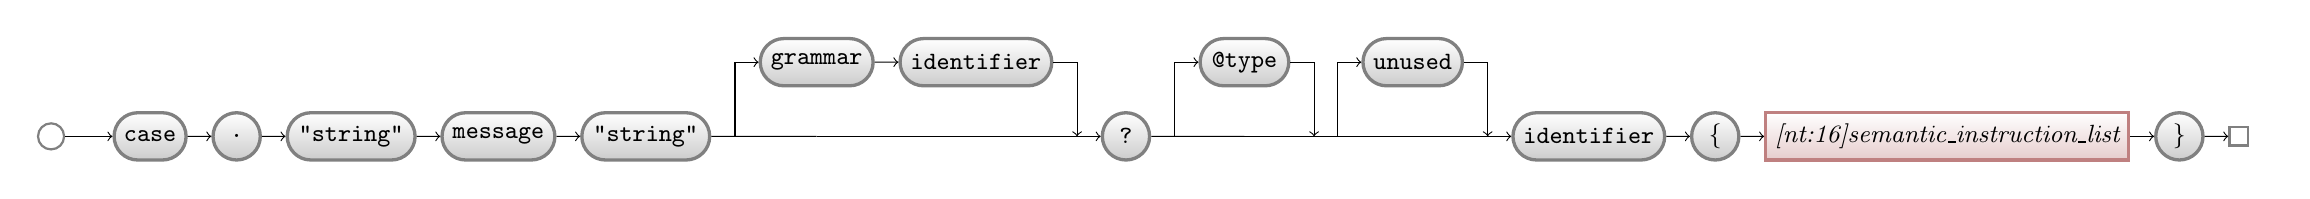
\begin{tikzpicture}
  \matrix[column sep=\ruleMatrixColumnSeparation, row sep=\ruleMatrixRowSeparation] {
    & & & & & & & & \node (p1-8) [terminal] {grammar}; & \node (p1-9) [terminal] {identifier}; & & & & \node (p1-13) [terminal] {@type}; & & & \node (p1-16) [terminal] {unused}; & \\
    \node (P0start) [firstPoint] {}; & & \node (p0-2) [terminal] {case}; & \node (p0-3) [terminal] {.}; & \node (p0-4) [terminal] {"string"}; & \node (p0-5) [terminal] {message}; & \node (p0-6) [terminal] {"string"}; & \node (p0-7) [point] {}; & \node (p0-8) [point] {}; & & \node (p0-10) [point] {}; & \node (p0-11) [terminal] {?}; & \node (p0-12) [point] {}; & \node (p0-13) [point] {}; & \node (p0-14) [point] {}; & \node (p0-15) [point] {}; & \node (p0-16) [point] {}; & \node (p0-17) [point] {}; & \node (p0-18) [terminal] {identifier}; & \node (p0-19) [terminal] {\{}; & \node (p0-20) [nonterminal] {\nonTerminalSymbol{semantic\_instruction\_list}{16}}; & \node (p0-21) [terminal] {\}}; & \node (p0-22) [lastPoint] {}; & \\
  };
  \draw[->] (P0start) -- (p0-2) ;
  \draw[->] (p0-2) -- (p0-3) ;
  \draw[->] (p0-3) -- (p0-4) ;
  \draw[->] (p0-4) -- (p0-5) ;
  \draw[->] (p0-5) -- (p0-6) ;
  \draw (p0-6) -- (p0-8) ;
  \draw[->] (p0-7) |- (p1-8) ;
  \draw[->] (p1-8) -- (p1-9) ;
  \draw (p0-8) -- (p0-10) ;
  \draw[->] (p1-9) -| (p0-10) ;
  \draw[->] (p0-10) -- (p0-11) ;
  \draw (p0-11) -- (p0-13) ;
  \draw[->] (p0-12) |- (p1-13) ;
  \draw (p0-13) -- (p0-14) ;
  \draw[->] (p1-13) -| (p0-14) ;
  \draw (p0-14) -- (p0-16) ;
  \draw[->] (p0-15) |- (p1-16) ;
  \draw (p0-16) -- (p0-17) ;
  \draw[->] (p1-16) -| (p0-17) ;
  \draw[->] (p0-17) -- (p0-18) ;
  \draw[->] (p0-18) -- (p0-19) ;
  \draw[->] (p0-19) -- (p0-20) ;
  \draw[->] (p0-20) -- (p0-21) ;
  \draw[->] (p0-21) -- (p0-22) ;
\end{tikzpicture}

\nonTerminalSection{expression}{6}

\ruleSubsection{galgas4ExpressionSyntax}{expression-is-as}{85}

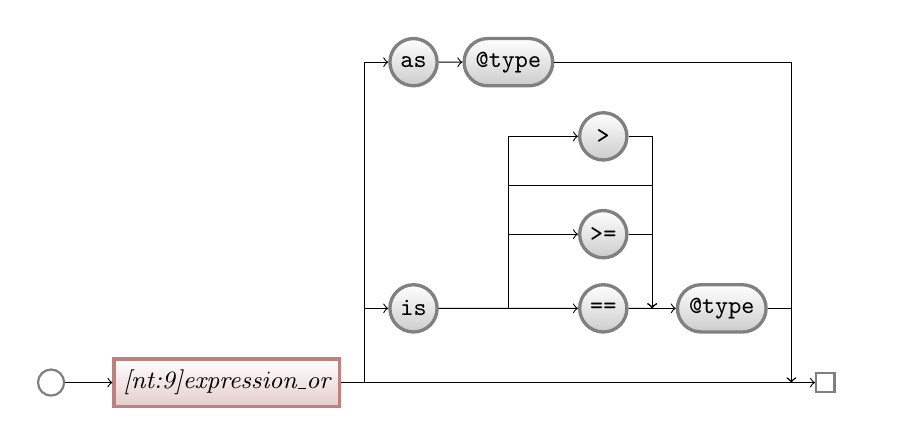
\begin{tikzpicture}
  \matrix[column sep=\ruleMatrixColumnSeparation, row sep=\ruleMatrixRowSeparation] {
    & & & & \node (p5-4) [terminal] {as}; & \node (p5-5) [terminal] {@type}; & \\
    & & & & & & \node (p4-6) [terminal] {>}; & \\
    & & & & & & \node (p3-6) [point] {}; & \\
    & & & & & & \node (p2-6) [terminal] {>=}; & \\
    & & & & \node (p1-4) [terminal] {is}; & \node (p1-5) [point] {}; & \node (p1-6) [terminal] {==}; & \node (p1-7) [point] {}; & \node (p1-8) [terminal] {@type}; & \\
    \node (P0start) [firstPoint] {}; & & \node (p0-2) [nonterminal] {\nonTerminalSymbol{expression\_or}{9}}; & \node (p0-3) [point] {}; & \node (p0-4) [point] {}; & & & & & \node (p0-9) [point] {}; & \node (p0-10) [lastPoint] {}; & \\
  };
  \draw[->] (P0start) -- (p0-2) ;
  \draw (p0-2) -- (p0-4) ;
  \draw[->] (p0-3) |- (p1-4) ;
  \draw[->] (p1-4) -- (p1-6) ;
  \draw[->] (p1-5) |- (p2-6) ;
  \draw (p1-5) |- (p3-6) ;
  \draw[->] (p1-5) |- (p4-6) ;
  \draw (p1-6) -- (p1-7) ;
  \draw[->] (p2-6) -| (p1-7) ;
  \draw[->] (p3-6) -| (p1-7) ;
  \draw[->] (p4-6) -| (p1-7) ;
  \draw[->] (p1-7) -- (p1-8) ;
  \draw[->] (p0-3) |- (p5-4) ;
  \draw[->] (p5-4) -- (p5-5) ;
  \draw (p0-4) -- (p0-9) ;
  \draw[->] (p1-8) -| (p0-9) ;
  \draw[->] (p5-5) -| (p0-9) ;
  \draw[->] (p0-9) -- (p0-10) ;
\end{tikzpicture}

\nonTerminalSection{expression\_and}{10}

\ruleSubsection{galgas4ExpressionSyntax}{expression-and}{55}

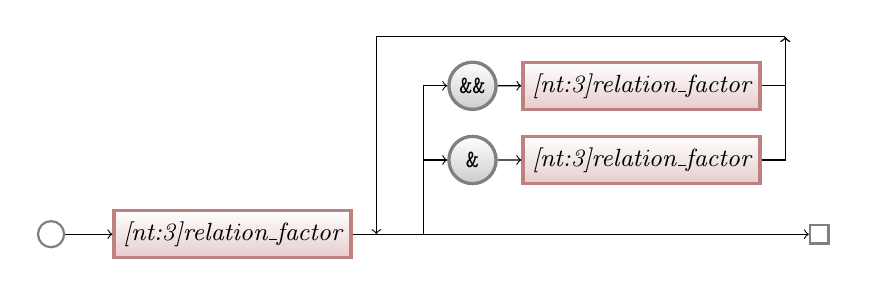
\begin{tikzpicture}
  \matrix[column sep=\ruleMatrixColumnSeparation, row sep=\ruleMatrixRowSeparation] {
    & & & & & & & & \node (p3-8) [point] {}; & \\
    & & & & & & \node (p2-6) [terminal] {\&\&}; & \node (p2-7) [nonterminal] {\nonTerminalSymbol{relation\_factor}{3}}; & \\
    & & & & & & \node (p1-6) [terminal] {\&}; & \node (p1-7) [nonterminal] {\nonTerminalSymbol{relation\_factor}{3}}; & \\
    \node (P0start) [firstPoint] {}; & & \node (p0-2) [nonterminal] {\nonTerminalSymbol{relation\_factor}{3}}; & \node (p0-3) [point] {}; & \node (p0-4) [point] {}; & \node (p0-5) [point] {}; & & & & \node (p0-9) [lastPoint] {}; & \\
  };
  \draw[->] (P0start) -- (p0-2) ;
  \draw (p0-2) -- (p0-4) ;
  \draw[->] (p0-5) |- (p1-6) ;
  \draw[->] (p1-6) -- (p1-7) ;
  \draw[->] (p0-5) |- (p2-6) ;
  \draw[->] (p2-6) -- (p2-7) ;
  \draw[->] (p3-8) -| (p0-3) ;
  \draw[->] (p1-7) -| (p3-8) ;
  \draw[->] (p2-7) -| (p3-8) ;
  \draw[->] (p0-4) -- (p0-9) ;
\end{tikzpicture}

\nonTerminalSection{expression\_or}{9}

\ruleSubsection{galgas4ExpressionSyntax}{expression-or}{97}

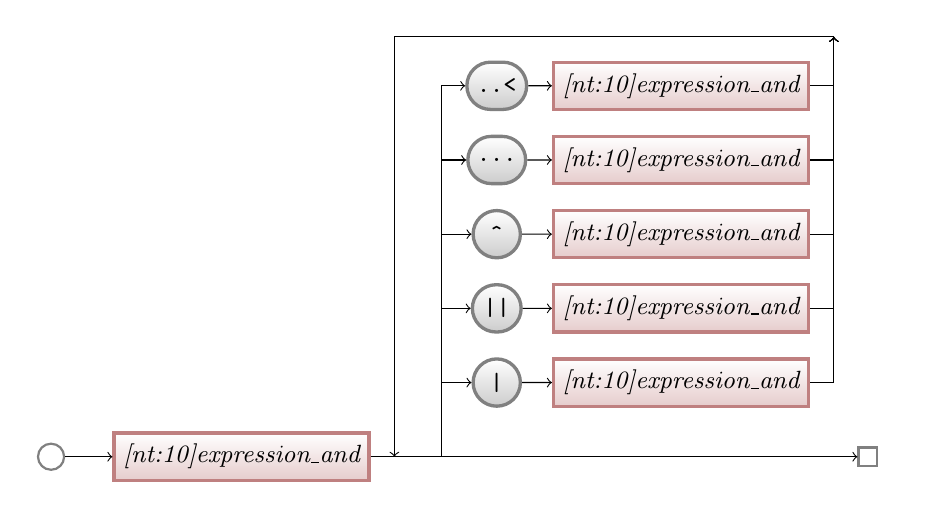
\begin{tikzpicture}
  \matrix[column sep=\ruleMatrixColumnSeparation, row sep=\ruleMatrixRowSeparation] {
    & & & & & & & & \node (p6-8) [point] {}; & \\
    & & & & & & \node (p5-6) [terminal] {..<}; & \node (p5-7) [nonterminal] {\nonTerminalSymbol{expression\_and}{10}}; & \\
    & & & & & & \node (p4-6) [terminal] {...}; & \node (p4-7) [nonterminal] {\nonTerminalSymbol{expression\_and}{10}}; & \\
    & & & & & & \node (p3-6) [terminal] {\verb=^=}; & \node (p3-7) [nonterminal] {\nonTerminalSymbol{expression\_and}{10}}; & \\
    & & & & & & \node (p2-6) [terminal] {||}; & \node (p2-7) [nonterminal] {\nonTerminalSymbol{expression\_and}{10}}; & \\
    & & & & & & \node (p1-6) [terminal] {|}; & \node (p1-7) [nonterminal] {\nonTerminalSymbol{expression\_and}{10}}; & \\
    \node (P0start) [firstPoint] {}; & & \node (p0-2) [nonterminal] {\nonTerminalSymbol{expression\_and}{10}}; & \node (p0-3) [point] {}; & \node (p0-4) [point] {}; & \node (p0-5) [point] {}; & & & & \node (p0-9) [lastPoint] {}; & \\
  };
  \draw[->] (P0start) -- (p0-2) ;
  \draw (p0-2) -- (p0-4) ;
  \draw[->] (p0-5) |- (p1-6) ;
  \draw[->] (p1-6) -- (p1-7) ;
  \draw[->] (p0-5) |- (p2-6) ;
  \draw[->] (p2-6) -- (p2-7) ;
  \draw[->] (p0-5) |- (p3-6) ;
  \draw[->] (p3-6) -- (p3-7) ;
  \draw[->] (p0-5) |- (p4-6) ;
  \draw[->] (p4-6) -- (p4-7) ;
  \draw[->] (p0-5) |- (p5-6) ;
  \draw[->] (p5-6) -- (p5-7) ;
  \draw[->] (p6-8) -| (p0-3) ;
  \draw[->] (p1-7) -| (p6-8) ;
  \draw[->] (p2-7) -| (p6-8) ;
  \draw[->] (p3-7) -| (p6-8) ;
  \draw[->] (p4-7) -| (p6-8) ;
  \draw[->] (p5-7) -| (p6-8) ;
  \draw[->] (p0-4) -- (p0-9) ;
\end{tikzpicture}

\nonTerminalSection{externtype\_constructor}{37}

\ruleSubsection{galgas4DeclarationsSyntax}{type-extern}{247}

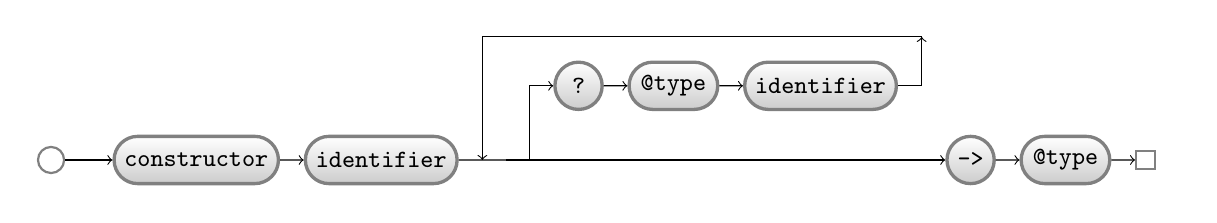
\begin{tikzpicture}
  \matrix[column sep=\ruleMatrixColumnSeparation, row sep=\ruleMatrixRowSeparation] {
    & & & & & & & & & & \node (p2-10) [point] {}; & \\
    & & & & & & & \node (p1-7) [terminal] {?}; & \node (p1-8) [terminal] {@type}; & \node (p1-9) [terminal] {identifier}; & \\
    \node (P0start) [firstPoint] {}; & & \node (p0-2) [terminal] {constructor}; & \node (p0-3) [terminal] {identifier}; & \node (p0-4) [point] {}; & \node (p0-5) [point] {}; & \node (p0-6) [point] {}; & & & & & \node (p0-11) [terminal] {->}; & \node (p0-12) [terminal] {@type}; & \node (p0-13) [lastPoint] {}; & \\
  };
  \draw[->] (P0start) -- (p0-2) ;
  \draw[->] (p0-2) -- (p0-3) ;
  \draw (p0-3) -- (p0-5) ;
  \draw[->] (p0-6) |- (p1-7) ;
  \draw[->] (p1-7) -- (p1-8) ;
  \draw[->] (p1-8) -- (p1-9) ;
  \draw[->] (p2-10) -| (p0-4) ;
  \draw[->] (p1-9) -| (p2-10) ;
  \draw[->] (p0-5) -- (p0-11) ;
  \draw[->] (p0-11) -- (p0-12) ;
  \draw[->] (p0-12) -- (p0-13) ;
\end{tikzpicture}

\nonTerminalSection{externtype\_cpp\_classdeclaration}{36}

\ruleSubsection{galgas4DeclarationsSyntax}{type-extern}{234}

\begin{tikzpicture}
  \matrix[column sep=\ruleMatrixColumnSeparation, row sep=\ruleMatrixRowSeparation] {
    & & & & & & & \node (p2-7) [point] {}; & \\
    & & & & & & \node (p1-6) [terminal] {"string"}; & \\
    \node (P0start) [firstPoint] {}; & & \node (p0-2) [terminal] {\{}; & \node (p0-3) [point] {}; & \node (p0-4) [point] {}; & \node (p0-5) [point] {}; & & & \node (p0-8) [terminal] {\}}; & \node (p0-9) [lastPoint] {}; & \\
  };
  \draw[->] (P0start) -- (p0-2) ;
  \draw (p0-2) -- (p0-4) ;
  \draw[->] (p0-5) |- (p1-6) ;
  \draw[->] (p2-7) -| (p0-3) ;
  \draw[->] (p1-6) -| (p2-7) ;
  \draw[->] (p0-4) -- (p0-8) ;
  \draw[->] (p0-8) -- (p0-9) ;
\end{tikzpicture}

\nonTerminalSection{externtype\_cpp\_predeclaration}{35}

\ruleSubsection{galgas4DeclarationsSyntax}{type-extern}{221}

\begin{tikzpicture}
  \matrix[column sep=\ruleMatrixColumnSeparation, row sep=\ruleMatrixRowSeparation] {
    & & & & & & & \node (p2-7) [point] {}; & \\
    & & & & & & \node (p1-6) [terminal] {"string"}; & \\
    \node (P0start) [firstPoint] {}; & & \node (p0-2) [terminal] {\{}; & \node (p0-3) [point] {}; & \node (p0-4) [point] {}; & \node (p0-5) [point] {}; & & & \node (p0-8) [terminal] {\}}; & \node (p0-9) [lastPoint] {}; & \\
  };
  \draw[->] (P0start) -- (p0-2) ;
  \draw (p0-2) -- (p0-4) ;
  \draw[->] (p0-5) |- (p1-6) ;
  \draw[->] (p2-7) -| (p0-3) ;
  \draw[->] (p1-6) -| (p2-7) ;
  \draw[->] (p0-4) -- (p0-8) ;
  \draw[->] (p0-8) -- (p0-9) ;
\end{tikzpicture}

\nonTerminalSection{externtype\_getter}{38}

\ruleSubsection{galgas4DeclarationsSyntax}{type-extern}{265}

\begin{tikzpicture}
  \matrix[column sep=\ruleMatrixColumnSeparation, row sep=\ruleMatrixRowSeparation] {
    & & & & & & & & & & \node (p2-10) [point] {}; & \\
    & & & & & & & \node (p1-7) [terminal] {?}; & \node (p1-8) [terminal] {@type}; & \node (p1-9) [terminal] {identifier}; & \\
    \node (P0start) [firstPoint] {}; & & \node (p0-2) [terminal] {getter}; & \node (p0-3) [terminal] {identifier}; & \node (p0-4) [point] {}; & \node (p0-5) [point] {}; & \node (p0-6) [point] {}; & & & & & \node (p0-11) [terminal] {->}; & \node (p0-12) [terminal] {@type}; & \node (p0-13) [lastPoint] {}; & \\
  };
  \draw[->] (P0start) -- (p0-2) ;
  \draw[->] (p0-2) -- (p0-3) ;
  \draw (p0-3) -- (p0-5) ;
  \draw[->] (p0-6) |- (p1-7) ;
  \draw[->] (p1-7) -- (p1-8) ;
  \draw[->] (p1-8) -- (p1-9) ;
  \draw[->] (p2-10) -| (p0-4) ;
  \draw[->] (p1-9) -| (p2-10) ;
  \draw[->] (p0-5) -- (p0-11) ;
  \draw[->] (p0-11) -- (p0-12) ;
  \draw[->] (p0-12) -- (p0-13) ;
\end{tikzpicture}

\nonTerminalSection{externtype\_method}{40}

\ruleSubsection{galgas4DeclarationsSyntax}{type-extern}{292}

\begin{tikzpicture}
  \matrix[column sep=\ruleMatrixColumnSeparation, row sep=\ruleMatrixRowSeparation] {
    \node (P0start) [firstPoint] {}; & & \node (p0-2) [terminal] {method}; & \node (p0-3) [terminal] {identifier}; & \node (p0-4) [nonterminal] {\nonTerminalSymbol{formal\_parameter\_list}{11}}; & \node (p0-5) [lastPoint] {}; & \\
  };
  \draw[->] (P0start) -- (p0-2) ;
  \draw[->] (p0-2) -- (p0-3) ;
  \draw[->] (p0-3) -- (p0-4) ;
  \draw[->] (p0-4) -- (p0-5) ;
\end{tikzpicture}

\nonTerminalSection{externtype\_setter}{39}

\ruleSubsection{galgas4DeclarationsSyntax}{type-extern}{283}

\begin{tikzpicture}
  \matrix[column sep=\ruleMatrixColumnSeparation, row sep=\ruleMatrixRowSeparation] {
    \node (P0start) [firstPoint] {}; & & \node (p0-2) [terminal] {setter}; & \node (p0-3) [terminal] {identifier}; & \node (p0-4) [nonterminal] {\nonTerminalSymbol{formal\_parameter\_list}{11}}; & \node (p0-5) [lastPoint] {}; & \\
  };
  \draw[->] (P0start) -- (p0-2) ;
  \draw[->] (p0-2) -- (p0-3) ;
  \draw[->] (p0-3) -- (p0-4) ;
  \draw[->] (p0-4) -- (p0-5) ;
\end{tikzpicture}

\nonTerminalSection{factor}{1}

\ruleSubsection{galgas4ExpressionSyntax}{expression-unary-plus}{35}

\begin{tikzpicture}
  \matrix[column sep=\ruleMatrixColumnSeparation, row sep=\ruleMatrixRowSeparation] {
    \node (P0start) [firstPoint] {}; & & \node (p0-2) [terminal] {+}; & \node (p0-3) [nonterminal] {\nonTerminalSymbol{factor}{1}}; & \node (p0-4) [lastPoint] {}; & \\
  };
  \draw[->] (P0start) -- (p0-2) ;
  \draw[->] (p0-2) -- (p0-3) ;
  \draw[->] (p0-3) -- (p0-4) ;
\end{tikzpicture}

\ruleSubsection{galgas4ExpressionSyntax}{expression-unary-minus}{35}

\begin{tikzpicture}
  \matrix[column sep=\ruleMatrixColumnSeparation, row sep=\ruleMatrixRowSeparation] {
    \node (P0start) [firstPoint] {}; & & \node (p0-2) [terminal] {-}; & \node (p0-3) [nonterminal] {\nonTerminalSymbol{factor}{1}}; & \node (p0-4) [lastPoint] {}; & \\
  };
  \draw[->] (P0start) -- (p0-2) ;
  \draw[->] (p0-2) -- (p0-3) ;
  \draw[->] (p0-3) -- (p0-4) ;
\end{tikzpicture}

\ruleSubsection{galgas4ExpressionSyntax}{expression-property-access}{39}

\begin{tikzpicture}
  \matrix[column sep=\ruleMatrixColumnSeparation, row sep=\ruleMatrixRowSeparation] {
    & & & & & & & & \node (p2-8) [point] {}; & \\
    & & & & & & \node (p1-6) [terminal] {.}; & \node (p1-7) [terminal] {identifier}; & \\
    \node (P0start) [firstPoint] {}; & & \node (p0-2) [nonterminal] {\nonTerminalSymbol{primary}{0}}; & \node (p0-3) [point] {}; & \node (p0-4) [point] {}; & \node (p0-5) [point] {}; & & & & \node (p0-9) [lastPoint] {}; & \\
  };
  \draw[->] (P0start) -- (p0-2) ;
  \draw (p0-2) -- (p0-4) ;
  \draw[->] (p0-5) |- (p1-6) ;
  \draw[->] (p1-6) -- (p1-7) ;
  \draw[->] (p2-8) -| (p0-3) ;
  \draw[->] (p1-7) -| (p2-8) ;
  \draw[->] (p0-4) -- (p0-9) ;
\end{tikzpicture}

\ruleSubsection{galgas4ExpressionSyntax}{expression-not}{35}

\begin{tikzpicture}
  \matrix[column sep=\ruleMatrixColumnSeparation, row sep=\ruleMatrixRowSeparation] {
    \node (P0start) [firstPoint] {}; & & \node (p0-2) [terminal] {not}; & \node (p0-3) [nonterminal] {\nonTerminalSymbol{factor}{1}}; & \node (p0-4) [lastPoint] {}; & \\
  };
  \draw[->] (P0start) -- (p0-2) ;
  \draw[->] (p0-2) -- (p0-3) ;
  \draw[->] (p0-3) -- (p0-4) ;
\end{tikzpicture}

\ruleSubsection{galgas4ExpressionSyntax}{expression-tilde}{35}

\begin{tikzpicture}
  \matrix[column sep=\ruleMatrixColumnSeparation, row sep=\ruleMatrixRowSeparation] {
    \node (P0start) [firstPoint] {}; & & \node (p0-2) [terminal] {$\sim$}; & \node (p0-3) [nonterminal] {\nonTerminalSymbol{factor}{1}}; & \node (p0-4) [lastPoint] {}; & \\
  };
  \draw[->] (P0start) -- (p0-2) ;
  \draw[->] (p0-2) -- (p0-3) ;
  \draw[->] (p0-3) -- (p0-4) ;
\end{tikzpicture}

\ruleSubsection{galgas4ExpressionSyntax}{expression-unary-wrapping-minus}{35}

\begin{tikzpicture}
  \matrix[column sep=\ruleMatrixColumnSeparation, row sep=\ruleMatrixRowSeparation] {
    \node (P0start) [firstPoint] {}; & & \node (p0-2) [terminal] {\&-}; & \node (p0-3) [nonterminal] {\nonTerminalSymbol{factor}{1}}; & \node (p0-4) [lastPoint] {}; & \\
  };
  \draw[->] (P0start) -- (p0-2) ;
  \draw[->] (p0-2) -- (p0-3) ;
  \draw[->] (p0-3) -- (p0-4) ;
\end{tikzpicture}

\nonTerminalSection{filewrapper\_binary\_files}{33}

\ruleSubsection{galgas4DeclarationsSyntax}{galgasDeclarationsSyntax}{398}

\begin{tikzpicture}
  \matrix[column sep=\ruleMatrixColumnSeparation, row sep=\ruleMatrixRowSeparation] {
    & & & & & & & & \node (p3-8) [point] {}; & \\
    & & & & & & & \node (p2-7) [terminal] {,}; & \\
    & & & & \node (p1-4) [point] {}; & \node (p1-5) [terminal] {"string"}; & \node (p1-6) [point] {}; & \\
    \node (P0start) [firstPoint] {}; & & \node (p0-2) [terminal] {\{}; & \node (p0-3) [point] {}; & \node (p0-4) [point] {}; & & & & & \node (p0-9) [point] {}; & \node (p0-10) [terminal] {\}}; & \node (p0-11) [lastPoint] {}; & \\
  };
  \draw[->] (P0start) -- (p0-2) ;
  \draw (p0-2) -- (p0-4) ;
  \draw[->] (p0-3) |- (p1-5) ;
  \draw[->] (p1-6) |- (p2-7) ;
  \draw[->] (p3-8) -| (p1-4) ;
  \draw[->] (p2-7) -| (p3-8) ;
  \draw (p0-4) -- (p0-9) ;
  \draw[->] (p1-5) -| (p0-9) ;
  \draw[->] (p0-9) -- (p0-10) ;
  \draw[->] (p0-10) -- (p0-11) ;
\end{tikzpicture}

\nonTerminalSection{filewrapper\_templates}{34}

\ruleSubsection{galgas4DeclarationsSyntax}{galgasDeclarationsSyntax}{415}

\begin{tikzpicture}
  \matrix[column sep=\ruleMatrixColumnSeparation, row sep=\ruleMatrixRowSeparation] {
    & & & & & & & & & & & & & & & & & & & \node (p5-19) [point] {}; & \\
    & & & & & & & & & & & & & & & & & & \node (p4-18) [point] {}; & \\
    & & & & & & & & & & & & & & & \node (p3-15) [terminal] {unused}; & \\
    & & & & & & & & & & & & \node (p2-12) [terminal] {?}; & \node (p2-13) [terminal] {@type}; & \node (p2-14) [point] {}; & \node (p2-15) [point] {}; & \node (p2-16) [point] {}; & \node (p2-17) [terminal] {identifier}; & \\
    & & & & & & \node (p1-6) [terminal] {template}; & \node (p1-7) [terminal] {identifier}; & \node (p1-8) [terminal] {"string"}; & \node (p1-9) [point] {}; & \node (p1-10) [point] {}; & \node (p1-11) [point] {}; & \\
    \node (P0start) [firstPoint] {}; & & \node (p0-2) [terminal] {\{}; & \node (p0-3) [point] {}; & \node (p0-4) [point] {}; & \node (p0-5) [point] {}; & & & & & & & & & & & & & & & \node (p0-20) [terminal] {\}}; & \node (p0-21) [lastPoint] {}; & \\
  };
  \draw[->] (P0start) -- (p0-2) ;
  \draw (p0-2) -- (p0-4) ;
  \draw[->] (p0-5) |- (p1-6) ;
  \draw[->] (p1-6) -- (p1-7) ;
  \draw[->] (p1-7) -- (p1-8) ;
  \draw (p1-8) -- (p1-10) ;
  \draw[->] (p1-11) |- (p2-12) ;
  \draw[->] (p2-12) -- (p2-13) ;
  \draw (p2-13) -- (p2-15) ;
  \draw[->] (p2-14) |- (p3-15) ;
  \draw (p2-15) -- (p2-16) ;
  \draw[->] (p3-15) -| (p2-16) ;
  \draw[->] (p2-16) -- (p2-17) ;
  \draw[->] (p4-18) -| (p1-9) ;
  \draw[->] (p2-17) -| (p4-18) ;
  \draw[->] (p5-19) -| (p0-3) ;
  \draw[->] (p1-10) -| (p5-19) ;
  \draw[->] (p0-4) -- (p0-20) ;
  \draw[->] (p0-20) -- (p0-21) ;
\end{tikzpicture}

\nonTerminalSection{filewrapper\_text\_files}{32}

\ruleSubsection{galgas4DeclarationsSyntax}{galgasDeclarationsSyntax}{381}

\begin{tikzpicture}
  \matrix[column sep=\ruleMatrixColumnSeparation, row sep=\ruleMatrixRowSeparation] {
    & & & & & & & & \node (p3-8) [point] {}; & \\
    & & & & & & & \node (p2-7) [terminal] {,}; & \\
    & & & & \node (p1-4) [point] {}; & \node (p1-5) [terminal] {"string"}; & \node (p1-6) [point] {}; & \\
    \node (P0start) [firstPoint] {}; & & \node (p0-2) [terminal] {\{}; & \node (p0-3) [point] {}; & \node (p0-4) [point] {}; & & & & & \node (p0-9) [point] {}; & \node (p0-10) [terminal] {\}}; & \node (p0-11) [lastPoint] {}; & \\
  };
  \draw[->] (P0start) -- (p0-2) ;
  \draw (p0-2) -- (p0-4) ;
  \draw[->] (p0-3) |- (p1-5) ;
  \draw[->] (p1-6) |- (p2-7) ;
  \draw[->] (p3-8) -| (p1-4) ;
  \draw[->] (p2-7) -| (p3-8) ;
  \draw (p0-4) -- (p0-9) ;
  \draw[->] (p1-5) -| (p0-9) ;
  \draw[->] (p0-9) -- (p0-10) ;
  \draw[->] (p0-10) -- (p0-11) ;
\end{tikzpicture}

\nonTerminalSection{for\_instruction\_element}{24}

\ruleSubsection{galgas4InstructionsSyntax}{instruction-for}{293}

\begin{tikzpicture}
  \matrix[column sep=\ruleMatrixColumnSeparation, row sep=\ruleMatrixRowSeparation] {
    \node (P0start) [firstPoint] {}; & & \node (p0-2) [terminal] {literalInt}; & \node (p0-3) [terminal] {*}; & \node (p0-4) [lastPoint] {}; & \\
  };
  \draw[->] (P0start) -- (p0-2) ;
  \draw[->] (p0-2) -- (p0-3) ;
  \draw[->] (p0-3) -- (p0-4) ;
\end{tikzpicture}

\ruleSubsection{galgas4InstructionsSyntax}{instruction-for}{308}

\begin{tikzpicture}
  \matrix[column sep=\ruleMatrixColumnSeparation, row sep=\ruleMatrixRowSeparation] {
    & & & & & & & \node (p2-7) [terminal] {unused}; & \\
    & & & \node (p1-3) [terminal] {@type}; & & & \node (p1-6) [point] {}; & \node (p1-7) [point] {}; & \node (p1-8) [point] {}; & \node (p1-9) [terminal] {identifier}; & \\
    \node (P0start) [firstPoint] {}; & & \node (p0-2) [point] {}; & \node (p0-3) [point] {}; & \node (p0-4) [point] {}; & \node (p0-5) [point] {}; & \node (p0-6) [terminal] {*}; & & & & \node (p0-10) [point] {}; & \node (p0-11) [lastPoint] {}; & \\
  };
  \draw (P0start) -- (p0-3) ;
  \draw[->] (p0-2) |- (p1-3) ;
  \draw (p0-3) -- (p0-4) ;
  \draw[->] (p1-3) -| (p0-4) ;
  \draw[->] (p0-4) -- (p0-6) ;
  \draw (p0-5) |- (p1-7) ;
  \draw[->] (p1-6) |- (p2-7) ;
  \draw (p1-7) -- (p1-8) ;
  \draw[->] (p2-7) -| (p1-8) ;
  \draw[->] (p1-8) -- (p1-9) ;
  \draw (p0-6) -- (p0-10) ;
  \draw[->] (p1-9) -| (p0-10) ;
  \draw[->] (p0-10) -- (p0-11) ;
\end{tikzpicture}

\nonTerminalSection{for\_instruction\_enumerated\_object}{25}

\ruleSubsection{galgas4InstructionsSyntax}{instruction-for}{333}

\begin{tikzpicture}
  \matrix[column sep=\ruleMatrixColumnSeparation, row sep=\ruleMatrixRowSeparation] {
    & & & & & & \node (p1-6) [point] {}; & \\
    \node (P0start) [firstPoint] {}; & & \node (p0-2) [terminal] {(}; & \node (p0-3) [point] {}; & \node (p0-4) [nonterminal] {\nonTerminalSymbol{for\_instruction\_element}{24}}; & \node (p0-5) [point] {}; & & \node (p0-7) [terminal] {)}; & \node (p0-8) [terminal] {in}; & \node (p0-9) [nonterminal] {\nonTerminalSymbol{expression}{6}}; & \node (p0-10) [lastPoint] {}; & \\
  };
  \draw[->] (P0start) -- (p0-2) ;
  \draw[->] (p0-2) -- (p0-4) ;
  \draw[->] (p1-6) -| (p0-3) ;
  \draw[->] (p0-5) -| (p1-6) ;
  \draw[->] (p0-4) -- (p0-7) ;
  \draw[->] (p0-7) -- (p0-8) ;
  \draw[->] (p0-8) -- (p0-9) ;
  \draw[->] (p0-9) -- (p0-10) ;
\end{tikzpicture}

\ruleSubsection{galgas4InstructionsSyntax}{instruction-for}{354}

\begin{tikzpicture}
  \matrix[column sep=\ruleMatrixColumnSeparation, row sep=\ruleMatrixRowSeparation] {
    & & & \node (p1-3) [terminal] {@type}; & & & \node (p1-6) [terminal] {identifier}; & \\
    \node (P0start) [firstPoint] {}; & & \node (p0-2) [point] {}; & \node (p0-3) [point] {}; & \node (p0-4) [point] {}; & \node (p0-5) [point] {}; & \node (p0-6) [terminal] {*}; & \node (p0-7) [point] {}; & \node (p0-8) [terminal] {in}; & \node (p0-9) [nonterminal] {\nonTerminalSymbol{expression}{6}}; & \node (p0-10) [lastPoint] {}; & \\
  };
  \draw (P0start) -- (p0-3) ;
  \draw[->] (p0-2) |- (p1-3) ;
  \draw (p0-3) -- (p0-4) ;
  \draw[->] (p1-3) -| (p0-4) ;
  \draw[->] (p0-4) -- (p0-6) ;
  \draw[->] (p0-5) |- (p1-6) ;
  \draw (p0-6) -- (p0-7) ;
  \draw[->] (p1-6) -| (p0-7) ;
  \draw[->] (p0-7) -- (p0-8) ;
  \draw[->] (p0-8) -- (p0-9) ;
  \draw[->] (p0-9) -- (p0-10) ;
\end{tikzpicture}

\ruleSubsection{galgas4InstructionsSyntax}{instruction-for}{380}

\begin{tikzpicture}
  \matrix[column sep=\ruleMatrixColumnSeparation, row sep=\ruleMatrixRowSeparation] {
    & & & & & \node (p1-5) [terminal] {identifier}; & \\
    \node (P0start) [firstPoint] {}; & & \node (p0-2) [terminal] {(}; & \node (p0-3) [terminal] {)}; & \node (p0-4) [point] {}; & \node (p0-5) [point] {}; & \node (p0-6) [point] {}; & \node (p0-7) [terminal] {in}; & \node (p0-8) [nonterminal] {\nonTerminalSymbol{expression}{6}}; & \node (p0-9) [lastPoint] {}; & \\
  };
  \draw[->] (P0start) -- (p0-2) ;
  \draw[->] (p0-2) -- (p0-3) ;
  \draw (p0-3) -- (p0-5) ;
  \draw[->] (p0-4) |- (p1-5) ;
  \draw (p0-5) -- (p0-6) ;
  \draw[->] (p1-5) -| (p0-6) ;
  \draw[->] (p0-6) -- (p0-7) ;
  \draw[->] (p0-7) -- (p0-8) ;
  \draw[->] (p0-8) -- (p0-9) ;
\end{tikzpicture}

\nonTerminalSection{formal\_input\_parameter\_list}{14}

\ruleSubsection{galgas4ParameterArgumentSyntax}{galgasParameterArgumentSyntax}{468}

\begin{tikzpicture}
  \matrix[column sep=\ruleMatrixColumnSeparation, row sep=\ruleMatrixRowSeparation] {
    & & & & & & & & & & & & & & & \node (p3-15) [point] {}; & \\
    & & & & & & & & \node (p2-8) [terminal] {let}; & & & & \node (p2-12) [terminal] {unused}; & \\
    & & & & & & \node (p1-6) [terminal] {?}; & \node (p1-7) [point] {}; & \node (p1-8) [point] {}; & \node (p1-9) [point] {}; & \node (p1-10) [terminal] {@type}; & \node (p1-11) [point] {}; & \node (p1-12) [point] {}; & \node (p1-13) [point] {}; & \node (p1-14) [terminal] {identifier}; & \\
    \node (P0start) [firstPoint] {}; & & \node (p0-2) [terminal] {(}; & \node (p0-3) [point] {}; & \node (p0-4) [point] {}; & \node (p0-5) [point] {}; & & & & & & & & & & & \node (p0-16) [terminal] {)}; & \node (p0-17) [lastPoint] {}; & \\
  };
  \draw[->] (P0start) -- (p0-2) ;
  \draw (p0-2) -- (p0-4) ;
  \draw[->] (p0-5) |- (p1-6) ;
  \draw (p1-6) -- (p1-8) ;
  \draw[->] (p1-7) |- (p2-8) ;
  \draw (p1-8) -- (p1-9) ;
  \draw[->] (p2-8) -| (p1-9) ;
  \draw[->] (p1-9) -- (p1-10) ;
  \draw (p1-10) -- (p1-12) ;
  \draw[->] (p1-11) |- (p2-12) ;
  \draw (p1-12) -- (p1-13) ;
  \draw[->] (p2-12) -| (p1-13) ;
  \draw[->] (p1-13) -- (p1-14) ;
  \draw[->] (p3-15) -| (p0-3) ;
  \draw[->] (p1-14) -| (p3-15) ;
  \draw[->] (p0-4) -- (p0-16) ;
  \draw[->] (p0-16) -- (p0-17) ;
\end{tikzpicture}

\nonTerminalSection{formal\_parameter\_list}{11}

\ruleSubsection{galgas4ParameterArgumentSyntax}{galgasParameterArgumentSyntax}{265}

\begin{tikzpicture}
  \matrix[column sep=\ruleMatrixColumnSeparation, row sep=\ruleMatrixRowSeparation] {
    & & & & & & & & & & & & & & & \node (p5-15) [point] {}; & \\
    & & & & & & & \node (p4-7) [terminal] {!}; & \\
    & & & & & & & \node (p3-7) [terminal] {?!}; & \\
    & & & & & & & \node (p2-7) [terminal] {?}; & \node (p2-8) [terminal] {let}; & & & & \node (p2-12) [terminal] {unused}; & \\
    & & & & & & \node (p1-6) [point] {}; & \node (p1-7) [terminal] {?}; & & \node (p1-9) [point] {}; & \node (p1-10) [terminal] {@type}; & \node (p1-11) [point] {}; & \node (p1-12) [point] {}; & \node (p1-13) [point] {}; & \node (p1-14) [terminal] {identifier}; & \\
    \node (P0start) [firstPoint] {}; & & \node (p0-2) [terminal] {(}; & \node (p0-3) [point] {}; & \node (p0-4) [point] {}; & \node (p0-5) [point] {}; & & & & & & & & & & & \node (p0-16) [terminal] {)}; & \node (p0-17) [lastPoint] {}; & \\
  };
  \draw[->] (P0start) -- (p0-2) ;
  \draw (p0-2) -- (p0-4) ;
  \draw[->] (p0-5) |- (p1-7) ;
  \draw[->] (p1-6) |- (p2-7) ;
  \draw[->] (p2-7) -- (p2-8) ;
  \draw[->] (p1-6) |- (p3-7) ;
  \draw[->] (p1-6) |- (p4-7) ;
  \draw (p1-7) -- (p1-9) ;
  \draw[->] (p2-8) -| (p1-9) ;
  \draw[->] (p3-7) -| (p1-9) ;
  \draw[->] (p4-7) -| (p1-9) ;
  \draw[->] (p1-9) -- (p1-10) ;
  \draw (p1-10) -- (p1-12) ;
  \draw[->] (p1-11) |- (p2-12) ;
  \draw (p1-12) -- (p1-13) ;
  \draw[->] (p2-12) -| (p1-13) ;
  \draw[->] (p1-13) -- (p1-14) ;
  \draw[->] (p5-15) -| (p0-3) ;
  \draw[->] (p1-14) -| (p5-15) ;
  \draw[->] (p0-4) -- (p0-16) ;
  \draw[->] (p0-16) -- (p0-17) ;
\end{tikzpicture}

\nonTerminalSection{grammar\_instruction\_core}{26}

\ruleSubsection{galgas4InstructionsSyntax}{instruction-grammar}{271}

\begin{tikzpicture}
  \matrix[column sep=\ruleMatrixColumnSeparation, row sep=\ruleMatrixRowSeparation] {
    & & & & & \node (p1-5) [terminal] {:>}; & \node (p1-6) [nonterminal] {\nonTerminalSymbol{syntax\_directed\_translation\_result}{18}}; & \\
    \node (P0start) [firstPoint] {}; & & \node (p0-2) [terminal] {in}; & \node (p0-3) [nonterminal] {\nonTerminalSymbol{expression}{6}}; & \node (p0-4) [point] {}; & \node (p0-5) [point] {}; & & \node (p0-7) [point] {}; & \node (p0-8) [lastPoint] {}; & \\
  };
  \draw[->] (P0start) -- (p0-2) ;
  \draw[->] (p0-2) -- (p0-3) ;
  \draw (p0-3) -- (p0-5) ;
  \draw[->] (p0-4) |- (p1-5) ;
  \draw[->] (p1-5) -- (p1-6) ;
  \draw (p0-5) -- (p0-7) ;
  \draw[->] (p1-6) -| (p0-7) ;
  \draw[->] (p0-7) -- (p0-8) ;
\end{tikzpicture}

\ruleSubsection{galgas4InstructionsSyntax}{instruction-grammar}{300}

\begin{tikzpicture}
  \matrix[column sep=\ruleMatrixColumnSeparation, row sep=\ruleMatrixRowSeparation] {
    & & & & & & & \node (p1-7) [terminal] {:>}; & \node (p1-8) [nonterminal] {\nonTerminalSymbol{syntax\_directed\_translation\_result}{18}}; & \\
    \node (P0start) [firstPoint] {}; & & \node (p0-2) [terminal] {on}; & \node (p0-3) [nonterminal] {\nonTerminalSymbol{expression}{6}}; & \node (p0-4) [terminal] {:}; & \node (p0-5) [nonterminal] {\nonTerminalSymbol{expression}{6}}; & \node (p0-6) [point] {}; & \node (p0-7) [point] {}; & & \node (p0-9) [point] {}; & \node (p0-10) [lastPoint] {}; & \\
  };
  \draw[->] (P0start) -- (p0-2) ;
  \draw[->] (p0-2) -- (p0-3) ;
  \draw[->] (p0-3) -- (p0-4) ;
  \draw[->] (p0-4) -- (p0-5) ;
  \draw (p0-5) -- (p0-7) ;
  \draw[->] (p0-6) |- (p1-7) ;
  \draw[->] (p1-7) -- (p1-8) ;
  \draw (p0-7) -- (p0-9) ;
  \draw[->] (p1-8) -| (p0-9) ;
  \draw[->] (p0-9) -- (p0-10) ;
\end{tikzpicture}

\nonTerminalSection{grammar\_start\_symbol\_label}{76}

\ruleSubsection{galgas4GrammarComponentSyntax}{galgasGrammarComponentSyntax}{257}

\begin{tikzpicture}
  \matrix[column sep=\ruleMatrixColumnSeparation, row sep=\ruleMatrixRowSeparation] {
    & & & & & & & \node (p2-7) [point] {}; & \\
    & & & & & & \node (p1-6) [nonterminal] {\nonTerminalSymbol{label\_formal\_parameter}{77}}; & \\
    \node (P0start) [firstPoint] {}; & & \node (p0-2) [terminal] {(}; & \node (p0-3) [point] {}; & \node (p0-4) [point] {}; & \node (p0-5) [point] {}; & & & \node (p0-8) [terminal] {)}; & \node (p0-9) [lastPoint] {}; & \\
  };
  \draw[->] (P0start) -- (p0-2) ;
  \draw (p0-2) -- (p0-4) ;
  \draw[->] (p0-5) |- (p1-6) ;
  \draw[->] (p2-7) -| (p0-3) ;
  \draw[->] (p1-6) -| (p2-7) ;
  \draw[->] (p0-4) -- (p0-8) ;
  \draw[->] (p0-8) -- (p0-9) ;
\end{tikzpicture}

\nonTerminalSection{gui\_attributes}{68}

\ruleSubsection{galgas4GuiComponentSyntax}{guiCompilation}{325}

\begin{tikzpicture}
  \matrix[column sep=\ruleMatrixColumnSeparation, row sep=\ruleMatrixRowSeparation] {
    & & & & & & & \node (p1-7) [point] {}; & \\
    \node (P0start) [firstPoint] {}; & & \node (p0-2) [terminal] {identifier}; & \node (p0-3) [terminal] {:}; & \node (p0-4) [point] {}; & \node (p0-5) [terminal] {"string"}; & \node (p0-6) [point] {}; & & \node (p0-8) [lastPoint] {}; & \\
  };
  \draw[->] (P0start) -- (p0-2) ;
  \draw[->] (p0-2) -- (p0-3) ;
  \draw[->] (p0-3) -- (p0-5) ;
  \draw[->] (p1-7) -| (p0-4) ;
  \draw[->] (p0-6) -| (p1-7) ;
  \draw[->] (p0-5) -- (p0-8) ;
\end{tikzpicture}

\nonTerminalSection{gui\_with\_lexique\_declaration}{66}

\ruleSubsection{galgas4GuiComponentSyntax}{guiCompilation}{247}

\begin{tikzpicture}
  \matrix[column sep=\ruleMatrixColumnSeparation, row sep=\ruleMatrixRowSeparation] {
    & & & & & & & & & & & & & & & & & & & & & & & & & \node (p8-25) [point] {}; & \\
    & & & & & & & & & \node (p7-9) [terminal] {identifier}; & \node (p7-10) [terminal] {:}; & \node (p7-11) [terminal] {"string"}; & \\
    & & & & & & & & & & & & & & & \node (p6-15) [point] {}; & \\
    & & & & & & & & & \node (p5-9) [terminal] {identifier}; & \node (p5-10) [terminal] {"string"}; & \node (p5-11) [terminal] {:}; & \node (p5-12) [point] {}; & \node (p5-13) [terminal] {"string"}; & \node (p5-14) [point] {}; & \\
    & & & & & & & & & & & & & & & & & & & & & & & & \node (p4-24) [point] {}; & \\
    & & & & & & & & & & & & & & & & \node (p3-16) [terminal] {(}; & \node (p3-17) [terminal] {literalInt}; & \node (p3-18) [terminal] {,}; & \node (p3-19) [terminal] {literalInt}; & \node (p3-20) [terminal] {)}; & \\
    & & & & & & & & & & & \node (p2-11) [terminal] {*}; & & & & & \node (p2-16) [terminal] {-}; & & & & & & & \node (p2-23) [terminal] {,}; & \\
    & & & & & & & & & \node (p1-9) [terminal] {label}; & \node (p1-10) [point] {}; & \node (p1-11) [point] {}; & \node (p1-12) [point] {}; & \node (p1-13) [point] {}; & \node (p1-14) [terminal] {\$terminal\$}; & \node (p1-15) [point] {}; & \node (p1-16) [point] {}; & & & & & \node (p1-21) [point] {}; & \node (p1-22) [point] {}; & \\
    \node (P0start) [firstPoint] {}; & & \node (p0-2) [terminal] {with}; & \node (p0-3) [terminal] {lexique}; & \node (p0-4) [terminal] {identifier}; & \node (p0-5) [terminal] {\{}; & \node (p0-6) [point] {}; & \node (p0-7) [point] {}; & \node (p0-8) [point] {}; & & & & & & & & & & & & & & & & & & \node (p0-26) [terminal] {\}}; & \node (p0-27) [lastPoint] {}; & \\
  };
  \draw[->] (P0start) -- (p0-2) ;
  \draw[->] (p0-2) -- (p0-3) ;
  \draw[->] (p0-3) -- (p0-4) ;
  \draw[->] (p0-4) -- (p0-5) ;
  \draw (p0-5) -- (p0-7) ;
  \draw[->] (p0-8) |- (p1-9) ;
  \draw (p1-9) -- (p1-11) ;
  \draw[->] (p1-10) |- (p2-11) ;
  \draw (p1-11) -- (p1-12) ;
  \draw[->] (p2-11) -| (p1-12) ;
  \draw[->] (p1-12) -- (p1-14) ;
  \draw (p1-14) -- (p1-16) ;
  \draw[->] (p1-15) |- (p2-16) ;
  \draw[->] (p1-15) |- (p3-16) ;
  \draw[->] (p3-16) -- (p3-17) ;
  \draw[->] (p3-17) -- (p3-18) ;
  \draw[->] (p3-18) -- (p3-19) ;
  \draw[->] (p3-19) -- (p3-20) ;
  \draw (p1-16) -- (p1-21) ;
  \draw[->] (p2-16) -| (p1-21) ;
  \draw[->] (p3-20) -| (p1-21) ;
  \draw[->] (p1-22) |- (p2-23) ;
  \draw[->] (p4-24) -| (p1-13) ;
  \draw[->] (p2-23) -| (p4-24) ;
  \draw[->] (p0-8) |- (p5-9) ;
  \draw[->] (p5-9) -- (p5-10) ;
  \draw[->] (p5-10) -- (p5-11) ;
  \draw[->] (p5-11) -- (p5-13) ;
  \draw[->] (p6-15) -| (p5-12) ;
  \draw[->] (p5-14) -| (p6-15) ;
  \draw[->] (p0-8) |- (p7-9) ;
  \draw[->] (p7-9) -- (p7-10) ;
  \draw[->] (p7-10) -- (p7-11) ;
  \draw[->] (p8-25) -| (p0-6) ;
  \draw[->] (p1-21) -| (p8-25) ;
  \draw[->] (p5-13) -| (p8-25) ;
  \draw[->] (p7-11) -| (p8-25) ;
  \draw[->] (p0-7) -- (p0-26) ;
  \draw[->] (p0-26) -- (p0-27) ;
\end{tikzpicture}

\nonTerminalSection{gui\_with\_option\_declaration}{67}

\ruleSubsection{galgas4GuiComponentSyntax}{guiCompilation}{316}

\begin{tikzpicture}
  \matrix[column sep=\ruleMatrixColumnSeparation, row sep=\ruleMatrixRowSeparation] {
    \node (P0start) [firstPoint] {}; & & \node (p0-2) [terminal] {with}; & \node (p0-3) [terminal] {option}; & \node (p0-4) [terminal] {identifier}; & \node (p0-5) [lastPoint] {}; & \\
  };
  \draw[->] (P0start) -- (p0-2) ;
  \draw[->] (p0-2) -- (p0-3) ;
  \draw[->] (p0-3) -- (p0-4) ;
  \draw[->] (p0-4) -- (p0-5) ;
\end{tikzpicture}

\nonTerminalSection{if\_expression}{15}

\ruleSubsection{galgas4InstructionsSyntax}{instruction-if}{258}

\begin{tikzpicture}
  \matrix[column sep=\ruleMatrixColumnSeparation, row sep=\ruleMatrixRowSeparation] {
    & & & & & & & & & & & & & & & & & & & & & & & & \node (p12-24) [point] {}; & \\
    & & & & \node (p11-4) [nonterminal] {\nonTerminalSymbol{expression}{6}}; & \\
    & & & & & & & & & & & & & & & & & & & \node (p10-19) [point] {}; & \\
    & & & & & & & & & & & & & \node (p9-13) [terminal] {literalInt}; & \node (p9-14) [terminal] {*}; & \\
    & & & & & & & & & & & & & \node (p8-13) [terminal] {*}; & \\
    & & & & & & & & & & & & & & & \node (p7-15) [terminal] {@type}; & \\
    & & & & & & & & & & & & & \node (p6-13) [terminal] {var}; & \node (p6-14) [point] {}; & \node (p6-15) [point] {}; & \node (p6-16) [point] {}; & \node (p6-17) [terminal] {identifier}; & \\
    & & & & & & & & & & & & & & & \node (p5-15) [terminal] {@type}; & \\
    & & & & & & & & & & & \node (p4-11) [terminal] {?}; & \node (p4-12) [point] {}; & \node (p4-13) [terminal] {let}; & \node (p4-14) [point] {}; & \node (p4-15) [point] {}; & \node (p4-16) [point] {}; & \node (p4-17) [terminal] {identifier}; & \node (p4-18) [point] {}; & \\
    & & & & & & & & & & & \node (p3-11) [terminal] {!}; & \node (p3-12) [nonterminal] {\nonTerminalSymbol{expression}{6}}; & \\
    & & & & \node (p2-4) [terminal] {let}; & \node (p2-5) [terminal] {[}; & \node (p2-6) [nonterminal] {\nonTerminalSymbol{expression}{6}}; & \node (p2-7) [terminal] {identifier}; & \node (p2-8) [point] {}; & \node (p2-9) [point] {}; & \node (p2-10) [point] {}; & & & & & & & & & & \node (p2-20) [terminal] {]}; & \\
    & & & & & & \node (p1-6) [terminal] {*}; & & & & & \node (p1-11) [terminal] {as}; & \node (p1-12) [terminal] {@type}; & & & & & & & & & & & \node (p1-23) [terminal] {,}; & \\
    \node (P0start) [firstPoint] {}; & & \node (p0-2) [point] {}; & \node (p0-3) [point] {}; & \node (p0-4) [terminal] {let}; & \node (p0-5) [point] {}; & \node (p0-6) [terminal] {identifier}; & \node (p0-7) [point] {}; & \node (p0-8) [terminal] {=}; & \node (p0-9) [nonterminal] {\nonTerminalSymbol{expression\_or}{9}}; & \node (p0-10) [point] {}; & \node (p0-11) [point] {}; & & \node (p0-13) [point] {}; & & & & & & & & \node (p0-21) [point] {}; & \node (p0-22) [point] {}; & & & \node (p0-25) [lastPoint] {}; & \\
  };
  \draw[->] (P0start) -- (p0-4) ;
  \draw[->] (p0-4) -- (p0-6) ;
  \draw[->] (p0-5) |- (p1-6) ;
  \draw (p0-6) -- (p0-7) ;
  \draw[->] (p1-6) -| (p0-7) ;
  \draw[->] (p0-7) -- (p0-8) ;
  \draw[->] (p0-8) -- (p0-9) ;
  \draw (p0-9) -- (p0-11) ;
  \draw[->] (p0-10) |- (p1-11) ;
  \draw[->] (p1-11) -- (p1-12) ;
  \draw (p0-11) -- (p0-13) ;
  \draw[->] (p1-12) -| (p0-13) ;
  \draw[->] (p0-3) |- (p2-4) ;
  \draw[->] (p2-4) -- (p2-5) ;
  \draw[->] (p2-5) -- (p2-6) ;
  \draw[->] (p2-6) -- (p2-7) ;
  \draw (p2-7) -- (p2-9) ;
  \draw[->] (p2-10) |- (p3-11) ;
  \draw[->] (p3-11) -- (p3-12) ;
  \draw[->] (p2-10) |- (p4-11) ;
  \draw[->] (p4-11) -- (p4-13) ;
  \draw (p4-13) -- (p4-15) ;
  \draw[->] (p4-14) |- (p5-15) ;
  \draw (p4-15) -- (p4-16) ;
  \draw[->] (p5-15) -| (p4-16) ;
  \draw[->] (p4-16) -- (p4-17) ;
  \draw[->] (p4-12) |- (p6-13) ;
  \draw (p6-13) -- (p6-15) ;
  \draw[->] (p6-14) |- (p7-15) ;
  \draw (p6-15) -- (p6-16) ;
  \draw[->] (p7-15) -| (p6-16) ;
  \draw[->] (p6-16) -- (p6-17) ;
  \draw[->] (p4-12) |- (p8-13) ;
  \draw[->] (p4-12) |- (p9-13) ;
  \draw[->] (p9-13) -- (p9-14) ;
  \draw (p4-17) -- (p4-18) ;
  \draw[->] (p6-17) -| (p4-18) ;
  \draw[->] (p8-13) -| (p4-18) ;
  \draw[->] (p9-14) -| (p4-18) ;
  \draw[->] (p10-19) -| (p2-8) ;
  \draw[->] (p3-12) -| (p10-19) ;
  \draw[->] (p4-18) -| (p10-19) ;
  \draw[->] (p2-9) -- (p2-20) ;
  \draw[->] (p0-3) |- (p11-4) ;
  \draw (p0-13) -- (p0-21) ;
  \draw[->] (p2-20) -| (p0-21) ;
  \draw[->] (p11-4) -| (p0-21) ;
  \draw[->] (p0-22) |- (p1-23) ;
  \draw[->] (p12-24) -| (p0-2) ;
  \draw[->] (p1-23) -| (p12-24) ;
  \draw[->] (p0-21) -- (p0-25) ;
\end{tikzpicture}

\nonTerminalSection{if\_instruction\_core}{27}

\ruleSubsection{galgas4InstructionsSyntax}{instruction-if}{214}

\begin{tikzpicture}
  \matrix[column sep=\ruleMatrixColumnSeparation, row sep=\ruleMatrixRowSeparation] {
    & & & & & & \node (p2-6) [terminal] {elsif}; & \node (p2-7) [nonterminal] {\nonTerminalSymbol{if\_instruction\_core}{27}}; & \\
    & & & & & & \node (p1-6) [terminal] {else}; & \node (p1-7) [nonterminal] {\nonTerminalSymbol{semantic\_instruction\_list}{16}}; & \\
    \node (P0start) [firstPoint] {}; & & \node (p0-2) [nonterminal] {\nonTerminalSymbol{if\_expression}{15}}; & \node (p0-3) [terminal] {then}; & \node (p0-4) [nonterminal] {\nonTerminalSymbol{semantic\_instruction\_list}{16}}; & \node (p0-5) [point] {}; & \node (p0-6) [point] {}; & & \node (p0-8) [point] {}; & \node (p0-9) [lastPoint] {}; & \\
  };
  \draw[->] (P0start) -- (p0-2) ;
  \draw[->] (p0-2) -- (p0-3) ;
  \draw[->] (p0-3) -- (p0-4) ;
  \draw (p0-4) -- (p0-6) ;
  \draw[->] (p0-5) |- (p1-6) ;
  \draw[->] (p1-6) -- (p1-7) ;
  \draw[->] (p0-5) |- (p2-6) ;
  \draw[->] (p2-6) -- (p2-7) ;
  \draw (p0-6) -- (p0-8) ;
  \draw[->] (p1-7) -| (p0-8) ;
  \draw[->] (p2-7) -| (p0-8) ;
  \draw[->] (p0-8) -- (p0-9) ;
\end{tikzpicture}

\nonTerminalSection{insert\_or\_replace\_declaration}{43}

\ruleSubsection{galgas4DeclarationsSyntax}{type-map}{264}

\begin{tikzpicture}
  \matrix[column sep=\ruleMatrixColumnSeparation, row sep=\ruleMatrixRowSeparation] {
    \node (P0start) [firstPoint] {}; & & \node (p0-2) [terminal] {insert}; & \node (p0-3) [terminal] {or}; & \node (p0-4) [terminal] {replace}; & \node (p0-5) [lastPoint] {}; & \\
  };
  \draw[->] (P0start) -- (p0-2) ;
  \draw[->] (p0-2) -- (p0-3) ;
  \draw[->] (p0-3) -- (p0-4) ;
  \draw[->] (p0-4) -- (p0-5) ;
\end{tikzpicture}

\nonTerminalSection{issue\_fixit}{23}

\ruleSubsection{galgas4InstructionsSyntax}{instruction-error}{110}

\begin{tikzpicture}
  \matrix[column sep=\ruleMatrixColumnSeparation, row sep=\ruleMatrixRowSeparation] {
    & & & & & & & & & & \node (p6-10) [point] {}; & \\
    & & & & & & & & \node (p5-8) [terminal] {before}; & \node (p5-9) [nonterminal] {\nonTerminalSymbol{expression}{6}}; & \\
    & & & & & & & & \node (p4-8) [terminal] {after}; & \node (p4-9) [nonterminal] {\nonTerminalSymbol{expression}{6}}; & \\
    & & & & & & & & \node (p3-8) [terminal] {replace}; & \node (p3-9) [nonterminal] {\nonTerminalSymbol{expression}{6}}; & \\
    & & & & & & & & \node (p2-8) [terminal] {remove}; & \\
    & & & \node (p1-3) [terminal] {fixit}; & \node (p1-4) [terminal] {\{}; & \node (p1-5) [point] {}; & \node (p1-6) [point] {}; & \node (p1-7) [point] {}; & & & & \node (p1-11) [terminal] {\}}; & \\
    \node (P0start) [firstPoint] {}; & & \node (p0-2) [point] {}; & \node (p0-3) [point] {}; & & & & & & & & & \node (p0-12) [point] {}; & \node (p0-13) [lastPoint] {}; & \\
  };
  \draw (P0start) -- (p0-3) ;
  \draw[->] (p0-2) |- (p1-3) ;
  \draw[->] (p1-3) -- (p1-4) ;
  \draw (p1-4) -- (p1-6) ;
  \draw[->] (p1-7) |- (p2-8) ;
  \draw[->] (p1-7) |- (p3-8) ;
  \draw[->] (p3-8) -- (p3-9) ;
  \draw[->] (p1-7) |- (p4-8) ;
  \draw[->] (p4-8) -- (p4-9) ;
  \draw[->] (p1-7) |- (p5-8) ;
  \draw[->] (p5-8) -- (p5-9) ;
  \draw[->] (p6-10) -| (p1-5) ;
  \draw[->] (p2-8) -| (p6-10) ;
  \draw[->] (p3-9) -| (p6-10) ;
  \draw[->] (p4-9) -| (p6-10) ;
  \draw[->] (p5-9) -| (p6-10) ;
  \draw[->] (p1-6) -- (p1-11) ;
  \draw (p0-3) -- (p0-12) ;
  \draw[->] (p1-11) -| (p0-12) ;
  \draw[->] (p0-12) -- (p0-13) ;
\end{tikzpicture}

\nonTerminalSection{label\_formal\_parameter}{77}

\ruleSubsection{galgas4GrammarComponentSyntax}{galgasGrammarComponentSyntax}{276}

\begin{tikzpicture}
  \matrix[column sep=\ruleMatrixColumnSeparation, row sep=\ruleMatrixRowSeparation] {
    & & & & & \node (p1-5) [terminal] {unused}; & \\
    \node (P0start) [firstPoint] {}; & & \node (p0-2) [terminal] {?}; & \node (p0-3) [terminal] {@type}; & \node (p0-4) [point] {}; & \node (p0-5) [point] {}; & \node (p0-6) [point] {}; & \node (p0-7) [terminal] {identifier}; & \node (p0-8) [lastPoint] {}; & \\
  };
  \draw[->] (P0start) -- (p0-2) ;
  \draw[->] (p0-2) -- (p0-3) ;
  \draw (p0-3) -- (p0-5) ;
  \draw[->] (p0-4) |- (p1-5) ;
  \draw (p0-5) -- (p0-6) ;
  \draw[->] (p1-5) -| (p0-6) ;
  \draw[->] (p0-6) -- (p0-7) ;
  \draw[->] (p0-7) -- (p0-8) ;
\end{tikzpicture}

\ruleSubsection{galgas4GrammarComponentSyntax}{galgasGrammarComponentSyntax}{296}

\begin{tikzpicture}
  \matrix[column sep=\ruleMatrixColumnSeparation, row sep=\ruleMatrixRowSeparation] {
    & & & & & & \node (p1-6) [terminal] {unused}; & \\
    \node (P0start) [firstPoint] {}; & & \node (p0-2) [terminal] {?}; & \node (p0-3) [terminal] {let}; & \node (p0-4) [terminal] {@type}; & \node (p0-5) [point] {}; & \node (p0-6) [point] {}; & \node (p0-7) [point] {}; & \node (p0-8) [terminal] {identifier}; & \node (p0-9) [lastPoint] {}; & \\
  };
  \draw[->] (P0start) -- (p0-2) ;
  \draw[->] (p0-2) -- (p0-3) ;
  \draw[->] (p0-3) -- (p0-4) ;
  \draw (p0-4) -- (p0-6) ;
  \draw[->] (p0-5) |- (p1-6) ;
  \draw (p0-6) -- (p0-7) ;
  \draw[->] (p1-6) -| (p0-7) ;
  \draw[->] (p0-7) -- (p0-8) ;
  \draw[->] (p0-8) -- (p0-9) ;
\end{tikzpicture}

\ruleSubsection{galgas4GrammarComponentSyntax}{galgasGrammarComponentSyntax}{317}

\begin{tikzpicture}
  \matrix[column sep=\ruleMatrixColumnSeparation, row sep=\ruleMatrixRowSeparation] {
    & & & & & \node (p1-5) [terminal] {unused}; & \\
    \node (P0start) [firstPoint] {}; & & \node (p0-2) [terminal] {?!}; & \node (p0-3) [terminal] {@type}; & \node (p0-4) [point] {}; & \node (p0-5) [point] {}; & \node (p0-6) [point] {}; & \node (p0-7) [terminal] {identifier}; & \node (p0-8) [lastPoint] {}; & \\
  };
  \draw[->] (P0start) -- (p0-2) ;
  \draw[->] (p0-2) -- (p0-3) ;
  \draw (p0-3) -- (p0-5) ;
  \draw[->] (p0-4) |- (p1-5) ;
  \draw (p0-5) -- (p0-6) ;
  \draw[->] (p1-5) -| (p0-6) ;
  \draw[->] (p0-6) -- (p0-7) ;
  \draw[->] (p0-7) -- (p0-8) ;
\end{tikzpicture}

\ruleSubsection{galgas4GrammarComponentSyntax}{galgasGrammarComponentSyntax}{337}

\begin{tikzpicture}
  \matrix[column sep=\ruleMatrixColumnSeparation, row sep=\ruleMatrixRowSeparation] {
    \node (P0start) [firstPoint] {}; & & \node (p0-2) [terminal] {!}; & \node (p0-3) [terminal] {@type}; & \node (p0-4) [terminal] {identifier}; & \node (p0-5) [lastPoint] {}; & \\
  };
  \draw[->] (P0start) -- (p0-2) ;
  \draw[->] (p0-2) -- (p0-3) ;
  \draw[->] (p0-3) -- (p0-4) ;
  \draw[->] (p0-4) -- (p0-5) ;
\end{tikzpicture}

\nonTerminalSection{lexical\_attribute\_declaration}{59}

\ruleSubsection{galgas4LexiqueComponentSyntax}{lexique-component}{738}

\begin{tikzpicture}
  \matrix[column sep=\ruleMatrixColumnSeparation, row sep=\ruleMatrixRowSeparation] {
    \node (P0start) [firstPoint] {}; & & \node (p0-2) [terminal] {@type}; & \node (p0-3) [terminal] {identifier}; & \node (p0-4) [lastPoint] {}; & \\
  };
  \draw[->] (P0start) -- (p0-2) ;
  \draw[->] (p0-2) -- (p0-3) ;
  \draw[->] (p0-3) -- (p0-4) ;
\end{tikzpicture}

\nonTerminalSection{lexical\_explicit\_rule}{50}

\ruleSubsection{galgas4LexiqueComponentSyntax}{lexique-component}{548}

\begin{tikzpicture}
  \matrix[column sep=\ruleMatrixColumnSeparation, row sep=\ruleMatrixRowSeparation] {
    & & & & & & & & & \node (p2-9) [point] {}; & \\
    & & & & & & & & \node (p1-8) [nonterminal] {\nonTerminalSymbol{lexical\_instruction}{51}}; & \\
    \node (P0start) [firstPoint] {}; & & \node (p0-2) [terminal] {rule}; & \node (p0-3) [nonterminal] {\nonTerminalSymbol{lexical\_expression}{54}}; & \node (p0-4) [terminal] {\{}; & \node (p0-5) [point] {}; & \node (p0-6) [point] {}; & \node (p0-7) [point] {}; & & & \node (p0-10) [terminal] {\}}; & \node (p0-11) [lastPoint] {}; & \\
  };
  \draw[->] (P0start) -- (p0-2) ;
  \draw[->] (p0-2) -- (p0-3) ;
  \draw[->] (p0-3) -- (p0-4) ;
  \draw (p0-4) -- (p0-6) ;
  \draw[->] (p0-7) |- (p1-8) ;
  \draw[->] (p2-9) -| (p0-5) ;
  \draw[->] (p1-8) -| (p2-9) ;
  \draw[->] (p0-6) -- (p0-10) ;
  \draw[->] (p0-10) -- (p0-11) ;
\end{tikzpicture}

\nonTerminalSection{lexical\_expression}{54}

\ruleSubsection{galgas4LexiqueComponentSyntax}{lexique-component}{630}

\begin{tikzpicture}
  \matrix[column sep=\ruleMatrixColumnSeparation, row sep=\ruleMatrixRowSeparation] {
    \node (P0start) [firstPoint] {}; & & \node (p0-2) [nonterminal] {\nonTerminalSymbol{lexical\_term}{55}}; & \node (p0-3) [lastPoint] {}; & \\
  };
  \draw[->] (P0start) -- (p0-2) ;
  \draw[->] (p0-2) -- (p0-3) ;
\end{tikzpicture}

\nonTerminalSection{lexical\_factor}{56}

\ruleSubsection{galgas4LexiqueComponentSyntax}{lexique-component}{648}

\begin{tikzpicture}
  \matrix[column sep=\ruleMatrixColumnSeparation, row sep=\ruleMatrixRowSeparation] {
    \node (P0start) [firstPoint] {}; & & \node (p0-2) [terminal] {"string"}; & \node (p0-3) [lastPoint] {}; & \\
  };
  \draw[->] (P0start) -- (p0-2) ;
  \draw[->] (p0-2) -- (p0-3) ;
\end{tikzpicture}

\ruleSubsection{galgas4LexiqueComponentSyntax}{lexique-component}{655}

\begin{tikzpicture}
  \matrix[column sep=\ruleMatrixColumnSeparation, row sep=\ruleMatrixRowSeparation] {
    \node (P0start) [firstPoint] {}; & & \node (p0-2) [terminal] {$\sim$}; & \node (p0-3) [terminal] {"string"}; & \node (p0-4) [terminal] {error}; & \node (p0-5) [terminal] {identifier}; & \node (p0-6) [lastPoint] {}; & \\
  };
  \draw[->] (P0start) -- (p0-2) ;
  \draw[->] (p0-2) -- (p0-3) ;
  \draw[->] (p0-3) -- (p0-4) ;
  \draw[->] (p0-4) -- (p0-5) ;
  \draw[->] (p0-5) -- (p0-6) ;
\end{tikzpicture}

\ruleSubsection{galgas4LexiqueComponentSyntax}{lexique-component}{665}

\begin{tikzpicture}
  \matrix[column sep=\ruleMatrixColumnSeparation, row sep=\ruleMatrixRowSeparation] {
    & & & & \node (p1-4) [terminal] {->}; & \node (p1-5) [terminal] {'char'}; & \\
    \node (P0start) [firstPoint] {}; & & \node (p0-2) [terminal] {'char'}; & \node (p0-3) [point] {}; & \node (p0-4) [point] {}; & & \node (p0-6) [point] {}; & \node (p0-7) [lastPoint] {}; & \\
  };
  \draw[->] (P0start) -- (p0-2) ;
  \draw (p0-2) -- (p0-4) ;
  \draw[->] (p0-3) |- (p1-4) ;
  \draw[->] (p1-4) -- (p1-5) ;
  \draw (p0-4) -- (p0-6) ;
  \draw[->] (p1-5) -| (p0-6) ;
  \draw[->] (p0-6) -- (p0-7) ;
\end{tikzpicture}

\ruleSubsection{galgas4LexiqueComponentSyntax}{lexique-component}{678}

\begin{tikzpicture}
  \matrix[column sep=\ruleMatrixColumnSeparation, row sep=\ruleMatrixRowSeparation] {
    \node (P0start) [firstPoint] {}; & & \node (p0-2) [terminal] {identifier}; & \node (p0-3) [lastPoint] {}; & \\
  };
  \draw[->] (P0start) -- (p0-2) ;
  \draw[->] (p0-2) -- (p0-3) ;
\end{tikzpicture}

\nonTerminalSection{lexical\_implicit\_rule}{49}

\ruleSubsection{galgas4LexiqueComponentSyntax}{lexique-component}{539}

\begin{tikzpicture}
  \matrix[column sep=\ruleMatrixColumnSeparation, row sep=\ruleMatrixRowSeparation] {
    \node (P0start) [firstPoint] {}; & & \node (p0-2) [terminal] {rule}; & \node (p0-3) [terminal] {list}; & \node (p0-4) [terminal] {identifier}; & \node (p0-5) [lastPoint] {}; & \\
  };
  \draw[->] (P0start) -- (p0-2) ;
  \draw[->] (p0-2) -- (p0-3) ;
  \draw[->] (p0-3) -- (p0-4) ;
  \draw[->] (p0-4) -- (p0-5) ;
\end{tikzpicture}

\nonTerminalSection{lexical\_indexing\_declaration}{47}

\ruleSubsection{galgas4LexiqueComponentSyntax}{lexique-component}{518}

\begin{tikzpicture}
  \matrix[column sep=\ruleMatrixColumnSeparation, row sep=\ruleMatrixRowSeparation] {
    \node (P0start) [firstPoint] {}; & & \node (p0-2) [terminal] {indexing}; & \node (p0-3) [terminal] {identifier}; & \node (p0-4) [terminal] {:}; & \node (p0-5) [terminal] {"string"}; & \node (p0-6) [lastPoint] {}; & \\
  };
  \draw[->] (P0start) -- (p0-2) ;
  \draw[->] (p0-2) -- (p0-3) ;
  \draw[->] (p0-3) -- (p0-4) ;
  \draw[->] (p0-4) -- (p0-5) ;
  \draw[->] (p0-5) -- (p0-6) ;
\end{tikzpicture}

\nonTerminalSection{lexical\_instruction}{51}

\ruleSubsection{galgas4LexiqueComponentSyntax}{lexique-component}{563}

\begin{tikzpicture}
  \matrix[column sep=\ruleMatrixColumnSeparation, row sep=\ruleMatrixRowSeparation] {
    \node (P0start) [firstPoint] {}; & & \node (p0-2) [terminal] {send}; & \node (p0-3) [nonterminal] {\nonTerminalSymbol{lexical\_send\_instruction}{64}}; & \node (p0-4) [lastPoint] {}; & \\
  };
  \draw[->] (P0start) -- (p0-2) ;
  \draw[->] (p0-2) -- (p0-3) ;
  \draw[->] (p0-3) -- (p0-4) ;
\end{tikzpicture}

\ruleSubsection{galgas4LexiqueComponentSyntax}{lexique-instruction-drop}{33}

\begin{tikzpicture}
  \matrix[column sep=\ruleMatrixColumnSeparation, row sep=\ruleMatrixRowSeparation] {
    \node (P0start) [firstPoint] {}; & & \node (p0-2) [terminal] {drop}; & \node (p0-3) [terminal] {\$terminal\$}; & \node (p0-4) [lastPoint] {}; & \\
  };
  \draw[->] (P0start) -- (p0-2) ;
  \draw[->] (p0-2) -- (p0-3) ;
  \draw[->] (p0-3) -- (p0-4) ;
\end{tikzpicture}

\ruleSubsection{galgas4LexiqueComponentSyntax}{lexique-instruction-error}{33}

\begin{tikzpicture}
  \matrix[column sep=\ruleMatrixColumnSeparation, row sep=\ruleMatrixRowSeparation] {
    \node (P0start) [firstPoint] {}; & & \node (p0-2) [terminal] {error}; & \node (p0-3) [terminal] {identifier}; & \node (p0-4) [lastPoint] {}; & \\
  };
  \draw[->] (P0start) -- (p0-2) ;
  \draw[->] (p0-2) -- (p0-3) ;
  \draw[->] (p0-3) -- (p0-4) ;
\end{tikzpicture}

\ruleSubsection{galgas4LexiqueComponentSyntax}{lexique-instruction-log}{31}

\begin{tikzpicture}
  \matrix[column sep=\ruleMatrixColumnSeparation, row sep=\ruleMatrixRowSeparation] {
    \node (P0start) [firstPoint] {}; & & \node (p0-2) [terminal] {log}; & \node (p0-3) [lastPoint] {}; & \\
  };
  \draw[->] (P0start) -- (p0-2) ;
  \draw[->] (p0-2) -- (p0-3) ;
\end{tikzpicture}

\ruleSubsection{galgas4LexiqueComponentSyntax}{lexique-instruction-repeat}{47}

\begin{tikzpicture}
  \matrix[column sep=\ruleMatrixColumnSeparation, row sep=\ruleMatrixRowSeparation] {
    & & & & & & & & & & & \node (p3-11) [point] {}; & \\
    & & & & & & & \node (p2-7) [point] {}; & \\
    & & & & & & \node (p1-6) [nonterminal] {\nonTerminalSymbol{lexical\_instruction}{51}}; & \\
    \node (P0start) [firstPoint] {}; & & \node (p0-2) [terminal] {repeat}; & \node (p0-3) [point] {}; & \node (p0-4) [point] {}; & \node (p0-5) [point] {}; & & & \node (p0-8) [point] {}; & \node (p0-9) [nonterminal] {\nonTerminalSymbol{repeat\_while\_branch}{52}}; & \node (p0-10) [point] {}; & & \node (p0-12) [terminal] {end}; & \node (p0-13) [lastPoint] {}; & \\
  };
  \draw[->] (P0start) -- (p0-2) ;
  \draw (p0-2) -- (p0-4) ;
  \draw[->] (p0-5) |- (p1-6) ;
  \draw[->] (p2-7) -| (p0-3) ;
  \draw[->] (p1-6) -| (p2-7) ;
  \draw[->] (p0-4) -- (p0-9) ;
  \draw[->] (p3-11) -| (p0-8) ;
  \draw[->] (p0-10) -| (p3-11) ;
  \draw[->] (p0-9) -- (p0-12) ;
  \draw[->] (p0-12) -- (p0-13) ;
\end{tikzpicture}

\ruleSubsection{galgas4LexiqueComponentSyntax}{lexique-instruction-rewind}{36}

\begin{tikzpicture}
  \matrix[column sep=\ruleMatrixColumnSeparation, row sep=\ruleMatrixRowSeparation] {
    \node (P0start) [firstPoint] {}; & & \node (p0-2) [terminal] {rewind}; & \node (p0-3) [terminal] {identifier}; & \node (p0-4) [terminal] {send}; & \node (p0-5) [terminal] {\$terminal\$}; & \node (p0-6) [lastPoint] {}; & \\
  };
  \draw[->] (P0start) -- (p0-2) ;
  \draw[->] (p0-2) -- (p0-3) ;
  \draw[->] (p0-3) -- (p0-4) ;
  \draw[->] (p0-4) -- (p0-5) ;
  \draw[->] (p0-5) -- (p0-6) ;
\end{tikzpicture}

\ruleSubsection{galgas4LexiqueComponentSyntax}{lexique-instruction-routine-call}{94}

\begin{tikzpicture}
  \matrix[column sep=\ruleMatrixColumnSeparation, row sep=\ruleMatrixRowSeparation] {
    & & & & & & & & & \node (p3-9) [point] {}; & & & & & & & \node (p3-16) [point] {}; & \\
    & & & & & & & \node (p2-7) [terminal] {!?}; & \node (p2-8) [terminal] {identifier}; & & & & & & & \node (p2-15) [terminal] {,}; & \\
    & & & & & & & \node (p1-7) [terminal] {!}; & \node (p1-8) [nonterminal] {\nonTerminalSymbol{lexical\_output\_effective\_argument}{53}}; & & & \node (p1-11) [terminal] {error}; & \node (p1-12) [point] {}; & \node (p1-13) [terminal] {identifier}; & \node (p1-14) [point] {}; & \\
    \node (P0start) [firstPoint] {}; & & \node (p0-2) [terminal] {identifier}; & \node (p0-3) [terminal] {(}; & \node (p0-4) [point] {}; & \node (p0-5) [point] {}; & \node (p0-6) [point] {}; & & & & \node (p0-10) [point] {}; & \node (p0-11) [point] {}; & & & & & & \node (p0-17) [point] {}; & \node (p0-18) [terminal] {)}; & \node (p0-19) [lastPoint] {}; & \\
  };
  \draw[->] (P0start) -- (p0-2) ;
  \draw[->] (p0-2) -- (p0-3) ;
  \draw (p0-3) -- (p0-5) ;
  \draw[->] (p0-6) |- (p1-7) ;
  \draw[->] (p1-7) -- (p1-8) ;
  \draw[->] (p0-6) |- (p2-7) ;
  \draw[->] (p2-7) -- (p2-8) ;
  \draw[->] (p3-9) -| (p0-4) ;
  \draw[->] (p1-8) -| (p3-9) ;
  \draw[->] (p2-8) -| (p3-9) ;
  \draw (p0-5) -- (p0-11) ;
  \draw[->] (p0-10) |- (p1-11) ;
  \draw[->] (p1-11) -- (p1-13) ;
  \draw[->] (p1-14) |- (p2-15) ;
  \draw[->] (p3-16) -| (p1-12) ;
  \draw[->] (p2-15) -| (p3-16) ;
  \draw (p0-11) -- (p0-17) ;
  \draw[->] (p1-13) -| (p0-17) ;
  \draw[->] (p0-17) -- (p0-18) ;
  \draw[->] (p0-18) -- (p0-19) ;
\end{tikzpicture}

\ruleSubsection{galgas4LexiqueComponentSyntax}{lexique-instruction-select}{56}

\begin{tikzpicture}
  \matrix[column sep=\ruleMatrixColumnSeparation, row sep=\ruleMatrixRowSeparation] {
    & & & & & & & & & & & & & \node (p3-13) [point] {}; & \\
    & & & & & & & & & & & \node (p2-11) [point] {}; & & & & & & & & \node (p2-19) [point] {}; & \\
    & & & & & & & & & & \node (p1-10) [nonterminal] {\nonTerminalSymbol{lexical\_instruction}{51}}; & & & & & & & & \node (p1-18) [nonterminal] {\nonTerminalSymbol{lexical\_instruction}{51}}; & \\
    \node (P0start) [firstPoint] {}; & & \node (p0-2) [terminal] {select}; & \node (p0-3) [point] {}; & \node (p0-4) [terminal] {case}; & \node (p0-5) [nonterminal] {\nonTerminalSymbol{lexical\_expression}{54}}; & \node (p0-6) [terminal] {:}; & \node (p0-7) [point] {}; & \node (p0-8) [point] {}; & \node (p0-9) [point] {}; & & & \node (p0-12) [point] {}; & & \node (p0-14) [terminal] {default}; & \node (p0-15) [point] {}; & \node (p0-16) [point] {}; & \node (p0-17) [point] {}; & & & \node (p0-20) [terminal] {end}; & \node (p0-21) [lastPoint] {}; & \\
  };
  \draw[->] (P0start) -- (p0-2) ;
  \draw[->] (p0-2) -- (p0-4) ;
  \draw[->] (p0-4) -- (p0-5) ;
  \draw[->] (p0-5) -- (p0-6) ;
  \draw (p0-6) -- (p0-8) ;
  \draw[->] (p0-9) |- (p1-10) ;
  \draw[->] (p2-11) -| (p0-7) ;
  \draw[->] (p1-10) -| (p2-11) ;
  \draw[->] (p3-13) -| (p0-3) ;
  \draw[->] (p0-12) -| (p3-13) ;
  \draw[->] (p0-8) -- (p0-14) ;
  \draw (p0-14) -- (p0-16) ;
  \draw[->] (p0-17) |- (p1-18) ;
  \draw[->] (p2-19) -| (p0-15) ;
  \draw[->] (p1-18) -| (p2-19) ;
  \draw[->] (p0-16) -- (p0-20) ;
  \draw[->] (p0-20) -- (p0-21) ;
\end{tikzpicture}

\ruleSubsection{galgas4LexiqueComponentSyntax}{lexique-instruction-tag}{33}

\begin{tikzpicture}
  \matrix[column sep=\ruleMatrixColumnSeparation, row sep=\ruleMatrixRowSeparation] {
    \node (P0start) [firstPoint] {}; & & \node (p0-2) [terminal] {tag}; & \node (p0-3) [terminal] {identifier}; & \node (p0-4) [lastPoint] {}; & \\
  };
  \draw[->] (P0start) -- (p0-2) ;
  \draw[->] (p0-2) -- (p0-3) ;
  \draw[->] (p0-3) -- (p0-4) ;
\end{tikzpicture}

\ruleSubsection{galgas4LexiqueComponentSyntax}{lexique-instruction-warning}{33}

\begin{tikzpicture}
  \matrix[column sep=\ruleMatrixColumnSeparation, row sep=\ruleMatrixRowSeparation] {
    \node (P0start) [firstPoint] {}; & & \node (p0-2) [terminal] {warning}; & \node (p0-3) [terminal] {identifier}; & \node (p0-4) [lastPoint] {}; & \\
  };
  \draw[->] (P0start) -- (p0-2) ;
  \draw[->] (p0-2) -- (p0-3) ;
  \draw[->] (p0-3) -- (p0-4) ;
\end{tikzpicture}

\nonTerminalSection{lexical\_list\_declaration}{57}

\ruleSubsection{galgas4LexiqueComponentSyntax}{lexique-component}{685}

\begin{tikzpicture}
  \matrix[column sep=\ruleMatrixColumnSeparation, row sep=\ruleMatrixRowSeparation] {
    & & & & & & & & & \node (p2-9) [point] {}; & & & & & & & & & & & & & \node (p2-22) [point] {}; & \\
    & & & & & & & \node (p1-7) [terminal] {!}; & \node (p1-8) [terminal] {identifier}; & & & \node (p1-11) [point] {}; & & & & & & & & & & \node (p1-21) [terminal] {,}; & \\
    \node (P0start) [firstPoint] {}; & & \node (p0-2) [terminal] {list}; & \node (p0-3) [terminal] {identifier}; & \node (p0-4) [point] {}; & \node (p0-5) [point] {}; & \node (p0-6) [point] {}; & & & & \node (p0-10) [point] {}; & \node (p0-11) [terminal] {style}; & \node (p0-12) [terminal] {identifier}; & \node (p0-13) [point] {}; & \node (p0-14) [terminal] {error}; & \node (p0-15) [terminal] {message}; & \node (p0-16) [terminal] {"string"}; & \node (p0-17) [terminal] {\{}; & \node (p0-18) [point] {}; & \node (p0-19) [nonterminal] {\nonTerminalSymbol{lexical\_list\_entry}{58}}; & \node (p0-20) [point] {}; & & & \node (p0-23) [terminal] {\}}; & \node (p0-24) [lastPoint] {}; & \\
  };
  \draw[->] (P0start) -- (p0-2) ;
  \draw[->] (p0-2) -- (p0-3) ;
  \draw (p0-3) -- (p0-5) ;
  \draw[->] (p0-6) |- (p1-7) ;
  \draw[->] (p1-7) -- (p1-8) ;
  \draw[->] (p2-9) -| (p0-4) ;
  \draw[->] (p1-8) -| (p2-9) ;
  \draw[->] (p0-5) -- (p0-11) ;
  \draw[->] (p0-11) -- (p0-12) ;
  \draw (p0-10) |- (p1-11) ;
  \draw (p0-12) -- (p0-13) ;
  \draw[->] (p1-11) -| (p0-13) ;
  \draw[->] (p0-13) -- (p0-14) ;
  \draw[->] (p0-14) -- (p0-15) ;
  \draw[->] (p0-15) -- (p0-16) ;
  \draw[->] (p0-16) -- (p0-17) ;
  \draw[->] (p0-17) -- (p0-19) ;
  \draw[->] (p0-20) |- (p1-21) ;
  \draw[->] (p2-22) -| (p0-18) ;
  \draw[->] (p1-21) -| (p2-22) ;
  \draw[->] (p0-19) -- (p0-23) ;
  \draw[->] (p0-23) -- (p0-24) ;
\end{tikzpicture}

\nonTerminalSection{lexical\_list\_entry}{58}

\ruleSubsection{galgas4LexiqueComponentSyntax}{lexique-component}{718}

\begin{tikzpicture}
  \matrix[column sep=\ruleMatrixColumnSeparation, row sep=\ruleMatrixRowSeparation] {
    & & & & \node (p1-4) [terminal] {\verb=%=attribute}; & & & \node (p1-7) [point] {}; & \\
    \node (P0start) [firstPoint] {}; & & \node (p0-2) [terminal] {"string"}; & \node (p0-3) [point] {}; & \node (p0-4) [point] {}; & \node (p0-5) [point] {}; & \node (p0-6) [point] {}; & \node (p0-7) [terminal] {->}; & \node (p0-8) [terminal] {\$terminal\$}; & \node (p0-9) [point] {}; & \node (p0-10) [lastPoint] {}; & \\
  };
  \draw[->] (P0start) -- (p0-2) ;
  \draw (p0-2) -- (p0-4) ;
  \draw[->] (p0-3) |- (p1-4) ;
  \draw (p0-4) -- (p0-5) ;
  \draw[->] (p1-4) -| (p0-5) ;
  \draw[->] (p0-5) -- (p0-7) ;
  \draw[->] (p0-7) -- (p0-8) ;
  \draw (p0-6) |- (p1-7) ;
  \draw (p0-8) -- (p0-9) ;
  \draw[->] (p1-7) -| (p0-9) ;
  \draw[->] (p0-9) -- (p0-10) ;
\end{tikzpicture}

\nonTerminalSection{lexical\_message\_declaration}{48}

\ruleSubsection{galgas4LexiqueComponentSyntax}{lexique-component}{528}

\begin{tikzpicture}
  \matrix[column sep=\ruleMatrixColumnSeparation, row sep=\ruleMatrixRowSeparation] {
    \node (P0start) [firstPoint] {}; & & \node (p0-2) [terminal] {message}; & \node (p0-3) [terminal] {identifier}; & \node (p0-4) [terminal] {:}; & \node (p0-5) [terminal] {"string"}; & \node (p0-6) [lastPoint] {}; & \\
  };
  \draw[->] (P0start) -- (p0-2) ;
  \draw[->] (p0-2) -- (p0-3) ;
  \draw[->] (p0-3) -- (p0-4) ;
  \draw[->] (p0-4) -- (p0-5) ;
  \draw[->] (p0-5) -- (p0-6) ;
\end{tikzpicture}

\nonTerminalSection{lexical\_output\_effective\_argument}{53}

\ruleSubsection{galgas4LexiqueComponentSyntax}{lexique-component}{585}

\begin{tikzpicture}
  \matrix[column sep=\ruleMatrixColumnSeparation, row sep=\ruleMatrixRowSeparation] {
    \node (P0start) [firstPoint] {}; & & \node (p0-2) [terminal] {'char'}; & \node (p0-3) [lastPoint] {}; & \\
  };
  \draw[->] (P0start) -- (p0-2) ;
  \draw[->] (p0-2) -- (p0-3) ;
\end{tikzpicture}

\ruleSubsection{galgas4LexiqueComponentSyntax}{lexique-component}{592}

\begin{tikzpicture}
  \matrix[column sep=\ruleMatrixColumnSeparation, row sep=\ruleMatrixRowSeparation] {
    \node (P0start) [firstPoint] {}; & & \node (p0-2) [terminal] {literalInt}; & \node (p0-3) [lastPoint] {}; & \\
  };
  \draw[->] (P0start) -- (p0-2) ;
  \draw[->] (p0-2) -- (p0-3) ;
\end{tikzpicture}

\ruleSubsection{galgas4LexiqueComponentSyntax}{lexique-component}{599}

\begin{tikzpicture}
  \matrix[column sep=\ruleMatrixColumnSeparation, row sep=\ruleMatrixRowSeparation] {
    \node (P0start) [firstPoint] {}; & & \node (p0-2) [terminal] {*}; & \node (p0-3) [lastPoint] {}; & \\
  };
  \draw[->] (P0start) -- (p0-2) ;
  \draw[->] (p0-2) -- (p0-3) ;
\end{tikzpicture}

\ruleSubsection{galgas4LexiqueComponentSyntax}{lexique-component}{607}

\begin{tikzpicture}
  \matrix[column sep=\ruleMatrixColumnSeparation, row sep=\ruleMatrixRowSeparation] {
    & & & & & & & & & & \node (p3-10) [point] {}; & \\
    & & & & & & & & \node (p2-8) [terminal] {!}; & \node (p2-9) [nonterminal] {\nonTerminalSymbol{lexical\_output\_effective\_argument}{53}}; & \\
    & & & & \node (p1-4) [terminal] {(}; & \node (p1-5) [point] {}; & \node (p1-6) [point] {}; & \node (p1-7) [point] {}; & & & & \node (p1-11) [terminal] {)}; & \\
    \node (P0start) [firstPoint] {}; & & \node (p0-2) [terminal] {identifier}; & \node (p0-3) [point] {}; & \node (p0-4) [point] {}; & & & & & & & & \node (p0-12) [point] {}; & \node (p0-13) [lastPoint] {}; & \\
  };
  \draw[->] (P0start) -- (p0-2) ;
  \draw (p0-2) -- (p0-4) ;
  \draw[->] (p0-3) |- (p1-4) ;
  \draw (p1-4) -- (p1-6) ;
  \draw[->] (p1-7) |- (p2-8) ;
  \draw[->] (p2-8) -- (p2-9) ;
  \draw[->] (p3-10) -| (p1-5) ;
  \draw[->] (p2-9) -| (p3-10) ;
  \draw[->] (p1-6) -- (p1-11) ;
  \draw (p0-4) -- (p0-12) ;
  \draw[->] (p1-11) -| (p0-12) ;
  \draw[->] (p0-12) -- (p0-13) ;
\end{tikzpicture}

\nonTerminalSection{lexical\_send\_instruction}{64}

\ruleSubsection{galgas4LexiqueComponentSyntax}{lexique-instruction-structured-send}{55}

\begin{tikzpicture}
  \matrix[column sep=\ruleMatrixColumnSeparation, row sep=\ruleMatrixRowSeparation] {
    & & & & & & & & & & \node (p2-10) [point] {}; & \\
    & & & & & & & & & \node (p1-9) [terminal] {search}; & & & \node (p1-12) [terminal] {error}; & \node (p1-13) [terminal] {identifier}; & \\
    \node (P0start) [firstPoint] {}; & & \node (p0-2) [terminal] {search}; & \node (p0-3) [point] {}; & \node (p0-4) [terminal] {identifier}; & \node (p0-5) [terminal] {in}; & \node (p0-6) [terminal] {identifier}; & \node (p0-7) [terminal] {default}; & \node (p0-8) [point] {}; & & & \node (p0-11) [point] {}; & \node (p0-12) [terminal] {\$terminal\$}; & & \node (p0-14) [point] {}; & \node (p0-15) [lastPoint] {}; & \\
  };
  \draw[->] (P0start) -- (p0-2) ;
  \draw[->] (p0-2) -- (p0-4) ;
  \draw[->] (p0-4) -- (p0-5) ;
  \draw[->] (p0-5) -- (p0-6) ;
  \draw[->] (p0-6) -- (p0-7) ;
  \draw[->] (p0-8) |- (p1-9) ;
  \draw[->] (p2-10) -| (p0-3) ;
  \draw[->] (p1-9) -| (p2-10) ;
  \draw[->] (p0-7) -- (p0-12) ;
  \draw[->] (p0-11) |- (p1-12) ;
  \draw[->] (p1-12) -- (p1-13) ;
  \draw (p0-12) -- (p0-14) ;
  \draw[->] (p1-13) -| (p0-14) ;
  \draw[->] (p0-14) -- (p0-15) ;
\end{tikzpicture}

\ruleSubsection{galgas4LexiqueComponentSyntax}{lexique-instruction-simple-send}{32}

\begin{tikzpicture}
  \matrix[column sep=\ruleMatrixColumnSeparation, row sep=\ruleMatrixRowSeparation] {
    \node (P0start) [firstPoint] {}; & & \node (p0-2) [terminal] {\$terminal\$}; & \node (p0-3) [lastPoint] {}; & \\
  };
  \draw[->] (P0start) -- (p0-2) ;
  \draw[->] (p0-2) -- (p0-3) ;
\end{tikzpicture}

\nonTerminalSection{lexical\_term}{55}

\ruleSubsection{galgas4LexiqueComponentSyntax}{lexique-component}{636}

\begin{tikzpicture}
  \matrix[column sep=\ruleMatrixColumnSeparation, row sep=\ruleMatrixRowSeparation] {
    & & & & & & & & \node (p2-8) [point] {}; & \\
    & & & & & & \node (p1-6) [terminal] {|}; & \node (p1-7) [nonterminal] {\nonTerminalSymbol{lexical\_factor}{56}}; & \\
    \node (P0start) [firstPoint] {}; & & \node (p0-2) [nonterminal] {\nonTerminalSymbol{lexical\_factor}{56}}; & \node (p0-3) [point] {}; & \node (p0-4) [point] {}; & \node (p0-5) [point] {}; & & & & \node (p0-9) [lastPoint] {}; & \\
  };
  \draw[->] (P0start) -- (p0-2) ;
  \draw (p0-2) -- (p0-4) ;
  \draw[->] (p0-5) |- (p1-6) ;
  \draw[->] (p1-6) -- (p1-7) ;
  \draw[->] (p2-8) -| (p0-3) ;
  \draw[->] (p1-7) -| (p2-8) ;
  \draw[->] (p0-4) -- (p0-9) ;
\end{tikzpicture}

\nonTerminalSection{map\_insert\_setter\_declaration}{44}

\ruleSubsection{galgas4DeclarationsSyntax}{type-map}{273}

\begin{tikzpicture}
  \matrix[column sep=\ruleMatrixColumnSeparation, row sep=\ruleMatrixRowSeparation] {
    & & & & & & & & \node (p1-8) [terminal] {,}; & \node (p1-9) [terminal] {"string"}; & \\
    \node (P0start) [firstPoint] {}; & & \node (p0-2) [terminal] {insert}; & \node (p0-3) [terminal] {identifier}; & \node (p0-4) [terminal] {error}; & \node (p0-5) [terminal] {message}; & \node (p0-6) [terminal] {"string"}; & \node (p0-7) [point] {}; & \node (p0-8) [point] {}; & & \node (p0-10) [point] {}; & \node (p0-11) [lastPoint] {}; & \\
  };
  \draw[->] (P0start) -- (p0-2) ;
  \draw[->] (p0-2) -- (p0-3) ;
  \draw[->] (p0-3) -- (p0-4) ;
  \draw[->] (p0-4) -- (p0-5) ;
  \draw[->] (p0-5) -- (p0-6) ;
  \draw (p0-6) -- (p0-8) ;
  \draw[->] (p0-7) |- (p1-8) ;
  \draw[->] (p1-8) -- (p1-9) ;
  \draw (p0-8) -- (p0-10) ;
  \draw[->] (p1-9) -| (p0-10) ;
  \draw[->] (p0-10) -- (p0-11) ;
\end{tikzpicture}

\nonTerminalSection{method\_declaration}{46}

\ruleSubsection{galgas4DeclarationsSyntax}{extension-abstract-getter}{77}

\begin{tikzpicture}
  \matrix[column sep=\ruleMatrixColumnSeparation, row sep=\ruleMatrixRowSeparation] {
    & & & & & & & & & \node (p1-9) [terminal] {identifier}; & \\
    \node (P0start) [firstPoint] {}; & & \node (p0-2) [terminal] {abstract}; & \node (p0-3) [terminal] {func}; & \node (p0-4) [terminal] {identifier}; & \node (p0-5) [nonterminal] {\nonTerminalSymbol{formal\_input\_parameter\_list}{14}}; & \node (p0-6) [terminal] {->}; & \node (p0-7) [terminal] {@type}; & \node (p0-8) [point] {}; & \node (p0-9) [point] {}; & \node (p0-10) [point] {}; & \node (p0-11) [lastPoint] {}; & \\
  };
  \draw[->] (P0start) -- (p0-2) ;
  \draw[->] (p0-2) -- (p0-3) ;
  \draw[->] (p0-3) -- (p0-4) ;
  \draw[->] (p0-4) -- (p0-5) ;
  \draw[->] (p0-5) -- (p0-6) ;
  \draw[->] (p0-6) -- (p0-7) ;
  \draw (p0-7) -- (p0-9) ;
  \draw[->] (p0-8) |- (p1-9) ;
  \draw (p0-9) -- (p0-10) ;
  \draw[->] (p1-9) -| (p0-10) ;
  \draw[->] (p0-10) -- (p0-11) ;
\end{tikzpicture}

\ruleSubsection{galgas4DeclarationsSyntax}{extension-abstract-method}{60}

\begin{tikzpicture}
  \matrix[column sep=\ruleMatrixColumnSeparation, row sep=\ruleMatrixRowSeparation] {
    \node (P0start) [firstPoint] {}; & & \node (p0-2) [terminal] {abstract}; & \node (p0-3) [terminal] {proc}; & \node (p0-4) [terminal] {identifier}; & \node (p0-5) [nonterminal] {\nonTerminalSymbol{formal\_parameter\_list}{11}}; & \node (p0-6) [lastPoint] {}; & \\
  };
  \draw[->] (P0start) -- (p0-2) ;
  \draw[->] (p0-2) -- (p0-3) ;
  \draw[->] (p0-3) -- (p0-4) ;
  \draw[->] (p0-4) -- (p0-5) ;
  \draw[->] (p0-5) -- (p0-6) ;
\end{tikzpicture}

\ruleSubsection{galgas4DeclarationsSyntax}{extension-getter}{97}

\begin{tikzpicture}
  \matrix[column sep=\ruleMatrixColumnSeparation, row sep=\ruleMatrixRowSeparation] {
    & & & & & & & & \node (p1-8) [point] {}; & \\
    \node (P0start) [firstPoint] {}; & & \node (p0-2) [terminal] {func}; & \node (p0-3) [terminal] {identifier}; & \node (p0-4) [nonterminal] {\nonTerminalSymbol{formal\_input\_parameter\_list}{14}}; & \node (p0-5) [terminal] {->}; & \node (p0-6) [terminal] {@type}; & \node (p0-7) [point] {}; & \node (p0-8) [terminal] {identifier}; & \node (p0-9) [point] {}; & \node (p0-10) [terminal] {\{}; & \node (p0-11) [nonterminal] {\nonTerminalSymbol{semantic\_instruction\_list}{16}}; & \node (p0-12) [terminal] {\}}; & \node (p0-13) [lastPoint] {}; & \\
  };
  \draw[->] (P0start) -- (p0-2) ;
  \draw[->] (p0-2) -- (p0-3) ;
  \draw[->] (p0-3) -- (p0-4) ;
  \draw[->] (p0-4) -- (p0-5) ;
  \draw[->] (p0-5) -- (p0-6) ;
  \draw[->] (p0-6) -- (p0-8) ;
  \draw (p0-7) |- (p1-8) ;
  \draw (p0-8) -- (p0-9) ;
  \draw[->] (p1-8) -| (p0-9) ;
  \draw[->] (p0-9) -- (p0-10) ;
  \draw[->] (p0-10) -- (p0-11) ;
  \draw[->] (p0-11) -- (p0-12) ;
  \draw[->] (p0-12) -- (p0-13) ;
\end{tikzpicture}

\ruleSubsection{galgas4DeclarationsSyntax}{extension-method}{76}

\begin{tikzpicture}
  \matrix[column sep=\ruleMatrixColumnSeparation, row sep=\ruleMatrixRowSeparation] {
    \node (P0start) [firstPoint] {}; & & \node (p5-2) [terminal] {proc}; & \\
    & & \node (p4-2) [terminal] {identifier}; & \\
    & & \node (p3-2) [nonterminal] {\nonTerminalSymbol{formal\_parameter\_list}{11}}; & \\
    & & \node (p2-2) [terminal] {\{}; & \\
    & & \node (p1-2) [nonterminal] {\nonTerminalSymbol{semantic\_instruction\_list}{16}}; & \\
    & & \node (p0-2) [terminal] {\}}; & \node (p0-3) [lastPoint] {}; & \\
  };
  \draw[->] (P0start) -- (p5-2) ;
  \draw[->] (p5-2) -- (p4-2) ;
  \draw[->] (p4-2) -- (p3-2) ;
  \draw[->] (p3-2) -- (p2-2) ;
  \draw[->] (p2-2) -- (p1-2) ;
  \draw[->] (p1-2) -- (p0-2) ;
  \draw[->] (p0-2) -- (p0-3) ;
\end{tikzpicture}

\ruleSubsection{galgas4DeclarationsSyntax}{extension-setter}{76}

\begin{tikzpicture}
  \matrix[column sep=\ruleMatrixColumnSeparation, row sep=\ruleMatrixRowSeparation] {
    \node (P0start) [firstPoint] {}; & & \node (p6-2) [terminal] {mutating}; & \\
    & & \node (p5-2) [terminal] {proc}; & \\
    & & \node (p4-2) [terminal] {identifier}; & \\
    & & \node (p3-2) [nonterminal] {\nonTerminalSymbol{formal\_parameter\_list}{11}}; & \\
    & & \node (p2-2) [terminal] {\{}; & \\
    & & \node (p1-2) [nonterminal] {\nonTerminalSymbol{semantic\_instruction\_list}{16}}; & \\
    & & \node (p0-2) [terminal] {\}}; & \node (p0-3) [lastPoint] {}; & \\
  };
  \draw[->] (P0start) -- (p6-2) ;
  \draw[->] (p6-2) -- (p5-2) ;
  \draw[->] (p5-2) -- (p4-2) ;
  \draw[->] (p4-2) -- (p3-2) ;
  \draw[->] (p3-2) -- (p2-2) ;
  \draw[->] (p2-2) -- (p1-2) ;
  \draw[->] (p1-2) -- (p0-2) ;
  \draw[->] (p0-2) -- (p0-3) ;
\end{tikzpicture}

\ruleSubsection{galgas4DeclarationsSyntax}{extension-overriding-abstract-getter}{79}

\begin{tikzpicture}
  \matrix[column sep=\ruleMatrixColumnSeparation, row sep=\ruleMatrixRowSeparation] {
    & & & & & & & & & & \node (p1-10) [point] {}; & \\
    \node (P0start) [firstPoint] {}; & & \node (p0-2) [terminal] {override}; & \node (p0-3) [terminal] {abstract}; & \node (p0-4) [terminal] {func}; & \node (p0-5) [terminal] {identifier}; & \node (p0-6) [nonterminal] {\nonTerminalSymbol{formal\_input\_parameter\_list}{14}}; & \node (p0-7) [terminal] {->}; & \node (p0-8) [terminal] {@type}; & \node (p0-9) [point] {}; & \node (p0-10) [terminal] {identifier}; & \node (p0-11) [point] {}; & \node (p0-12) [lastPoint] {}; & \\
  };
  \draw[->] (P0start) -- (p0-2) ;
  \draw[->] (p0-2) -- (p0-3) ;
  \draw[->] (p0-3) -- (p0-4) ;
  \draw[->] (p0-4) -- (p0-5) ;
  \draw[->] (p0-5) -- (p0-6) ;
  \draw[->] (p0-6) -- (p0-7) ;
  \draw[->] (p0-7) -- (p0-8) ;
  \draw[->] (p0-8) -- (p0-10) ;
  \draw (p0-9) |- (p1-10) ;
  \draw (p0-10) -- (p0-11) ;
  \draw[->] (p1-10) -| (p0-11) ;
  \draw[->] (p0-11) -- (p0-12) ;
\end{tikzpicture}

\ruleSubsection{galgas4DeclarationsSyntax}{extension-overriding-abstract-method}{62}

\begin{tikzpicture}
  \matrix[column sep=\ruleMatrixColumnSeparation, row sep=\ruleMatrixRowSeparation] {
    \node (P0start) [firstPoint] {}; & & \node (p4-2) [terminal] {override}; & \\
    & & \node (p3-2) [terminal] {abstract}; & \\
    & & \node (p2-2) [terminal] {proc}; & \\
    & & \node (p1-2) [terminal] {identifier}; & \\
    & & \node (p0-2) [nonterminal] {\nonTerminalSymbol{formal\_parameter\_list}{11}}; & \node (p0-3) [lastPoint] {}; & \\
  };
  \draw[->] (P0start) -- (p4-2) ;
  \draw[->] (p4-2) -- (p3-2) ;
  \draw[->] (p3-2) -- (p2-2) ;
  \draw[->] (p2-2) -- (p1-2) ;
  \draw[->] (p1-2) -- (p0-2) ;
  \draw[->] (p0-2) -- (p0-3) ;
\end{tikzpicture}

\ruleSubsection{galgas4DeclarationsSyntax}{extension-overriding-getter}{99}

\begin{tikzpicture}
  \matrix[column sep=\ruleMatrixColumnSeparation, row sep=\ruleMatrixRowSeparation] {
    & & & & & & & & & \node (p1-9) [point] {}; & \\
    \node (P0start) [firstPoint] {}; & & \node (p0-2) [terminal] {override}; & \node (p0-3) [terminal] {func}; & \node (p0-4) [terminal] {identifier}; & \node (p0-5) [nonterminal] {\nonTerminalSymbol{formal\_input\_parameter\_list}{14}}; & \node (p0-6) [terminal] {->}; & \node (p0-7) [terminal] {@type}; & \node (p0-8) [point] {}; & \node (p0-9) [terminal] {identifier}; & \node (p0-10) [point] {}; & \node (p0-11) [terminal] {\{}; & \node (p0-12) [nonterminal] {\nonTerminalSymbol{semantic\_instruction\_list}{16}}; & \node (p0-13) [terminal] {\}}; & \node (p0-14) [lastPoint] {}; & \\
  };
  \draw[->] (P0start) -- (p0-2) ;
  \draw[->] (p0-2) -- (p0-3) ;
  \draw[->] (p0-3) -- (p0-4) ;
  \draw[->] (p0-4) -- (p0-5) ;
  \draw[->] (p0-5) -- (p0-6) ;
  \draw[->] (p0-6) -- (p0-7) ;
  \draw[->] (p0-7) -- (p0-9) ;
  \draw (p0-8) |- (p1-9) ;
  \draw (p0-9) -- (p0-10) ;
  \draw[->] (p1-9) -| (p0-10) ;
  \draw[->] (p0-10) -- (p0-11) ;
  \draw[->] (p0-11) -- (p0-12) ;
  \draw[->] (p0-12) -- (p0-13) ;
  \draw[->] (p0-13) -- (p0-14) ;
\end{tikzpicture}

\ruleSubsection{galgas4DeclarationsSyntax}{extension-overriding-method}{77}

\begin{tikzpicture}
  \matrix[column sep=\ruleMatrixColumnSeparation, row sep=\ruleMatrixRowSeparation] {
    \node (P0start) [firstPoint] {}; & & \node (p6-2) [terminal] {override}; & \\
    & & \node (p5-2) [terminal] {proc}; & \\
    & & \node (p4-2) [terminal] {identifier}; & \\
    & & \node (p3-2) [nonterminal] {\nonTerminalSymbol{formal\_parameter\_list}{11}}; & \\
    & & \node (p2-2) [terminal] {\{}; & \\
    & & \node (p1-2) [nonterminal] {\nonTerminalSymbol{semantic\_instruction\_list}{16}}; & \\
    & & \node (p0-2) [terminal] {\}}; & \node (p0-3) [lastPoint] {}; & \\
  };
  \draw[->] (P0start) -- (p6-2) ;
  \draw[->] (p6-2) -- (p5-2) ;
  \draw[->] (p5-2) -- (p4-2) ;
  \draw[->] (p4-2) -- (p3-2) ;
  \draw[->] (p3-2) -- (p2-2) ;
  \draw[->] (p2-2) -- (p1-2) ;
  \draw[->] (p1-2) -- (p0-2) ;
  \draw[->] (p0-2) -- (p0-3) ;
\end{tikzpicture}

\nonTerminalSection{non\_empty\_output\_expression\_list}{22}

\ruleSubsection{galgas4InstructionsSyntax}{instruction-concat}{238}

\begin{tikzpicture}
  \matrix[column sep=\ruleMatrixColumnSeparation, row sep=\ruleMatrixRowSeparation] {
    & & & & & & \node (p1-6) [point] {}; & \\
    \node (P0start) [firstPoint] {}; & & \node (p0-2) [point] {}; & \node (p0-3) [terminal] {!}; & \node (p0-4) [nonterminal] {\nonTerminalSymbol{expression}{6}}; & \node (p0-5) [point] {}; & & \node (p0-7) [lastPoint] {}; & \\
  };
  \draw[->] (P0start) -- (p0-3) ;
  \draw[->] (p0-3) -- (p0-4) ;
  \draw[->] (p1-6) -| (p0-2) ;
  \draw[->] (p0-5) -| (p1-6) ;
  \draw[->] (p0-4) -- (p0-7) ;
\end{tikzpicture}

\nonTerminalSection{nonterminal\_declaration}{69}

\ruleSubsection{galgas4SyntaxComponentSyntax}{galgasSyntaxComponentSyntax}{288}

\begin{tikzpicture}
  \matrix[column sep=\ruleMatrixColumnSeparation, row sep=\ruleMatrixRowSeparation] {
    & & & & & & & & & & & \node (p2-11) [point] {}; & \\
    & & & & & & & & \node (p1-8) [terminal] {label}; & \node (p1-9) [terminal] {identifier}; & \node (p1-10) [nonterminal] {\nonTerminalSymbol{formal\_parameter\_list}{11}}; & \\
    \node (P0start) [firstPoint] {}; & & \node (p0-2) [terminal] {rule}; & \node (p0-3) [terminal] {<non\_terminal>}; & \node (p0-4) [nonterminal] {\nonTerminalSymbol{formal\_parameter\_list}{11}}; & \node (p0-5) [point] {}; & \node (p0-6) [point] {}; & \node (p0-7) [point] {}; & & & & & \node (p0-12) [lastPoint] {}; & \\
  };
  \draw[->] (P0start) -- (p0-2) ;
  \draw[->] (p0-2) -- (p0-3) ;
  \draw[->] (p0-3) -- (p0-4) ;
  \draw (p0-4) -- (p0-6) ;
  \draw[->] (p0-7) |- (p1-8) ;
  \draw[->] (p1-8) -- (p1-9) ;
  \draw[->] (p1-9) -- (p1-10) ;
  \draw[->] (p2-11) -| (p0-5) ;
  \draw[->] (p1-10) -| (p2-11) ;
  \draw[->] (p0-6) -- (p0-12) ;
\end{tikzpicture}

\nonTerminalSection{option\_declaration}{65}

\ruleSubsection{galgas4OptionComponentSyntax}{optionCompilation}{119}

\begin{tikzpicture}
  \matrix[column sep=\ruleMatrixColumnSeparation, row sep=\ruleMatrixRowSeparation] {
    & & & & & & & & & & & & & \node (p2-13) [terminal] {literalInt}; & \\
    & & & & & & & & & & & \node (p1-11) [terminal] {default}; & \node (p1-12) [point] {}; & \node (p1-13) [terminal] {"string"}; & \node (p1-14) [point] {}; & \\
    \node (P0start) [firstPoint] {}; & & \node (p0-2) [terminal] {@type}; & \node (p0-3) [terminal] {identifier}; & \node (p0-4) [terminal] {:}; & \node (p0-5) [terminal] {'char'}; & \node (p0-6) [terminal] {,}; & \node (p0-7) [terminal] {"string"}; & \node (p0-8) [terminal] {->}; & \node (p0-9) [terminal] {"string"}; & \node (p0-10) [point] {}; & \node (p0-11) [point] {}; & & & & \node (p0-15) [point] {}; & \node (p0-16) [lastPoint] {}; & \\
  };
  \draw[->] (P0start) -- (p0-2) ;
  \draw[->] (p0-2) -- (p0-3) ;
  \draw[->] (p0-3) -- (p0-4) ;
  \draw[->] (p0-4) -- (p0-5) ;
  \draw[->] (p0-5) -- (p0-6) ;
  \draw[->] (p0-6) -- (p0-7) ;
  \draw[->] (p0-7) -- (p0-8) ;
  \draw[->] (p0-8) -- (p0-9) ;
  \draw (p0-9) -- (p0-11) ;
  \draw[->] (p0-10) |- (p1-11) ;
  \draw[->] (p1-11) -- (p1-13) ;
  \draw[->] (p1-12) |- (p2-13) ;
  \draw (p1-13) -- (p1-14) ;
  \draw[->] (p2-13) -| (p1-14) ;
  \draw (p0-11) -- (p0-15) ;
  \draw[->] (p1-14) -| (p0-15) ;
  \draw[->] (p0-15) -- (p0-16) ;
\end{tikzpicture}

\nonTerminalSection{optional\_type}{7}

\ruleSubsection{galgas4ExpressionSyntax}{expression-constructor}{80}

\begin{tikzpicture}
  \matrix[column sep=\ruleMatrixColumnSeparation, row sep=\ruleMatrixRowSeparation] {
    & & & \node (p1-3) [terminal] {@type}; & \\
    \node (P0start) [firstPoint] {}; & & \node (p0-2) [point] {}; & \node (p0-3) [point] {}; & \node (p0-4) [point] {}; & \node (p0-5) [lastPoint] {}; & \\
  };
  \draw (P0start) -- (p0-3) ;
  \draw[->] (p0-2) |- (p1-3) ;
  \draw (p0-3) -- (p0-4) ;
  \draw[->] (p1-3) -| (p0-4) ;
  \draw[->] (p0-4) -- (p0-5) ;
\end{tikzpicture}

\nonTerminalSection{output\_expression\_list}{2}

\ruleSubsection{galgas4ExpressionSyntax}{expression-output-expression-list}{39}

\begin{tikzpicture}
  \matrix[column sep=\ruleMatrixColumnSeparation, row sep=\ruleMatrixRowSeparation] {
    & & & & & & & \node (p2-7) [point] {}; & \\
    & & & & & \node (p1-5) [terminal] {!}; & \node (p1-6) [nonterminal] {\nonTerminalSymbol{expression}{6}}; & \\
    \node (P0start) [firstPoint] {}; & & \node (p0-2) [point] {}; & \node (p0-3) [point] {}; & \node (p0-4) [point] {}; & & & & \node (p0-8) [lastPoint] {}; & \\
  };
  \draw (P0start) -- (p0-3) ;
  \draw[->] (p0-4) |- (p1-5) ;
  \draw[->] (p1-5) -- (p1-6) ;
  \draw[->] (p2-7) -| (p0-2) ;
  \draw[->] (p1-6) -| (p2-7) ;
  \draw[->] (p0-3) -- (p0-8) ;
\end{tikzpicture}

\nonTerminalSection{primary}{0}

\ruleSubsection{galgas4ExpressionSyntax}{galgasExpressionSyntax}{38}

\begin{tikzpicture}
  \matrix[column sep=\ruleMatrixColumnSeparation, row sep=\ruleMatrixRowSeparation] {
    \node (P0start) [firstPoint] {}; & & \node (p0-2) [terminal] {(}; & \node (p0-3) [nonterminal] {\nonTerminalSymbol{expression}{6}}; & \node (p0-4) [terminal] {)}; & \node (p0-5) [lastPoint] {}; & \\
  };
  \draw[->] (P0start) -- (p0-2) ;
  \draw[->] (p0-2) -- (p0-3) ;
  \draw[->] (p0-3) -- (p0-4) ;
  \draw[->] (p0-4) -- (p0-5) ;
\end{tikzpicture}

\ruleSubsection{galgas4ExpressionSyntax}{expression-if}{47}

\begin{tikzpicture}
  \matrix[column sep=\ruleMatrixColumnSeparation, row sep=\ruleMatrixRowSeparation] {
    \node (P0start) [firstPoint] {}; & & \node (p6-2) [terminal] {if}; & \\
    & & \node (p5-2) [nonterminal] {\nonTerminalSymbol{expression}{6}}; & \\
    & & \node (p4-2) [terminal] {then}; & \\
    & & \node (p3-2) [nonterminal] {\nonTerminalSymbol{expression}{6}}; & \\
    & & \node (p2-2) [terminal] {else}; & \\
    & & \node (p1-2) [nonterminal] {\nonTerminalSymbol{expression}{6}}; & \\
    & & \node (p0-2) [terminal] {end}; & \node (p0-3) [lastPoint] {}; & \\
  };
  \draw[->] (P0start) -- (p6-2) ;
  \draw[->] (p6-2) -- (p5-2) ;
  \draw[->] (p5-2) -- (p4-2) ;
  \draw[->] (p4-2) -- (p3-2) ;
  \draw[->] (p3-2) -- (p2-2) ;
  \draw[->] (p2-2) -- (p1-2) ;
  \draw[->] (p1-2) -- (p0-2) ;
  \draw[->] (p0-2) -- (p0-3) ;
\end{tikzpicture}

\ruleSubsection{galgas4ExpressionSyntax}{expression-var}{32}

\begin{tikzpicture}
  \matrix[column sep=\ruleMatrixColumnSeparation, row sep=\ruleMatrixRowSeparation] {
    \node (P0start) [firstPoint] {}; & & \node (p0-2) [terminal] {identifier}; & \node (p0-3) [lastPoint] {}; & \\
  };
  \draw[->] (P0start) -- (p0-2) ;
  \draw[->] (p0-2) -- (p0-3) ;
\end{tikzpicture}

\ruleSubsection{galgas4ExpressionSyntax}{expression-true-false}{45}

\begin{tikzpicture}
  \matrix[column sep=\ruleMatrixColumnSeparation, row sep=\ruleMatrixRowSeparation] {
    \node (P0start) [firstPoint] {}; & & \node (p0-2) [terminal] {true}; & \node (p0-3) [lastPoint] {}; & \\
  };
  \draw[->] (P0start) -- (p0-2) ;
  \draw[->] (p0-2) -- (p0-3) ;
\end{tikzpicture}

\ruleSubsection{galgas4ExpressionSyntax}{expression-true-false}{52}

\begin{tikzpicture}
  \matrix[column sep=\ruleMatrixColumnSeparation, row sep=\ruleMatrixRowSeparation] {
    \node (P0start) [firstPoint] {}; & & \node (p0-2) [terminal] {false}; & \node (p0-3) [lastPoint] {}; & \\
  };
  \draw[->] (P0start) -- (p0-2) ;
  \draw[->] (p0-2) -- (p0-3) ;
\end{tikzpicture}

\ruleSubsection{galgas4ExpressionSyntax}{expression-literal-string}{38}

\begin{tikzpicture}
  \matrix[column sep=\ruleMatrixColumnSeparation, row sep=\ruleMatrixRowSeparation] {
    & & & & & \node (p1-5) [point] {}; & \\
    \node (P0start) [firstPoint] {}; & & \node (p0-2) [point] {}; & \node (p0-3) [terminal] {"string"}; & \node (p0-4) [point] {}; & & \node (p0-6) [lastPoint] {}; & \\
  };
  \draw[->] (P0start) -- (p0-3) ;
  \draw[->] (p1-5) -| (p0-2) ;
  \draw[->] (p0-4) -| (p1-5) ;
  \draw[->] (p0-3) -- (p0-6) ;
\end{tikzpicture}

\ruleSubsection{galgas4ExpressionSyntax}{expression-literal-char}{32}

\begin{tikzpicture}
  \matrix[column sep=\ruleMatrixColumnSeparation, row sep=\ruleMatrixRowSeparation] {
    \node (P0start) [firstPoint] {}; & & \node (p0-2) [terminal] {'char'}; & \node (p0-3) [lastPoint] {}; & \\
  };
  \draw[->] (P0start) -- (p0-2) ;
  \draw[->] (p0-2) -- (p0-3) ;
\end{tikzpicture}

\ruleSubsection{galgas4ExpressionSyntax}{expression-literal-double}{32}

\begin{tikzpicture}
  \matrix[column sep=\ruleMatrixColumnSeparation, row sep=\ruleMatrixRowSeparation] {
    \node (P0start) [firstPoint] {}; & & \node (p0-2) [terminal] {double.xxx}; & \node (p0-3) [lastPoint] {}; & \\
  };
  \draw[->] (P0start) -- (p0-2) ;
  \draw[->] (p0-2) -- (p0-3) ;
\end{tikzpicture}

\ruleSubsection{galgas4ExpressionSyntax}{expression-literal-integer}{56}

\begin{tikzpicture}
  \matrix[column sep=\ruleMatrixColumnSeparation, row sep=\ruleMatrixRowSeparation] {
    \node (P0start) [firstPoint] {}; & & \node (p0-2) [terminal] {literalInt}; & \node (p0-3) [lastPoint] {}; & \\
  };
  \draw[->] (P0start) -- (p0-2) ;
  \draw[->] (p0-2) -- (p0-3) ;
\end{tikzpicture}

\ruleSubsection{galgas4ExpressionSyntax}{expression-option}{52}

\begin{tikzpicture}
  \matrix[column sep=\ruleMatrixColumnSeparation, row sep=\ruleMatrixRowSeparation] {
    \node (P0start) [firstPoint] {}; & & \node (p6-2) [terminal] {[}; & \\
    & & \node (p5-2) [terminal] {option}; & \\
    & & \node (p4-2) [terminal] {identifier}; & \\
    & & \node (p3-2) [terminal] {.}; & \\
    & & \node (p2-2) [terminal] {identifier}; & \\
    & & \node (p1-2) [terminal] {identifier}; & \\
    & & \node (p0-2) [terminal] {]}; & \node (p0-3) [lastPoint] {}; & \\
  };
  \draw[->] (P0start) -- (p6-2) ;
  \draw[->] (p6-2) -- (p5-2) ;
  \draw[->] (p5-2) -- (p4-2) ;
  \draw[->] (p4-2) -- (p3-2) ;
  \draw[->] (p3-2) -- (p2-2) ;
  \draw[->] (p2-2) -- (p1-2) ;
  \draw[->] (p1-2) -- (p0-2) ;
  \draw[->] (p0-2) -- (p0-3) ;
\end{tikzpicture}

\ruleSubsection{galgas4ExpressionSyntax}{expression-option}{65}

\begin{tikzpicture}
  \matrix[column sep=\ruleMatrixColumnSeparation, row sep=\ruleMatrixRowSeparation] {
    \node (P0start) [firstPoint] {}; & & \node (p5-2) [terminal] {[}; & \\
    & & \node (p4-2) [terminal] {option}; & \\
    & & \node (p3-2) [terminal] {.}; & \\
    & & \node (p2-2) [terminal] {identifier}; & \\
    & & \node (p1-2) [terminal] {identifier}; & \\
    & & \node (p0-2) [terminal] {]}; & \node (p0-3) [lastPoint] {}; & \\
  };
  \draw[->] (P0start) -- (p5-2) ;
  \draw[->] (p5-2) -- (p4-2) ;
  \draw[->] (p4-2) -- (p3-2) ;
  \draw[->] (p3-2) -- (p2-2) ;
  \draw[->] (p2-2) -- (p1-2) ;
  \draw[->] (p1-2) -- (p0-2) ;
  \draw[->] (p0-2) -- (p0-3) ;
\end{tikzpicture}

\ruleSubsection{galgas4ExpressionSyntax}{expression-lexique}{38}

\begin{tikzpicture}
  \matrix[column sep=\ruleMatrixColumnSeparation, row sep=\ruleMatrixRowSeparation] {
    \node (P0start) [firstPoint] {}; & & \node (p5-2) [terminal] {[}; & \\
    & & \node (p4-2) [terminal] {lexique}; & \\
    & & \node (p3-2) [terminal] {identifier}; & \\
    & & \node (p2-2) [terminal] {:}; & \\
    & & \node (p1-2) [terminal] {identifier}; & \\
    & & \node (p0-2) [terminal] {]}; & \node (p0-3) [lastPoint] {}; & \\
  };
  \draw[->] (P0start) -- (p5-2) ;
  \draw[->] (p5-2) -- (p4-2) ;
  \draw[->] (p4-2) -- (p3-2) ;
  \draw[->] (p3-2) -- (p2-2) ;
  \draw[->] (p2-2) -- (p1-2) ;
  \draw[->] (p1-2) -- (p0-2) ;
  \draw[->] (p0-2) -- (p0-3) ;
\end{tikzpicture}

\ruleSubsection{galgas4ExpressionSyntax}{expression-filewrapper}{71}

\begin{tikzpicture}
  \matrix[column sep=\ruleMatrixColumnSeparation, row sep=\ruleMatrixRowSeparation] {
    & & & & & & & & \node (p2-8) [terminal] {identifier}; & \node (p2-9) [nonterminal] {\nonTerminalSymbol{output\_expression\_list}{2}}; & \\
    & & & & & & \node (p1-6) [terminal] {.}; & \node (p1-7) [point] {}; & \node (p1-8) [terminal] {"string"}; & & \node (p1-10) [point] {}; & \\
    \node (P0start) [firstPoint] {}; & & \node (p0-2) [terminal] {[}; & \node (p0-3) [terminal] {filewrapper}; & \node (p0-4) [terminal] {identifier}; & \node (p0-5) [point] {}; & \node (p0-6) [point] {}; & & & & & \node (p0-11) [point] {}; & \node (p0-12) [terminal] {]}; & \node (p0-13) [lastPoint] {}; & \\
  };
  \draw[->] (P0start) -- (p0-2) ;
  \draw[->] (p0-2) -- (p0-3) ;
  \draw[->] (p0-3) -- (p0-4) ;
  \draw (p0-4) -- (p0-6) ;
  \draw[->] (p0-5) |- (p1-6) ;
  \draw[->] (p1-6) -- (p1-8) ;
  \draw[->] (p1-7) |- (p2-8) ;
  \draw[->] (p2-8) -- (p2-9) ;
  \draw (p1-8) -- (p1-10) ;
  \draw[->] (p2-9) -| (p1-10) ;
  \draw (p0-6) -- (p0-11) ;
  \draw[->] (p1-10) -| (p0-11) ;
  \draw[->] (p0-11) -- (p0-12) ;
  \draw[->] (p0-12) -- (p0-13) ;
\end{tikzpicture}

\ruleSubsection{galgas4ExpressionSyntax}{expression-getter-call}{51}

\begin{tikzpicture}
  \matrix[column sep=\ruleMatrixColumnSeparation, row sep=\ruleMatrixRowSeparation] {
    \node (P0start) [firstPoint] {}; & & \node (p4-2) [terminal] {[}; & \\
    & & \node (p3-2) [nonterminal] {\nonTerminalSymbol{expression}{6}}; & \\
    & & \node (p2-2) [terminal] {identifier}; & \\
    & & \node (p1-2) [nonterminal] {\nonTerminalSymbol{output\_expression\_list}{2}}; & \\
    & & \node (p0-2) [terminal] {]}; & \node (p0-3) [lastPoint] {}; & \\
  };
  \draw[->] (P0start) -- (p4-2) ;
  \draw[->] (p4-2) -- (p3-2) ;
  \draw[->] (p3-2) -- (p2-2) ;
  \draw[->] (p2-2) -- (p1-2) ;
  \draw[->] (p1-2) -- (p0-2) ;
  \draw[->] (p0-2) -- (p0-3) ;
\end{tikzpicture}

\ruleSubsection{galgas4ExpressionSyntax}{expression-constructor}{90}

\begin{tikzpicture}
  \matrix[column sep=\ruleMatrixColumnSeparation, row sep=\ruleMatrixRowSeparation] {
    & & & & & & & & & \node (p3-9) [terminal] {\}}; & \\
    & & & & & & \node (p2-6) [terminal] {(}; & \node (p2-7) [nonterminal] {\nonTerminalSymbol{output\_expression\_list}{2}}; & \node (p2-8) [point] {}; & \node (p2-9) [terminal] {)}; & \node (p2-10) [point] {}; & \\
    & & & & & & \node (p1-6) [terminal] {\{}; & \node (p1-7) [nonterminal] {\nonTerminalSymbol{output\_expression\_list}{2}}; & \node (p1-8) [terminal] {\}}; & \\
    \node (P0start) [firstPoint] {}; & & \node (p0-2) [nonterminal] {\nonTerminalSymbol{optional\_type}{7}}; & \node (p0-3) [terminal] {.}; & \node (p0-4) [terminal] {identifier}; & \node (p0-5) [point] {}; & \node (p0-6) [point] {}; & & & & & \node (p0-11) [point] {}; & \node (p0-12) [lastPoint] {}; & \\
  };
  \draw[->] (P0start) -- (p0-2) ;
  \draw[->] (p0-2) -- (p0-3) ;
  \draw[->] (p0-3) -- (p0-4) ;
  \draw (p0-4) -- (p0-6) ;
  \draw[->] (p0-5) |- (p1-6) ;
  \draw[->] (p1-6) -- (p1-7) ;
  \draw[->] (p1-7) -- (p1-8) ;
  \draw[->] (p0-5) |- (p2-6) ;
  \draw[->] (p2-6) -- (p2-7) ;
  \draw[->] (p2-7) -- (p2-9) ;
  \draw[->] (p2-8) |- (p3-9) ;
  \draw (p2-9) -- (p2-10) ;
  \draw[->] (p3-9) -| (p2-10) ;
  \draw (p0-6) -- (p0-11) ;
  \draw[->] (p1-8) -| (p0-11) ;
  \draw[->] (p2-10) -| (p0-11) ;
  \draw[->] (p0-11) -- (p0-12) ;
\end{tikzpicture}

\ruleSubsection{galgas4ExpressionSyntax}{expression-constructor}{127}

\begin{tikzpicture}
  \matrix[column sep=\ruleMatrixColumnSeparation, row sep=\ruleMatrixRowSeparation] {
    \node (P0start) [firstPoint] {}; & & \node (p0-2) [terminal] {@type}; & \node (p0-3) [terminal] {(}; & \node (p0-4) [nonterminal] {\nonTerminalSymbol{output\_expression\_list}{2}}; & \node (p0-5) [terminal] {)}; & \node (p0-6) [lastPoint] {}; & \\
  };
  \draw[->] (P0start) -- (p0-2) ;
  \draw[->] (p0-2) -- (p0-3) ;
  \draw[->] (p0-3) -- (p0-4) ;
  \draw[->] (p0-4) -- (p0-5) ;
  \draw[->] (p0-5) -- (p0-6) ;
\end{tikzpicture}

\ruleSubsection{galgas4ExpressionSyntax}{expression-constructor}{147}

\begin{tikzpicture}
  \matrix[column sep=\ruleMatrixColumnSeparation, row sep=\ruleMatrixRowSeparation] {
    \node (P0start) [firstPoint] {}; & & \node (p0-2) [nonterminal] {\nonTerminalSymbol{optional\_type}{7}}; & \node (p0-3) [terminal] {.}; & \node (p0-4) [terminal] {default}; & \node (p0-5) [lastPoint] {}; & \\
  };
  \draw[->] (P0start) -- (p0-2) ;
  \draw[->] (p0-2) -- (p0-3) ;
  \draw[->] (p0-3) -- (p0-4) ;
  \draw[->] (p0-4) -- (p0-5) ;
\end{tikzpicture}

\ruleSubsection{galgas4ExpressionSyntax}{expression-function-call}{39}

\begin{tikzpicture}
  \matrix[column sep=\ruleMatrixColumnSeparation, row sep=\ruleMatrixRowSeparation] {
    \node (P0start) [firstPoint] {}; & & \node (p0-2) [terminal] {identifier}; & \node (p0-3) [terminal] {(}; & \node (p0-4) [nonterminal] {\nonTerminalSymbol{output\_expression\_list}{2}}; & \node (p0-5) [terminal] {)}; & \node (p0-6) [lastPoint] {}; & \\
  };
  \draw[->] (P0start) -- (p0-2) ;
  \draw[->] (p0-2) -- (p0-3) ;
  \draw[->] (p0-3) -- (p0-4) ;
  \draw[->] (p0-4) -- (p0-5) ;
  \draw[->] (p0-5) -- (p0-6) ;
\end{tikzpicture}

\ruleSubsection{galgas4ExpressionSyntax}{expression-literal-type}{33}

\begin{tikzpicture}
  \matrix[column sep=\ruleMatrixColumnSeparation, row sep=\ruleMatrixRowSeparation] {
    \node (P0start) [firstPoint] {}; & & \node (p0-2) [terminal] {`}; & \node (p0-3) [terminal] {@type}; & \node (p0-4) [lastPoint] {}; & \\
  };
  \draw[->] (P0start) -- (p0-2) ;
  \draw[->] (p0-2) -- (p0-3) ;
  \draw[->] (p0-3) -- (p0-4) ;
\end{tikzpicture}

\ruleSubsection{galgas4ExpressionSyntax}{expression-collection-value}{94}

\begin{tikzpicture}
  \matrix[column sep=\ruleMatrixColumnSeparation, row sep=\ruleMatrixRowSeparation] {
    & & & & & & & & & \node (p3-9) [point] {}; & \\
    & & & & & & & & \node (p2-8) [terminal] {,}; & \\
    & & & & & \node (p1-5) [point] {}; & \node (p1-6) [nonterminal] {\nonTerminalSymbol{collection\_value\_element}{8}}; & \node (p1-7) [point] {}; & \\
    \node (P0start) [firstPoint] {}; & & \node (p0-2) [nonterminal] {\nonTerminalSymbol{optional\_type}{7}}; & \node (p0-3) [terminal] {\{}; & \node (p0-4) [point] {}; & \node (p0-5) [point] {}; & & & & & \node (p0-10) [point] {}; & \node (p0-11) [terminal] {\}}; & \node (p0-12) [lastPoint] {}; & \\
  };
  \draw[->] (P0start) -- (p0-2) ;
  \draw[->] (p0-2) -- (p0-3) ;
  \draw (p0-3) -- (p0-5) ;
  \draw[->] (p0-4) |- (p1-6) ;
  \draw[->] (p1-7) |- (p2-8) ;
  \draw[->] (p3-9) -| (p1-5) ;
  \draw[->] (p2-8) -| (p3-9) ;
  \draw (p0-5) -- (p0-10) ;
  \draw[->] (p1-6) -| (p0-10) ;
  \draw[->] (p0-10) -- (p0-11) ;
  \draw[->] (p0-11) -- (p0-12) ;
\end{tikzpicture}

\ruleSubsection{galgas4ExpressionSyntax}{expression-self}{32}

\begin{tikzpicture}
  \matrix[column sep=\ruleMatrixColumnSeparation, row sep=\ruleMatrixRowSeparation] {
    \node (P0start) [firstPoint] {}; & & \node (p0-2) [terminal] {self}; & \node (p0-3) [lastPoint] {}; & \\
  };
  \draw[->] (P0start) -- (p0-2) ;
  \draw[->] (p0-2) -- (p0-3) ;
\end{tikzpicture}

\ruleSubsection{galgas4ExpressionSyntax}{expression-bang}{37}

\begin{tikzpicture}
  \matrix[column sep=\ruleMatrixColumnSeparation, row sep=\ruleMatrixRowSeparation] {
    \node (P0start) [firstPoint] {}; & & \node (p0-2) [nonterminal] {\nonTerminalSymbol{primary}{0}}; & \node (p0-3) [terminal] {.}; & \node (p0-4) [terminal] {bang}; & \node (p0-5) [lastPoint] {}; & \\
  };
  \draw[->] (P0start) -- (p0-2) ;
  \draw[->] (p0-2) -- (p0-3) ;
  \draw[->] (p0-3) -- (p0-4) ;
  \draw[->] (p0-4) -- (p0-5) ;
\end{tikzpicture}

\nonTerminalSection{property\_declaration}{31}

\ruleSubsection{galgas4DeclarationsSyntax}{galgasDeclarationsSyntax}{288}

\begin{tikzpicture}
  \matrix[column sep=\ruleMatrixColumnSeparation, row sep=\ruleMatrixRowSeparation] {
    & & & \node (p2-3) [terminal] {private}; & & & & & & & & & & & \node (p2-14) [point] {}; & \\
    & & & \node (p1-3) [terminal] {public}; & & & \node (p1-6) [terminal] {let}; & & & & & & & \node (p1-13) [terminal] {\verb=%=attribute}; & & & \node (p1-16) [terminal] {=}; & \node (p1-17) [nonterminal] {\nonTerminalSymbol{expression}{6}}; & \\
    \node (P0start) [firstPoint] {}; & & \node (p0-2) [point] {}; & \node (p0-3) [point] {}; & \node (p0-4) [point] {}; & \node (p0-5) [point] {}; & \node (p0-6) [terminal] {var}; & \node (p0-7) [point] {}; & \node (p0-8) [terminal] {@type}; & \node (p0-9) [terminal] {identifier}; & \node (p0-10) [point] {}; & \node (p0-11) [point] {}; & \node (p0-12) [point] {}; & & & \node (p0-15) [point] {}; & \node (p0-16) [point] {}; & & \node (p0-18) [point] {}; & \node (p0-19) [lastPoint] {}; & \\
  };
  \draw (P0start) -- (p0-3) ;
  \draw[->] (p0-2) |- (p1-3) ;
  \draw[->] (p0-2) |- (p2-3) ;
  \draw (p0-3) -- (p0-4) ;
  \draw[->] (p1-3) -| (p0-4) ;
  \draw[->] (p2-3) -| (p0-4) ;
  \draw[->] (p0-4) -- (p0-6) ;
  \draw[->] (p0-5) |- (p1-6) ;
  \draw (p0-6) -- (p0-7) ;
  \draw[->] (p1-6) -| (p0-7) ;
  \draw[->] (p0-7) -- (p0-8) ;
  \draw[->] (p0-8) -- (p0-9) ;
  \draw (p0-9) -- (p0-11) ;
  \draw[->] (p0-12) |- (p1-13) ;
  \draw[->] (p2-14) -| (p0-10) ;
  \draw[->] (p1-13) -| (p2-14) ;
  \draw (p0-11) -- (p0-16) ;
  \draw[->] (p0-15) |- (p1-16) ;
  \draw[->] (p1-16) -- (p1-17) ;
  \draw (p0-16) -- (p0-18) ;
  \draw[->] (p1-17) -| (p0-18) ;
  \draw[->] (p0-18) -- (p0-19) ;
\end{tikzpicture}

\nonTerminalSection{relation\_factor}{3}

\ruleSubsection{galgas4ExpressionSyntax}{expression-comparison}{97}

\begin{tikzpicture}
  \matrix[column sep=\ruleMatrixColumnSeparation, row sep=\ruleMatrixRowSeparation] {
    & & & & & & & & \node (p9-8) [point] {}; & \\
    & & & & & & \node (p8-6) [terminal] {!==}; & \node (p8-7) [nonterminal] {\nonTerminalSymbol{simple\_expression}{4}}; & \\
    & & & & & & \node (p7-6) [terminal] {===}; & \node (p7-7) [nonterminal] {\nonTerminalSymbol{simple\_expression}{4}}; & \\
    & & & & & & \node (p6-6) [terminal] {<}; & \node (p6-7) [nonterminal] {\nonTerminalSymbol{simple\_expression}{4}}; & \\
    & & & & & & \node (p5-6) [terminal] {>}; & \node (p5-7) [nonterminal] {\nonTerminalSymbol{simple\_expression}{4}}; & \\
    & & & & & & \node (p4-6) [terminal] {>=}; & \node (p4-7) [nonterminal] {\nonTerminalSymbol{simple\_expression}{4}}; & \\
    & & & & & & \node (p3-6) [terminal] {<=}; & \node (p3-7) [nonterminal] {\nonTerminalSymbol{simple\_expression}{4}}; & \\
    & & & & & & \node (p2-6) [terminal] {!=}; & \node (p2-7) [nonterminal] {\nonTerminalSymbol{simple\_expression}{4}}; & \\
    & & & & & & \node (p1-6) [terminal] {==}; & \node (p1-7) [nonterminal] {\nonTerminalSymbol{simple\_expression}{4}}; & \\
    \node (P0start) [firstPoint] {}; & & \node (p0-2) [nonterminal] {\nonTerminalSymbol{simple\_expression}{4}}; & \node (p0-3) [point] {}; & \node (p0-4) [point] {}; & \node (p0-5) [point] {}; & & & & \node (p0-9) [lastPoint] {}; & \\
  };
  \draw[->] (P0start) -- (p0-2) ;
  \draw (p0-2) -- (p0-4) ;
  \draw[->] (p0-5) |- (p1-6) ;
  \draw[->] (p1-6) -- (p1-7) ;
  \draw[->] (p0-5) |- (p2-6) ;
  \draw[->] (p2-6) -- (p2-7) ;
  \draw[->] (p0-5) |- (p3-6) ;
  \draw[->] (p3-6) -- (p3-7) ;
  \draw[->] (p0-5) |- (p4-6) ;
  \draw[->] (p4-6) -- (p4-7) ;
  \draw[->] (p0-5) |- (p5-6) ;
  \draw[->] (p5-6) -- (p5-7) ;
  \draw[->] (p0-5) |- (p6-6) ;
  \draw[->] (p6-6) -- (p6-7) ;
  \draw[->] (p0-5) |- (p7-6) ;
  \draw[->] (p7-6) -- (p7-7) ;
  \draw[->] (p0-5) |- (p8-6) ;
  \draw[->] (p8-6) -- (p8-7) ;
  \draw[->] (p9-8) -| (p0-3) ;
  \draw[->] (p1-7) -| (p9-8) ;
  \draw[->] (p2-7) -| (p9-8) ;
  \draw[->] (p3-7) -| (p9-8) ;
  \draw[->] (p4-7) -| (p9-8) ;
  \draw[->] (p5-7) -| (p9-8) ;
  \draw[->] (p6-7) -| (p9-8) ;
  \draw[->] (p7-7) -| (p9-8) ;
  \draw[->] (p8-7) -| (p9-8) ;
  \draw[->] (p0-4) -- (p0-9) ;
\end{tikzpicture}

\nonTerminalSection{remove\_declaration}{42}

\ruleSubsection{galgas4DeclarationsSyntax}{type-map}{253}

\begin{tikzpicture}
  \matrix[column sep=\ruleMatrixColumnSeparation, row sep=\ruleMatrixRowSeparation] {
    \node (P0start) [firstPoint] {}; & & \node (p4-2) [terminal] {remove}; & \\
    & & \node (p3-2) [terminal] {identifier}; & \\
    & & \node (p2-2) [terminal] {error}; & \\
    & & \node (p1-2) [terminal] {message}; & \\
    & & \node (p0-2) [terminal] {"string"}; & \node (p0-3) [lastPoint] {}; & \\
  };
  \draw[->] (P0start) -- (p4-2) ;
  \draw[->] (p4-2) -- (p3-2) ;
  \draw[->] (p3-2) -- (p2-2) ;
  \draw[->] (p2-2) -- (p1-2) ;
  \draw[->] (p1-2) -- (p0-2) ;
  \draw[->] (p0-2) -- (p0-3) ;
\end{tikzpicture}

\nonTerminalSection{repeat\_while\_branch}{52}

\ruleSubsection{galgas4LexiqueComponentSyntax}{lexique-component}{571}

\begin{tikzpicture}
  \matrix[column sep=\ruleMatrixColumnSeparation, row sep=\ruleMatrixRowSeparation] {
    & & & & & & & & & \node (p2-9) [point] {}; & \\
    & & & & & & & & \node (p1-8) [nonterminal] {\nonTerminalSymbol{lexical\_instruction}{51}}; & \\
    \node (P0start) [firstPoint] {}; & & \node (p0-2) [terminal] {while}; & \node (p0-3) [nonterminal] {\nonTerminalSymbol{lexical\_expression}{54}}; & \node (p0-4) [terminal] {:}; & \node (p0-5) [point] {}; & \node (p0-6) [point] {}; & \node (p0-7) [point] {}; & & & \node (p0-10) [lastPoint] {}; & \\
  };
  \draw[->] (P0start) -- (p0-2) ;
  \draw[->] (p0-2) -- (p0-3) ;
  \draw[->] (p0-3) -- (p0-4) ;
  \draw (p0-4) -- (p0-6) ;
  \draw[->] (p0-7) |- (p1-8) ;
  \draw[->] (p2-9) -| (p0-5) ;
  \draw[->] (p1-8) -| (p2-9) ;
  \draw[->] (p0-6) -- (p0-10) ;
\end{tikzpicture}

\nonTerminalSection{search\_declaration}{41}

\ruleSubsection{galgas4DeclarationsSyntax}{type-map}{231}

\begin{tikzpicture}
  \matrix[column sep=\ruleMatrixColumnSeparation, row sep=\ruleMatrixRowSeparation] {
    & & & & & \node (p1-5) [terminal] {\verb=%=attribute}; & \\
    \node (P0start) [firstPoint] {}; & & \node (p0-2) [terminal] {search}; & \node (p0-3) [terminal] {identifier}; & \node (p0-4) [point] {}; & \node (p0-5) [point] {}; & \node (p0-6) [point] {}; & \node (p0-7) [terminal] {error}; & \node (p0-8) [terminal] {message}; & \node (p0-9) [terminal] {"string"}; & \node (p0-10) [lastPoint] {}; & \\
  };
  \draw[->] (P0start) -- (p0-2) ;
  \draw[->] (p0-2) -- (p0-3) ;
  \draw (p0-3) -- (p0-5) ;
  \draw[->] (p0-4) |- (p1-5) ;
  \draw (p0-5) -- (p0-6) ;
  \draw[->] (p1-5) -| (p0-6) ;
  \draw[->] (p0-6) -- (p0-7) ;
  \draw[->] (p0-7) -- (p0-8) ;
  \draw[->] (p0-8) -- (p0-9) ;
  \draw[->] (p0-9) -- (p0-10) ;
\end{tikzpicture}

\nonTerminalSection{semantic\_instruction}{20}

\ruleSubsection{galgas4InstructionsSyntax}{instruction-assignment}{81}

\begin{tikzpicture}
  \matrix[column sep=\ruleMatrixColumnSeparation, row sep=\ruleMatrixRowSeparation] {
    & & & & \node (p1-4) [terminal] {.}; & \node (p1-5) [terminal] {identifier}; & \\
    \node (P0start) [firstPoint] {}; & & \node (p0-2) [terminal] {identifier}; & \node (p0-3) [point] {}; & \node (p0-4) [point] {}; & & \node (p0-6) [point] {}; & \node (p0-7) [terminal] {=}; & \node (p0-8) [nonterminal] {\nonTerminalSymbol{expression}{6}}; & \node (p0-9) [lastPoint] {}; & \\
  };
  \draw[->] (P0start) -- (p0-2) ;
  \draw (p0-2) -- (p0-4) ;
  \draw[->] (p0-3) |- (p1-4) ;
  \draw[->] (p1-4) -- (p1-5) ;
  \draw (p0-4) -- (p0-6) ;
  \draw[->] (p1-5) -| (p0-6) ;
  \draw[->] (p0-6) -- (p0-7) ;
  \draw[->] (p0-7) -- (p0-8) ;
  \draw[->] (p0-8) -- (p0-9) ;
\end{tikzpicture}

\ruleSubsection{galgas4InstructionsSyntax}{instruction-assignment}{103}

\begin{tikzpicture}
  \matrix[column sep=\ruleMatrixColumnSeparation, row sep=\ruleMatrixRowSeparation] {
    & & & & & & \node (p1-6) [terminal] {.}; & \node (p1-7) [terminal] {identifier}; & \\
    \node (P0start) [firstPoint] {}; & & \node (p0-2) [terminal] {self}; & \node (p0-3) [terminal] {.}; & \node (p0-4) [terminal] {identifier}; & \node (p0-5) [point] {}; & \node (p0-6) [point] {}; & & \node (p0-8) [point] {}; & \node (p0-9) [terminal] {=}; & \node (p0-10) [nonterminal] {\nonTerminalSymbol{expression}{6}}; & \node (p0-11) [lastPoint] {}; & \\
  };
  \draw[->] (P0start) -- (p0-2) ;
  \draw[->] (p0-2) -- (p0-3) ;
  \draw[->] (p0-3) -- (p0-4) ;
  \draw (p0-4) -- (p0-6) ;
  \draw[->] (p0-5) |- (p1-6) ;
  \draw[->] (p1-6) -- (p1-7) ;
  \draw (p0-6) -- (p0-8) ;
  \draw[->] (p1-7) -| (p0-8) ;
  \draw[->] (p0-8) -- (p0-9) ;
  \draw[->] (p0-9) -- (p0-10) ;
  \draw[->] (p0-10) -- (p0-11) ;
\end{tikzpicture}

\ruleSubsection{galgas4InstructionsSyntax}{instruction-concat}{156}

\begin{tikzpicture}
  \matrix[column sep=\ruleMatrixColumnSeparation, row sep=\ruleMatrixRowSeparation] {
    \node (P0start) [firstPoint] {}; & & \node (p0-2) [nonterminal] {\nonTerminalSymbol{semantic\_instruction\_beginning\_with\_identifier}{21}}; & \node (p0-3) [lastPoint] {}; & \\
  };
  \draw[->] (P0start) -- (p0-2) ;
  \draw[->] (p0-2) -- (p0-3) ;
\end{tikzpicture}

\ruleSubsection{galgas4InstructionsSyntax}{instruction-concat}{161}

\begin{tikzpicture}
  \matrix[column sep=\ruleMatrixColumnSeparation, row sep=\ruleMatrixRowSeparation] {
    \node (P0start) [firstPoint] {}; & & \node (p0-2) [terminal] {self}; & \node (p0-3) [terminal] {.}; & \node (p0-4) [nonterminal] {\nonTerminalSymbol{semantic\_instruction\_beginning\_with\_identifier}{21}}; & \node (p0-5) [lastPoint] {}; & \\
  };
  \draw[->] (P0start) -- (p0-2) ;
  \draw[->] (p0-2) -- (p0-3) ;
  \draw[->] (p0-3) -- (p0-4) ;
  \draw[->] (p0-4) -- (p0-5) ;
\end{tikzpicture}

\ruleSubsection{galgas4InstructionsSyntax}{instruction-drop}{40}

\begin{tikzpicture}
  \matrix[column sep=\ruleMatrixColumnSeparation, row sep=\ruleMatrixRowSeparation] {
    & & & & & & & \node (p2-7) [point] {}; & \\
    & & & & & & \node (p1-6) [terminal] {,}; & \\
    \node (P0start) [firstPoint] {}; & & \node (p0-2) [terminal] {drop}; & \node (p0-3) [point] {}; & \node (p0-4) [terminal] {identifier}; & \node (p0-5) [point] {}; & & & \node (p0-8) [lastPoint] {}; & \\
  };
  \draw[->] (P0start) -- (p0-2) ;
  \draw[->] (p0-2) -- (p0-4) ;
  \draw[->] (p0-5) |- (p1-6) ;
  \draw[->] (p2-7) -| (p0-3) ;
  \draw[->] (p1-6) -| (p2-7) ;
  \draw[->] (p0-4) -- (p0-8) ;
\end{tikzpicture}

\ruleSubsection{galgas4InstructionsSyntax}{instruction-error}{148}

\begin{tikzpicture}
  \matrix[column sep=\ruleMatrixColumnSeparation, row sep=\ruleMatrixRowSeparation] {
    & & & & & & & & & & & & \node (p3-12) [point] {}; & \\
    & & & & & & & & & & & \node (p2-11) [terminal] {,}; & \\
    & & & & & & & \node (p1-7) [terminal] {:}; & \node (p1-8) [point] {}; & \node (p1-9) [terminal] {identifier}; & \node (p1-10) [point] {}; & \\
    \node (P0start) [firstPoint] {}; & & \node (p0-2) [terminal] {error}; & \node (p0-3) [nonterminal] {\nonTerminalSymbol{expression}{6}}; & \node (p0-4) [terminal] {:}; & \node (p0-5) [nonterminal] {\nonTerminalSymbol{expression}{6}}; & \node (p0-6) [point] {}; & \node (p0-7) [point] {}; & & & & & & \node (p0-13) [point] {}; & \node (p0-14) [nonterminal] {\nonTerminalSymbol{issue\_fixit}{23}}; & \node (p0-15) [lastPoint] {}; & \\
  };
  \draw[->] (P0start) -- (p0-2) ;
  \draw[->] (p0-2) -- (p0-3) ;
  \draw[->] (p0-3) -- (p0-4) ;
  \draw[->] (p0-4) -- (p0-5) ;
  \draw (p0-5) -- (p0-7) ;
  \draw[->] (p0-6) |- (p1-7) ;
  \draw[->] (p1-7) -- (p1-9) ;
  \draw[->] (p1-10) |- (p2-11) ;
  \draw[->] (p3-12) -| (p1-8) ;
  \draw[->] (p2-11) -| (p3-12) ;
  \draw (p0-7) -- (p0-13) ;
  \draw[->] (p1-9) -| (p0-13) ;
  \draw[->] (p0-13) -- (p0-14) ;
  \draw[->] (p0-14) -- (p0-15) ;
\end{tikzpicture}

\ruleSubsection{galgas4InstructionsSyntax}{instruction-for}{402}

\begin{tikzpicture}
  \matrix[column sep=\ruleMatrixColumnSeparation, row sep=\ruleMatrixRowSeparation] {
    & & & & & & & & & & \node (p2-10) [point] {}; & \\
    & & & & & \node (p1-5) [terminal] {>}; & & & & \node (p1-9) [terminal] {,}; & & & \node (p1-12) [terminal] {while}; & \node (p1-13) [nonterminal] {\nonTerminalSymbol{expression}{6}}; & & & \node (p1-16) [terminal] {before}; & \node (p1-17) [nonterminal] {\nonTerminalSymbol{semantic\_instruction\_list}{16}}; & & & & \node (p1-21) [terminal] {(}; & \node (p1-22) [terminal] {identifier}; & \node (p1-23) [terminal] {)}; & & & & \node (p1-27) [terminal] {between}; & \node (p1-28) [nonterminal] {\nonTerminalSymbol{semantic\_instruction\_list}{16}}; & & & \node (p1-31) [terminal] {after}; & \node (p1-32) [nonterminal] {\nonTerminalSymbol{semantic\_instruction\_list}{16}}; & & & & \node (p1-36) [terminal] {\verb=%=attribute}; & \\
    \node (P0start) [firstPoint] {}; & & \node (p0-2) [terminal] {for}; & \node (p0-3) [point] {}; & \node (p0-4) [point] {}; & \node (p0-5) [point] {}; & \node (p0-6) [point] {}; & \node (p0-7) [nonterminal] {\nonTerminalSymbol{for\_instruction\_enumerated\_object}{25}}; & \node (p0-8) [point] {}; & & & \node (p0-11) [point] {}; & \node (p0-12) [point] {}; & & \node (p0-14) [point] {}; & \node (p0-15) [point] {}; & \node (p0-16) [point] {}; & & \node (p0-18) [point] {}; & \node (p0-19) [terminal] {do}; & \node (p0-20) [point] {}; & \node (p0-21) [point] {}; & & & \node (p0-24) [point] {}; & \node (p0-25) [nonterminal] {\nonTerminalSymbol{semantic\_instruction\_list}{16}}; & \node (p0-26) [point] {}; & \node (p0-27) [point] {}; & & \node (p0-29) [point] {}; & \node (p0-30) [point] {}; & \node (p0-31) [point] {}; & & \node (p0-33) [point] {}; & \node (p0-34) [terminal] {end}; & \node (p0-35) [point] {}; & \node (p0-36) [point] {}; & \node (p0-37) [point] {}; & \node (p0-38) [lastPoint] {}; & \\
  };
  \draw[->] (P0start) -- (p0-2) ;
  \draw (p0-2) -- (p0-5) ;
  \draw[->] (p0-4) |- (p1-5) ;
  \draw (p0-5) -- (p0-6) ;
  \draw[->] (p1-5) -| (p0-6) ;
  \draw[->] (p0-6) -- (p0-7) ;
  \draw[->] (p0-8) |- (p1-9) ;
  \draw[->] (p2-10) -| (p0-3) ;
  \draw[->] (p1-9) -| (p2-10) ;
  \draw (p0-7) -- (p0-12) ;
  \draw[->] (p0-11) |- (p1-12) ;
  \draw[->] (p1-12) -- (p1-13) ;
  \draw (p0-12) -- (p0-14) ;
  \draw[->] (p1-13) -| (p0-14) ;
  \draw (p0-14) -- (p0-16) ;
  \draw[->] (p0-15) |- (p1-16) ;
  \draw[->] (p1-16) -- (p1-17) ;
  \draw (p0-16) -- (p0-18) ;
  \draw[->] (p1-17) -| (p0-18) ;
  \draw[->] (p0-18) -- (p0-19) ;
  \draw (p0-19) -- (p0-21) ;
  \draw[->] (p0-20) |- (p1-21) ;
  \draw[->] (p1-21) -- (p1-22) ;
  \draw[->] (p1-22) -- (p1-23) ;
  \draw (p0-21) -- (p0-24) ;
  \draw[->] (p1-23) -| (p0-24) ;
  \draw[->] (p0-24) -- (p0-25) ;
  \draw (p0-25) -- (p0-27) ;
  \draw[->] (p0-26) |- (p1-27) ;
  \draw[->] (p1-27) -- (p1-28) ;
  \draw (p0-27) -- (p0-29) ;
  \draw[->] (p1-28) -| (p0-29) ;
  \draw (p0-29) -- (p0-31) ;
  \draw[->] (p0-30) |- (p1-31) ;
  \draw[->] (p1-31) -- (p1-32) ;
  \draw (p0-31) -- (p0-33) ;
  \draw[->] (p1-32) -| (p0-33) ;
  \draw[->] (p0-33) -- (p0-34) ;
  \draw (p0-34) -- (p0-36) ;
  \draw[->] (p0-35) |- (p1-36) ;
  \draw (p0-36) -- (p0-37) ;
  \draw[->] (p1-36) -| (p0-37) ;
  \draw[->] (p0-37) -- (p0-38) ;
\end{tikzpicture}

\ruleSubsection{galgas4InstructionsSyntax}{instruction-grammar}{254}

\begin{tikzpicture}
  \matrix[column sep=\ruleMatrixColumnSeparation, row sep=\ruleMatrixRowSeparation] {
    & & & & & \node (p1-5) [terminal] {label}; & \node (p1-6) [terminal] {identifier}; & \\
    \node (P0start) [firstPoint] {}; & & \node (p0-2) [terminal] {grammar}; & \node (p0-3) [terminal] {identifier}; & \node (p0-4) [point] {}; & \node (p0-5) [point] {}; & & \node (p0-7) [point] {}; & \node (p0-8) [nonterminal] {\nonTerminalSymbol{actual\_parameter\_list\_within\_parenthesis}{12}}; & \node (p0-9) [nonterminal] {\nonTerminalSymbol{grammar\_instruction\_core}{26}}; & \node (p0-10) [lastPoint] {}; & \\
  };
  \draw[->] (P0start) -- (p0-2) ;
  \draw[->] (p0-2) -- (p0-3) ;
  \draw (p0-3) -- (p0-5) ;
  \draw[->] (p0-4) |- (p1-5) ;
  \draw[->] (p1-5) -- (p1-6) ;
  \draw (p0-5) -- (p0-7) ;
  \draw[->] (p1-6) -| (p0-7) ;
  \draw[->] (p0-7) -- (p0-8) ;
  \draw[->] (p0-8) -- (p0-9) ;
  \draw[->] (p0-9) -- (p0-10) ;
\end{tikzpicture}

\ruleSubsection{galgas4InstructionsSyntax}{instruction-if}{243}

\begin{tikzpicture}
  \matrix[column sep=\ruleMatrixColumnSeparation, row sep=\ruleMatrixRowSeparation] {
    & & & & & & \node (p1-6) [terminal] {\verb=%=attribute}; & \\
    \node (P0start) [firstPoint] {}; & & \node (p0-2) [terminal] {if}; & \node (p0-3) [nonterminal] {\nonTerminalSymbol{if\_instruction\_core}{27}}; & \node (p0-4) [terminal] {end}; & \node (p0-5) [point] {}; & \node (p0-6) [point] {}; & \node (p0-7) [point] {}; & \node (p0-8) [lastPoint] {}; & \\
  };
  \draw[->] (P0start) -- (p0-2) ;
  \draw[->] (p0-2) -- (p0-3) ;
  \draw[->] (p0-3) -- (p0-4) ;
  \draw (p0-4) -- (p0-6) ;
  \draw[->] (p0-5) |- (p1-6) ;
  \draw (p0-6) -- (p0-7) ;
  \draw[->] (p1-6) -| (p0-7) ;
  \draw[->] (p0-7) -- (p0-8) ;
\end{tikzpicture}

\ruleSubsection{galgas4InstructionsSyntax}{instruction-let}{84}

\begin{tikzpicture}
  \matrix[column sep=\ruleMatrixColumnSeparation, row sep=\ruleMatrixRowSeparation] {
    \node (P0start) [firstPoint] {}; & & \node (p0-2) [terminal] {let}; & \node (p0-3) [terminal] {@type}; & \node (p0-4) [terminal] {identifier}; & \node (p0-5) [lastPoint] {}; & \\
  };
  \draw[->] (P0start) -- (p0-2) ;
  \draw[->] (p0-2) -- (p0-3) ;
  \draw[->] (p0-3) -- (p0-4) ;
  \draw[->] (p0-4) -- (p0-5) ;
\end{tikzpicture}

\ruleSubsection{galgas4InstructionsSyntax}{instruction-let}{97}

\begin{tikzpicture}
  \matrix[column sep=\ruleMatrixColumnSeparation, row sep=\ruleMatrixRowSeparation] {
    \node (P0start) [firstPoint] {}; & & \node (p4-2) [terminal] {let}; & \\
    & & \node (p3-2) [terminal] {@type}; & \\
    & & \node (p2-2) [terminal] {identifier}; & \\
    & & \node (p1-2) [terminal] {=}; & \\
    & & \node (p0-2) [nonterminal] {\nonTerminalSymbol{expression}{6}}; & \node (p0-3) [lastPoint] {}; & \\
  };
  \draw[->] (P0start) -- (p4-2) ;
  \draw[->] (p4-2) -- (p3-2) ;
  \draw[->] (p3-2) -- (p2-2) ;
  \draw[->] (p2-2) -- (p1-2) ;
  \draw[->] (p1-2) -- (p0-2) ;
  \draw[->] (p0-2) -- (p0-3) ;
\end{tikzpicture}

\ruleSubsection{galgas4InstructionsSyntax}{instruction-let}{114}

\begin{tikzpicture}
  \matrix[column sep=\ruleMatrixColumnSeparation, row sep=\ruleMatrixRowSeparation] {
    \node (P0start) [firstPoint] {}; & & \node (p0-2) [terminal] {let}; & \node (p0-3) [terminal] {identifier}; & \node (p0-4) [terminal] {=}; & \node (p0-5) [nonterminal] {\nonTerminalSymbol{expression}{6}}; & \node (p0-6) [lastPoint] {}; & \\
  };
  \draw[->] (P0start) -- (p0-2) ;
  \draw[->] (p0-2) -- (p0-3) ;
  \draw[->] (p0-3) -- (p0-4) ;
  \draw[->] (p0-4) -- (p0-5) ;
  \draw[->] (p0-5) -- (p0-6) ;
\end{tikzpicture}

\ruleSubsection{galgas4InstructionsSyntax}{instruction-log}{65}

\begin{tikzpicture}
  \matrix[column sep=\ruleMatrixColumnSeparation, row sep=\ruleMatrixRowSeparation] {
    & & & & & & & & & & & \node (p3-11) [point] {}; & \\
    & & & & & \node (p2-5) [terminal] {"string"}; & \node (p2-6) [terminal] {:}; & \node (p2-7) [nonterminal] {\nonTerminalSymbol{expression}{6}}; & \\
    & & & & & \node (p1-5) [terminal] {self}; & \node (p1-6) [terminal] {.}; & \node (p1-7) [terminal] {identifier}; & & & \node (p1-10) [terminal] {,}; & \\
    \node (P0start) [firstPoint] {}; & & \node (p0-2) [terminal] {log}; & \node (p0-3) [point] {}; & \node (p0-4) [point] {}; & \node (p0-5) [terminal] {identifier}; & & & \node (p0-8) [point] {}; & \node (p0-9) [point] {}; & & & \node (p0-12) [lastPoint] {}; & \\
  };
  \draw[->] (P0start) -- (p0-2) ;
  \draw[->] (p0-2) -- (p0-5) ;
  \draw[->] (p0-4) |- (p1-5) ;
  \draw[->] (p1-5) -- (p1-6) ;
  \draw[->] (p1-6) -- (p1-7) ;
  \draw[->] (p0-4) |- (p2-5) ;
  \draw[->] (p2-5) -- (p2-6) ;
  \draw[->] (p2-6) -- (p2-7) ;
  \draw (p0-5) -- (p0-8) ;
  \draw[->] (p1-7) -| (p0-8) ;
  \draw[->] (p2-7) -| (p0-8) ;
  \draw[->] (p0-9) |- (p1-10) ;
  \draw[->] (p3-11) -| (p0-3) ;
  \draw[->] (p1-10) -| (p3-11) ;
  \draw[->] (p0-8) -- (p0-12) ;
\end{tikzpicture}

\ruleSubsection{galgas4InstructionsSyntax}{instruction-loop-with-variant}{76}

\begin{tikzpicture}
  \matrix[column sep=\ruleMatrixColumnSeparation, row sep=\ruleMatrixRowSeparation] {
    & & & & & & & & & & & & & \node (p1-13) [terminal] {\verb=%=attribute}; & \\
    \node (P0start) [firstPoint] {}; & & \node (p0-2) [terminal] {loop}; & \node (p0-3) [terminal] {(}; & \node (p0-4) [nonterminal] {\nonTerminalSymbol{expression}{6}}; & \node (p0-5) [terminal] {)}; & \node (p0-6) [nonterminal] {\nonTerminalSymbol{semantic\_instruction\_list}{16}}; & \node (p0-7) [terminal] {while}; & \node (p0-8) [nonterminal] {\nonTerminalSymbol{expression}{6}}; & \node (p0-9) [terminal] {do}; & \node (p0-10) [nonterminal] {\nonTerminalSymbol{semantic\_instruction\_list}{16}}; & \node (p0-11) [terminal] {end}; & \node (p0-12) [point] {}; & \node (p0-13) [point] {}; & \node (p0-14) [point] {}; & \node (p0-15) [lastPoint] {}; & \\
  };
  \draw[->] (P0start) -- (p0-2) ;
  \draw[->] (p0-2) -- (p0-3) ;
  \draw[->] (p0-3) -- (p0-4) ;
  \draw[->] (p0-4) -- (p0-5) ;
  \draw[->] (p0-5) -- (p0-6) ;
  \draw[->] (p0-6) -- (p0-7) ;
  \draw[->] (p0-7) -- (p0-8) ;
  \draw[->] (p0-8) -- (p0-9) ;
  \draw[->] (p0-9) -- (p0-10) ;
  \draw[->] (p0-10) -- (p0-11) ;
  \draw (p0-11) -- (p0-13) ;
  \draw[->] (p0-12) |- (p1-13) ;
  \draw (p0-13) -- (p0-14) ;
  \draw[->] (p1-13) -| (p0-14) ;
  \draw[->] (p0-14) -- (p0-15) ;
\end{tikzpicture}

\ruleSubsection{galgas4InstructionsSyntax}{instruction-loop-without-variant}{66}

\begin{tikzpicture}
  \matrix[column sep=\ruleMatrixColumnSeparation, row sep=\ruleMatrixRowSeparation] {
    & & & & & & & & & & \node (p1-10) [terminal] {\verb=%=attribute}; & \\
    \node (P0start) [firstPoint] {}; & & \node (p0-2) [terminal] {loop}; & \node (p0-3) [nonterminal] {\nonTerminalSymbol{semantic\_instruction\_list}{16}}; & \node (p0-4) [terminal] {while}; & \node (p0-5) [nonterminal] {\nonTerminalSymbol{expression}{6}}; & \node (p0-6) [terminal] {do}; & \node (p0-7) [nonterminal] {\nonTerminalSymbol{semantic\_instruction\_list}{16}}; & \node (p0-8) [terminal] {end}; & \node (p0-9) [point] {}; & \node (p0-10) [point] {}; & \node (p0-11) [point] {}; & \node (p0-12) [lastPoint] {}; & \\
  };
  \draw[->] (P0start) -- (p0-2) ;
  \draw[->] (p0-2) -- (p0-3) ;
  \draw[->] (p0-3) -- (p0-4) ;
  \draw[->] (p0-4) -- (p0-5) ;
  \draw[->] (p0-5) -- (p0-6) ;
  \draw[->] (p0-6) -- (p0-7) ;
  \draw[->] (p0-7) -- (p0-8) ;
  \draw (p0-8) -- (p0-10) ;
  \draw[->] (p0-9) |- (p1-10) ;
  \draw (p0-10) -- (p0-11) ;
  \draw[->] (p1-10) -| (p0-11) ;
  \draw[->] (p0-11) -- (p0-12) ;
\end{tikzpicture}

\ruleSubsection{galgas4InstructionsSyntax}{instruction-message}{34}

\begin{tikzpicture}
  \matrix[column sep=\ruleMatrixColumnSeparation, row sep=\ruleMatrixRowSeparation] {
    \node (P0start) [firstPoint] {}; & & \node (p0-2) [terminal] {message}; & \node (p0-3) [nonterminal] {\nonTerminalSymbol{expression}{6}}; & \node (p0-4) [lastPoint] {}; & \\
  };
  \draw[->] (P0start) -- (p0-2) ;
  \draw[->] (p0-2) -- (p0-3) ;
  \draw[->] (p0-3) -- (p0-4) ;
\end{tikzpicture}

\ruleSubsection{galgas4InstructionsSyntax}{instruction-method-call}{44}

\begin{tikzpicture}
  \matrix[column sep=\ruleMatrixColumnSeparation, row sep=\ruleMatrixRowSeparation] {
    \node (P0start) [firstPoint] {}; & & \node (p4-2) [terminal] {[}; & \\
    & & \node (p3-2) [nonterminal] {\nonTerminalSymbol{expression}{6}}; & \\
    & & \node (p2-2) [terminal] {identifier}; & \\
    & & \node (p1-2) [nonterminal] {\nonTerminalSymbol{actual\_parameter\_list}{13}}; & \\
    & & \node (p0-2) [terminal] {]}; & \node (p0-3) [lastPoint] {}; & \\
  };
  \draw[->] (P0start) -- (p4-2) ;
  \draw[->] (p4-2) -- (p3-2) ;
  \draw[->] (p3-2) -- (p2-2) ;
  \draw[->] (p2-2) -- (p1-2) ;
  \draw[->] (p1-2) -- (p0-2) ;
  \draw[->] (p0-2) -- (p0-3) ;
\end{tikzpicture}

\ruleSubsection{galgas4InstructionsSyntax}{instruction-proc-call}{40}

\begin{tikzpicture}
  \matrix[column sep=\ruleMatrixColumnSeparation, row sep=\ruleMatrixRowSeparation] {
    \node (P0start) [firstPoint] {}; & & \node (p0-2) [terminal] {identifier}; & \node (p0-3) [nonterminal] {\nonTerminalSymbol{actual\_parameter\_list\_within\_parenthesis}{12}}; & \node (p0-4) [lastPoint] {}; & \\
  };
  \draw[->] (P0start) -- (p0-2) ;
  \draw[->] (p0-2) -- (p0-3) ;
  \draw[->] (p0-3) -- (p0-4) ;
\end{tikzpicture}

\ruleSubsection{galgas4InstructionsSyntax}{instruction-self-assignment}{39}

\begin{tikzpicture}
  \matrix[column sep=\ruleMatrixColumnSeparation, row sep=\ruleMatrixRowSeparation] {
    \node (P0start) [firstPoint] {}; & & \node (p0-2) [terminal] {self}; & \node (p0-3) [terminal] {=}; & \node (p0-4) [nonterminal] {\nonTerminalSymbol{expression}{6}}; & \node (p0-5) [lastPoint] {}; & \\
  };
  \draw[->] (P0start) -- (p0-2) ;
  \draw[->] (p0-2) -- (p0-3) ;
  \draw[->] (p0-3) -- (p0-4) ;
  \draw[->] (p0-4) -- (p0-5) ;
\end{tikzpicture}

\ruleSubsection{galgas4InstructionsSyntax}{instruction-self-concat}{114}

\begin{tikzpicture}
  \matrix[column sep=\ruleMatrixColumnSeparation, row sep=\ruleMatrixRowSeparation] {
    \node (P0start) [firstPoint] {}; & & \node (p0-2) [terminal] {self}; & \node (p0-3) [terminal] {+=}; & \node (p0-4) [nonterminal] {\nonTerminalSymbol{non\_empty\_output\_expression\_list}{22}}; & \node (p0-5) [lastPoint] {}; & \\
  };
  \draw[->] (P0start) -- (p0-2) ;
  \draw[->] (p0-2) -- (p0-3) ;
  \draw[->] (p0-3) -- (p0-4) ;
  \draw[->] (p0-4) -- (p0-5) ;
\end{tikzpicture}

\ruleSubsection{galgas4InstructionsSyntax}{instruction-self-concat}{127}

\begin{tikzpicture}
  \matrix[column sep=\ruleMatrixColumnSeparation, row sep=\ruleMatrixRowSeparation] {
    \node (P0start) [firstPoint] {}; & & \node (p0-2) [terminal] {self}; & \node (p0-3) [terminal] {+=}; & \node (p0-4) [nonterminal] {\nonTerminalSymbol{expression}{6}}; & \node (p0-5) [lastPoint] {}; & \\
  };
  \draw[->] (P0start) -- (p0-2) ;
  \draw[->] (p0-2) -- (p0-3) ;
  \draw[->] (p0-3) -- (p0-4) ;
  \draw[->] (p0-4) -- (p0-5) ;
\end{tikzpicture}

\ruleSubsection{galgas4InstructionsSyntax}{instruction-self-concat}{140}

\begin{tikzpicture}
  \matrix[column sep=\ruleMatrixColumnSeparation, row sep=\ruleMatrixRowSeparation] {
    \node (P0start) [firstPoint] {}; & & \node (p0-2) [terminal] {self}; & \node (p0-3) [terminal] {-=}; & \node (p0-4) [nonterminal] {\nonTerminalSymbol{expression}{6}}; & \node (p0-5) [lastPoint] {}; & \\
  };
  \draw[->] (P0start) -- (p0-2) ;
  \draw[->] (p0-2) -- (p0-3) ;
  \draw[->] (p0-3) -- (p0-4) ;
  \draw[->] (p0-4) -- (p0-5) ;
\end{tikzpicture}

\ruleSubsection{galgas4InstructionsSyntax}{instruction-self-concat}{153}

\begin{tikzpicture}
  \matrix[column sep=\ruleMatrixColumnSeparation, row sep=\ruleMatrixRowSeparation] {
    \node (P0start) [firstPoint] {}; & & \node (p0-2) [terminal] {self}; & \node (p0-3) [terminal] {*=}; & \node (p0-4) [nonterminal] {\nonTerminalSymbol{expression}{6}}; & \node (p0-5) [lastPoint] {}; & \\
  };
  \draw[->] (P0start) -- (p0-2) ;
  \draw[->] (p0-2) -- (p0-3) ;
  \draw[->] (p0-3) -- (p0-4) ;
  \draw[->] (p0-4) -- (p0-5) ;
\end{tikzpicture}

\ruleSubsection{galgas4InstructionsSyntax}{instruction-self-concat}{166}

\begin{tikzpicture}
  \matrix[column sep=\ruleMatrixColumnSeparation, row sep=\ruleMatrixRowSeparation] {
    \node (P0start) [firstPoint] {}; & & \node (p0-2) [terminal] {self}; & \node (p0-3) [terminal] {/=}; & \node (p0-4) [nonterminal] {\nonTerminalSymbol{expression}{6}}; & \node (p0-5) [lastPoint] {}; & \\
  };
  \draw[->] (P0start) -- (p0-2) ;
  \draw[->] (p0-2) -- (p0-3) ;
  \draw[->] (p0-3) -- (p0-4) ;
  \draw[->] (p0-4) -- (p0-5) ;
\end{tikzpicture}

\ruleSubsection{galgas4InstructionsSyntax}{instruction-setter-call}{103}

\begin{tikzpicture}
  \matrix[column sep=\ruleMatrixColumnSeparation, row sep=\ruleMatrixRowSeparation] {
    & & & & & & & & & & & & & & \node (p2-14) [point] {}; & \\
    & & & & & \node (p1-5) [terminal] {self}; & \node (p1-6) [terminal] {.}; & & & & & & \node (p1-12) [terminal] {.}; & \node (p1-13) [terminal] {identifier}; & & & \node (p1-16) [terminal] {as}; & \node (p1-17) [terminal] {@type}; & \\
    \node (P0start) [firstPoint] {}; & & \node (p0-2) [terminal] {[}; & \node (p0-3) [terminal] {!?}; & \node (p0-4) [point] {}; & \node (p0-5) [point] {}; & & \node (p0-7) [point] {}; & \node (p0-8) [terminal] {identifier}; & \node (p0-9) [point] {}; & \node (p0-10) [point] {}; & \node (p0-11) [point] {}; & & & & \node (p0-15) [point] {}; & \node (p0-16) [point] {}; & & \node (p0-18) [point] {}; & \node (p0-19) [terminal] {identifier}; & \node (p0-20) [nonterminal] {\nonTerminalSymbol{actual\_parameter\_list}{13}}; & \node (p0-21) [terminal] {]}; & \node (p0-22) [lastPoint] {}; & \\
  };
  \draw[->] (P0start) -- (p0-2) ;
  \draw[->] (p0-2) -- (p0-3) ;
  \draw (p0-3) -- (p0-5) ;
  \draw[->] (p0-4) |- (p1-5) ;
  \draw[->] (p1-5) -- (p1-6) ;
  \draw (p0-5) -- (p0-7) ;
  \draw[->] (p1-6) -| (p0-7) ;
  \draw[->] (p0-7) -- (p0-8) ;
  \draw (p0-8) -- (p0-10) ;
  \draw[->] (p0-11) |- (p1-12) ;
  \draw[->] (p1-12) -- (p1-13) ;
  \draw[->] (p2-14) -| (p0-9) ;
  \draw[->] (p1-13) -| (p2-14) ;
  \draw (p0-10) -- (p0-16) ;
  \draw[->] (p0-15) |- (p1-16) ;
  \draw[->] (p1-16) -- (p1-17) ;
  \draw (p0-16) -- (p0-18) ;
  \draw[->] (p1-17) -| (p0-18) ;
  \draw[->] (p0-18) -- (p0-19) ;
  \draw[->] (p0-19) -- (p0-20) ;
  \draw[->] (p0-20) -- (p0-21) ;
  \draw[->] (p0-21) -- (p0-22) ;
\end{tikzpicture}

\ruleSubsection{galgas4InstructionsSyntax}{instruction-setter-call}{149}

\begin{tikzpicture}
  \matrix[column sep=\ruleMatrixColumnSeparation, row sep=\ruleMatrixRowSeparation] {
    \node (P0start) [firstPoint] {}; & & \node (p5-2) [terminal] {[}; & \\
    & & \node (p4-2) [terminal] {!?}; & \\
    & & \node (p3-2) [terminal] {self}; & \\
    & & \node (p2-2) [terminal] {identifier}; & \\
    & & \node (p1-2) [nonterminal] {\nonTerminalSymbol{actual\_parameter\_list}{13}}; & \\
    & & \node (p0-2) [terminal] {]}; & \node (p0-3) [lastPoint] {}; & \\
  };
  \draw[->] (P0start) -- (p5-2) ;
  \draw[->] (p5-2) -- (p4-2) ;
  \draw[->] (p4-2) -- (p3-2) ;
  \draw[->] (p3-2) -- (p2-2) ;
  \draw[->] (p2-2) -- (p1-2) ;
  \draw[->] (p1-2) -- (p0-2) ;
  \draw[->] (p0-2) -- (p0-3) ;
\end{tikzpicture}

\ruleSubsection{galgas4InstructionsSyntax}{instruction-switch}{131}

\begin{tikzpicture}
  \matrix[column sep=\ruleMatrixColumnSeparation, row sep=\ruleMatrixRowSeparation] {
    & & & & & & & & & & \node (p1-10) [point] {}; & & & \node (p1-13) [terminal] {\verb=%=attribute}; & \\
    \node (P0start) [firstPoint] {}; & & \node (p0-2) [terminal] {switch}; & \node (p0-3) [nonterminal] {\nonTerminalSymbol{expression}{6}}; & \node (p0-4) [point] {}; & \node (p0-5) [terminal] {case}; & \node (p0-6) [nonterminal] {\nonTerminalSymbol{switch\_case}{28}}; & \node (p0-7) [terminal] {:}; & \node (p0-8) [nonterminal] {\nonTerminalSymbol{semantic\_instruction\_list}{16}}; & \node (p0-9) [point] {}; & & \node (p0-11) [terminal] {end}; & \node (p0-12) [point] {}; & \node (p0-13) [point] {}; & \node (p0-14) [point] {}; & \node (p0-15) [lastPoint] {}; & \\
  };
  \draw[->] (P0start) -- (p0-2) ;
  \draw[->] (p0-2) -- (p0-3) ;
  \draw[->] (p0-3) -- (p0-5) ;
  \draw[->] (p0-5) -- (p0-6) ;
  \draw[->] (p0-6) -- (p0-7) ;
  \draw[->] (p0-7) -- (p0-8) ;
  \draw[->] (p1-10) -| (p0-4) ;
  \draw[->] (p0-9) -| (p1-10) ;
  \draw[->] (p0-8) -- (p0-11) ;
  \draw (p0-11) -- (p0-13) ;
  \draw[->] (p0-12) |- (p1-13) ;
  \draw (p0-13) -- (p0-14) ;
  \draw[->] (p1-13) -| (p0-14) ;
  \draw[->] (p0-14) -- (p0-15) ;
\end{tikzpicture}

\ruleSubsection{galgas4InstructionsSyntax}{instruction-type-method-call}{43}

\begin{tikzpicture}
  \matrix[column sep=\ruleMatrixColumnSeparation, row sep=\ruleMatrixRowSeparation] {
    \node (P0start) [firstPoint] {}; & & \node (p4-2) [terminal] {[}; & \\
    & & \node (p3-2) [terminal] {@type}; & \\
    & & \node (p2-2) [terminal] {identifier}; & \\
    & & \node (p1-2) [nonterminal] {\nonTerminalSymbol{actual\_parameter\_list}{13}}; & \\
    & & \node (p0-2) [terminal] {]}; & \node (p0-3) [lastPoint] {}; & \\
  };
  \draw[->] (P0start) -- (p4-2) ;
  \draw[->] (p4-2) -- (p3-2) ;
  \draw[->] (p3-2) -- (p2-2) ;
  \draw[->] (p2-2) -- (p1-2) ;
  \draw[->] (p1-2) -- (p0-2) ;
  \draw[->] (p0-2) -- (p0-3) ;
\end{tikzpicture}

\ruleSubsection{galgas4InstructionsSyntax}{instruction-var-declaration-with-assignment}{77}

\begin{tikzpicture}
  \matrix[column sep=\ruleMatrixColumnSeparation, row sep=\ruleMatrixRowSeparation] {
    \node (P0start) [firstPoint] {}; & & \node (p0-2) [terminal] {var}; & \node (p0-3) [terminal] {identifier}; & \node (p0-4) [terminal] {=}; & \node (p0-5) [nonterminal] {\nonTerminalSymbol{expression}{6}}; & \node (p0-6) [lastPoint] {}; & \\
  };
  \draw[->] (P0start) -- (p0-2) ;
  \draw[->] (p0-2) -- (p0-3) ;
  \draw[->] (p0-3) -- (p0-4) ;
  \draw[->] (p0-4) -- (p0-5) ;
  \draw[->] (p0-5) -- (p0-6) ;
\end{tikzpicture}

\ruleSubsection{galgas4InstructionsSyntax}{instruction-var-declaration-with-assignment}{91}

\begin{tikzpicture}
  \matrix[column sep=\ruleMatrixColumnSeparation, row sep=\ruleMatrixRowSeparation] {
    \node (P0start) [firstPoint] {}; & & \node (p4-2) [terminal] {var}; & \\
    & & \node (p3-2) [terminal] {@type}; & \\
    & & \node (p2-2) [terminal] {identifier}; & \\
    & & \node (p1-2) [terminal] {=}; & \\
    & & \node (p0-2) [nonterminal] {\nonTerminalSymbol{expression}{6}}; & \node (p0-3) [lastPoint] {}; & \\
  };
  \draw[->] (P0start) -- (p4-2) ;
  \draw[->] (p4-2) -- (p3-2) ;
  \draw[->] (p3-2) -- (p2-2) ;
  \draw[->] (p2-2) -- (p1-2) ;
  \draw[->] (p1-2) -- (p0-2) ;
  \draw[->] (p0-2) -- (p0-3) ;
\end{tikzpicture}

\ruleSubsection{galgas4InstructionsSyntax}{instruction-warning}{45}

\begin{tikzpicture}
  \matrix[column sep=\ruleMatrixColumnSeparation, row sep=\ruleMatrixRowSeparation] {
    \node (P0start) [firstPoint] {}; & & \node (p4-2) [terminal] {warning}; & \\
    & & \node (p3-2) [nonterminal] {\nonTerminalSymbol{expression}{6}}; & \\
    & & \node (p2-2) [terminal] {:}; & \\
    & & \node (p1-2) [nonterminal] {\nonTerminalSymbol{expression}{6}}; & \\
    & & \node (p0-2) [nonterminal] {\nonTerminalSymbol{issue\_fixit}{23}}; & \node (p0-3) [lastPoint] {}; & \\
  };
  \draw[->] (P0start) -- (p4-2) ;
  \draw[->] (p4-2) -- (p3-2) ;
  \draw[->] (p3-2) -- (p2-2) ;
  \draw[->] (p2-2) -- (p1-2) ;
  \draw[->] (p1-2) -- (p0-2) ;
  \draw[->] (p0-2) -- (p0-3) ;
\end{tikzpicture}

\ruleSubsection{galgas4InstructionsSyntax}{instruction-with}{205}

\begin{tikzpicture}
  \matrix[column sep=\ruleMatrixColumnSeparation, row sep=\ruleMatrixRowSeparation] {
    & & & & & \node (p1-5) [terminal] {:}; & \node (p1-6) [terminal] {identifier}; & & & & & & \node (p1-12) [terminal] {\verb=%=attribute}; & \\
    \node (P0start) [firstPoint] {}; & & \node (p0-2) [terminal] {with}; & \node (p0-3) [nonterminal] {\nonTerminalSymbol{expression}{6}}; & \node (p0-4) [point] {}; & \node (p0-5) [point] {}; & & \node (p0-7) [point] {}; & \node (p0-8) [terminal] {in}; & \node (p0-9) [nonterminal] {\nonTerminalSymbol{with\_instruction\_core}{29}}; & \node (p0-10) [terminal] {end}; & \node (p0-11) [point] {}; & \node (p0-12) [point] {}; & \node (p0-13) [point] {}; & \node (p0-14) [lastPoint] {}; & \\
  };
  \draw[->] (P0start) -- (p0-2) ;
  \draw[->] (p0-2) -- (p0-3) ;
  \draw (p0-3) -- (p0-5) ;
  \draw[->] (p0-4) |- (p1-5) ;
  \draw[->] (p1-5) -- (p1-6) ;
  \draw (p0-5) -- (p0-7) ;
  \draw[->] (p1-6) -| (p0-7) ;
  \draw[->] (p0-7) -- (p0-8) ;
  \draw[->] (p0-8) -- (p0-9) ;
  \draw[->] (p0-9) -- (p0-10) ;
  \draw (p0-10) -- (p0-12) ;
  \draw[->] (p0-11) |- (p1-12) ;
  \draw (p0-12) -- (p0-13) ;
  \draw[->] (p1-12) -| (p0-13) ;
  \draw[->] (p0-13) -- (p0-14) ;
\end{tikzpicture}

\ruleSubsection{galgas4DeclarationsSyntax}{instruction-var-declaration}{47}

\begin{tikzpicture}
  \matrix[column sep=\ruleMatrixColumnSeparation, row sep=\ruleMatrixRowSeparation] {
    \node (P0start) [firstPoint] {}; & & \node (p0-2) [terminal] {var}; & \node (p0-3) [terminal] {@type}; & \node (p0-4) [terminal] {identifier}; & \node (p0-5) [lastPoint] {}; & \\
  };
  \draw[->] (P0start) -- (p0-2) ;
  \draw[->] (p0-2) -- (p0-3) ;
  \draw[->] (p0-3) -- (p0-4) ;
  \draw[->] (p0-4) -- (p0-5) ;
\end{tikzpicture}

\nonTerminalSection{semantic\_instruction\_beginning\_with\_identifier}{21}

\ruleSubsection{galgas4InstructionsSyntax}{instruction-concat}{169}

\begin{tikzpicture}
  \matrix[column sep=\ruleMatrixColumnSeparation, row sep=\ruleMatrixRowSeparation] {
    & & & & & & & & & & \node (p4-10) [terminal] {/=}; & \node (p4-11) [nonterminal] {\nonTerminalSymbol{expression}{6}}; & \\
    & & & & & & & & & & \node (p3-10) [terminal] {*=}; & \node (p3-11) [nonterminal] {\nonTerminalSymbol{expression}{6}}; & \\
    & & & & & & & & \node (p2-8) [point] {}; & & & & \node (p2-12) [nonterminal] {\nonTerminalSymbol{expression}{6}}; & \\
    & & & & & & \node (p1-6) [terminal] {.}; & \node (p1-7) [terminal] {identifier}; & & & \node (p1-10) [terminal] {+=}; & \node (p1-11) [point] {}; & \node (p1-12) [nonterminal] {\nonTerminalSymbol{non\_empty\_output\_expression\_list}{22}}; & \node (p1-13) [point] {}; & \\
    \node (P0start) [firstPoint] {}; & & \node (p0-2) [terminal] {identifier}; & \node (p0-3) [point] {}; & \node (p0-4) [point] {}; & \node (p0-5) [point] {}; & & & & \node (p0-9) [point] {}; & \node (p0-10) [terminal] {-=}; & \node (p0-11) [nonterminal] {\nonTerminalSymbol{expression}{6}}; & & & \node (p0-14) [point] {}; & \node (p0-15) [lastPoint] {}; & \\
  };
  \draw[->] (P0start) -- (p0-2) ;
  \draw (p0-2) -- (p0-4) ;
  \draw[->] (p0-5) |- (p1-6) ;
  \draw[->] (p1-6) -- (p1-7) ;
  \draw[->] (p2-8) -| (p0-3) ;
  \draw[->] (p1-7) -| (p2-8) ;
  \draw[->] (p0-4) -- (p0-10) ;
  \draw[->] (p0-10) -- (p0-11) ;
  \draw[->] (p0-9) |- (p1-10) ;
  \draw[->] (p1-10) -- (p1-12) ;
  \draw[->] (p1-11) |- (p2-12) ;
  \draw (p1-12) -- (p1-13) ;
  \draw[->] (p2-12) -| (p1-13) ;
  \draw[->] (p0-9) |- (p3-10) ;
  \draw[->] (p3-10) -- (p3-11) ;
  \draw[->] (p0-9) |- (p4-10) ;
  \draw[->] (p4-10) -- (p4-11) ;
  \draw (p0-11) -- (p0-14) ;
  \draw[->] (p1-13) -| (p0-14) ;
  \draw[->] (p3-11) -| (p0-14) ;
  \draw[->] (p4-11) -| (p0-14) ;
  \draw[->] (p0-14) -- (p0-15) ;
\end{tikzpicture}

\nonTerminalSection{semantic\_instruction\_list}{16}

\ruleSubsection{galgas4InstructionsSyntax}{galgasInstructionsSyntax}{355}

\begin{tikzpicture}
  \matrix[column sep=\ruleMatrixColumnSeparation, row sep=\ruleMatrixRowSeparation] {
    & & & & & & \node (p3-6) [point] {}; & \\
    & & & & & \node (p2-5) [nonterminal] {\nonTerminalSymbol{semantic\_instruction}{20}}; & \\
    & & & & & \node (p1-5) [terminal] {;}; & \\
    \node (P0start) [firstPoint] {}; & & \node (p0-2) [point] {}; & \node (p0-3) [point] {}; & \node (p0-4) [point] {}; & & & \node (p0-7) [lastPoint] {}; & \\
  };
  \draw (P0start) -- (p0-3) ;
  \draw[->] (p0-4) |- (p1-5) ;
  \draw[->] (p0-4) |- (p2-5) ;
  \draw[->] (p3-6) -| (p0-2) ;
  \draw[->] (p1-5) -| (p3-6) ;
  \draw[->] (p2-5) -| (p3-6) ;
  \draw[->] (p0-3) -- (p0-7) ;
\end{tikzpicture}

\nonTerminalSection{simple\_expression}{4}

\ruleSubsection{galgas4ExpressionSyntax}{expression-additive}{111}

\begin{tikzpicture}
  \matrix[column sep=\ruleMatrixColumnSeparation, row sep=\ruleMatrixRowSeparation] {
    & & & & & & & & \node (p7-8) [point] {}; & \\
    & & & & & & \node (p6-6) [terminal] {\&-}; & \node (p6-7) [nonterminal] {\nonTerminalSymbol{term}{5}}; & \\
    & & & & & & \node (p5-6) [terminal] {-}; & \node (p5-7) [nonterminal] {\nonTerminalSymbol{term}{5}}; & \\
    & & & & & & \node (p4-6) [terminal] {\&+}; & \node (p4-7) [nonterminal] {\nonTerminalSymbol{term}{5}}; & \\
    & & & & & & \node (p3-6) [terminal] {+}; & \node (p3-7) [nonterminal] {\nonTerminalSymbol{term}{5}}; & \\
    & & & & & & \node (p2-6) [terminal] {>>}; & \node (p2-7) [nonterminal] {\nonTerminalSymbol{term}{5}}; & \\
    & & & & & & \node (p1-6) [terminal] {<<}; & \node (p1-7) [nonterminal] {\nonTerminalSymbol{term}{5}}; & \\
    \node (P0start) [firstPoint] {}; & & \node (p0-2) [nonterminal] {\nonTerminalSymbol{term}{5}}; & \node (p0-3) [point] {}; & \node (p0-4) [point] {}; & \node (p0-5) [point] {}; & & & & \node (p0-9) [lastPoint] {}; & \\
  };
  \draw[->] (P0start) -- (p0-2) ;
  \draw (p0-2) -- (p0-4) ;
  \draw[->] (p0-5) |- (p1-6) ;
  \draw[->] (p1-6) -- (p1-7) ;
  \draw[->] (p0-5) |- (p2-6) ;
  \draw[->] (p2-6) -- (p2-7) ;
  \draw[->] (p0-5) |- (p3-6) ;
  \draw[->] (p3-6) -- (p3-7) ;
  \draw[->] (p0-5) |- (p4-6) ;
  \draw[->] (p4-6) -- (p4-7) ;
  \draw[->] (p0-5) |- (p5-6) ;
  \draw[->] (p5-6) -- (p5-7) ;
  \draw[->] (p0-5) |- (p6-6) ;
  \draw[->] (p6-6) -- (p6-7) ;
  \draw[->] (p7-8) -| (p0-3) ;
  \draw[->] (p1-7) -| (p7-8) ;
  \draw[->] (p2-7) -| (p7-8) ;
  \draw[->] (p3-7) -| (p7-8) ;
  \draw[->] (p4-7) -| (p7-8) ;
  \draw[->] (p5-7) -| (p7-8) ;
  \draw[->] (p6-7) -| (p7-8) ;
  \draw[->] (p0-4) -- (p0-9) ;
\end{tikzpicture}

\nonTerminalSection{sortedlist\_sort\_descriptor}{45}

\ruleSubsection{galgas4DeclarationsSyntax}{type-sorted-list}{111}

\begin{tikzpicture}
  \matrix[column sep=\ruleMatrixColumnSeparation, row sep=\ruleMatrixRowSeparation] {
    & & & & \node (p1-4) [terminal] {>}; & \\
    \node (P0start) [firstPoint] {}; & & \node (p0-2) [terminal] {identifier}; & \node (p0-3) [point] {}; & \node (p0-4) [terminal] {<}; & \node (p0-5) [point] {}; & \node (p0-6) [lastPoint] {}; & \\
  };
  \draw[->] (P0start) -- (p0-2) ;
  \draw[->] (p0-2) -- (p0-4) ;
  \draw[->] (p0-3) |- (p1-4) ;
  \draw (p0-4) -- (p0-5) ;
  \draw[->] (p1-4) -| (p0-5) ;
  \draw[->] (p0-5) -- (p0-6) ;
\end{tikzpicture}

\nonTerminalSection{start\_symbol}{30}

\ruleSubsection{galgas4DeclarationsSyntax}{galgasDeclarationsSyntax}{263}

\begin{tikzpicture}
  \matrix[column sep=\ruleMatrixColumnSeparation, row sep=\ruleMatrixRowSeparation] {
    & & & & & & \node (p3-6) [point] {}; & \\
    & & & & & \node (p2-5) [nonterminal] {\nonTerminalSymbol{declaration}{17}}; & \\
    & & & & & \node (p1-5) [terminal] {;}; & \\
    \node (P0start) [firstPoint] {}; & & \node (p0-2) [point] {}; & \node (p0-3) [point] {}; & \node (p0-4) [point] {}; & & & \node (p0-7) [lastPoint] {}; & \\
  };
  \draw (P0start) -- (p0-3) ;
  \draw[->] (p0-4) |- (p1-5) ;
  \draw[->] (p0-4) |- (p2-5) ;
  \draw[->] (p3-6) -| (p0-2) ;
  \draw[->] (p1-5) -| (p3-6) ;
  \draw[->] (p2-5) -| (p3-6) ;
  \draw[->] (p0-3) -- (p0-7) ;
\end{tikzpicture}

\nonTerminalSection{style\_declaration}{61}

\ruleSubsection{galgas4LexiqueComponentSyntax}{lexique-component}{776}

\begin{tikzpicture}
  \matrix[column sep=\ruleMatrixColumnSeparation, row sep=\ruleMatrixRowSeparation] {
    \node (P0start) [firstPoint] {}; & & \node (p0-2) [terminal] {style}; & \node (p0-3) [terminal] {identifier}; & \node (p0-4) [terminal] {->}; & \node (p0-5) [terminal] {"string"}; & \node (p0-6) [lastPoint] {}; & \\
  };
  \draw[->] (P0start) -- (p0-2) ;
  \draw[->] (p0-2) -- (p0-3) ;
  \draw[->] (p0-3) -- (p0-4) ;
  \draw[->] (p0-4) -- (p0-5) ;
  \draw[->] (p0-5) -- (p0-6) ;
\end{tikzpicture}

\nonTerminalSection{switch\_case}{28}

\ruleSubsection{galgas4InstructionsSyntax}{instruction-switch}{167}

\begin{tikzpicture}
  \matrix[column sep=\ruleMatrixColumnSeparation, row sep=\ruleMatrixRowSeparation] {
    & & & & & & & & & & & & & & & & & & & & \node (p5-20) [point] {}; & \\
    & & & & & & & & & & & & \node (p4-12) [point] {}; & & & \node (p4-15) [terminal] {unused}; & \\
    & & & & & & & & & & & \node (p3-11) [point] {}; & \node (p3-12) [terminal] {@type}; & \node (p3-13) [point] {}; & \node (p3-14) [point] {}; & \node (p3-15) [point] {}; & \node (p3-16) [point] {}; & \node (p3-17) [terminal] {identifier}; & \\
    & & & & & & \node (p2-6) [point] {}; & & & & & \node (p2-11) [terminal] {*}; & \\
    & & & & & \node (p1-5) [terminal] {,}; & & & \node (p1-8) [terminal] {(}; & \node (p1-9) [point] {}; & \node (p1-10) [point] {}; & \node (p1-11) [terminal] {literalInt}; & \node (p1-12) [terminal] {*}; & & & & & & \node (p1-18) [point] {}; & \node (p1-19) [point] {}; & & \node (p1-21) [terminal] {)}; & \\
    \node (P0start) [firstPoint] {}; & & \node (p0-2) [point] {}; & \node (p0-3) [terminal] {identifier}; & \node (p0-4) [point] {}; & & & \node (p0-7) [point] {}; & \node (p0-8) [point] {}; & & & & & & & & & & & & & & \node (p0-22) [point] {}; & \node (p0-23) [lastPoint] {}; & \\
  };
  \draw[->] (P0start) -- (p0-3) ;
  \draw[->] (p0-4) |- (p1-5) ;
  \draw[->] (p2-6) -| (p0-2) ;
  \draw[->] (p1-5) -| (p2-6) ;
  \draw (p0-3) -- (p0-8) ;
  \draw[->] (p0-7) |- (p1-8) ;
  \draw[->] (p1-8) -- (p1-11) ;
  \draw[->] (p1-11) -- (p1-12) ;
  \draw[->] (p1-10) |- (p2-11) ;
  \draw[->] (p1-10) |- (p3-12) ;
  \draw (p3-11) |- (p4-12) ;
  \draw (p3-12) -- (p3-13) ;
  \draw[->] (p4-12) -| (p3-13) ;
  \draw (p3-13) -- (p3-15) ;
  \draw[->] (p3-14) |- (p4-15) ;
  \draw (p3-15) -- (p3-16) ;
  \draw[->] (p4-15) -| (p3-16) ;
  \draw[->] (p3-16) -- (p3-17) ;
  \draw (p1-12) -- (p1-18) ;
  \draw[->] (p2-11) -| (p1-18) ;
  \draw[->] (p3-17) -| (p1-18) ;
  \draw[->] (p5-20) -| (p1-9) ;
  \draw[->] (p1-19) -| (p5-20) ;
  \draw[->] (p1-18) -- (p1-21) ;
  \draw (p0-8) -- (p0-22) ;
  \draw[->] (p1-21) -| (p0-22) ;
  \draw[->] (p0-22) -- (p0-23) ;
\end{tikzpicture}

\nonTerminalSection{syntax\_directed\_translation\_result}{18}

\ruleSubsection{galgas4InstructionsSyntax}{galgasInstructionsSyntax}{594}

\begin{tikzpicture}
  \matrix[column sep=\ruleMatrixColumnSeparation, row sep=\ruleMatrixRowSeparation] {
    & & & & \node (p3-4) [terminal] {identifier}; & \\
    & & & & \node (p2-4) [terminal] {let}; & \node (p2-5) [terminal] {@type}; & \node (p2-6) [terminal] {identifier}; & \\
    & & & & \node (p1-4) [terminal] {@type}; & \node (p1-5) [terminal] {identifier}; & \\
    \node (P0start) [firstPoint] {}; & & \node (p0-2) [terminal] {?}; & \node (p0-3) [point] {}; & \node (p0-4) [terminal] {*}; & & & \node (p0-7) [point] {}; & \node (p0-8) [lastPoint] {}; & \\
  };
  \draw[->] (P0start) -- (p0-2) ;
  \draw[->] (p0-2) -- (p0-4) ;
  \draw[->] (p0-3) |- (p1-4) ;
  \draw[->] (p1-4) -- (p1-5) ;
  \draw[->] (p0-3) |- (p2-4) ;
  \draw[->] (p2-4) -- (p2-5) ;
  \draw[->] (p2-5) -- (p2-6) ;
  \draw[->] (p0-3) |- (p3-4) ;
  \draw (p0-4) -- (p0-7) ;
  \draw[->] (p1-5) -| (p0-7) ;
  \draw[->] (p2-6) -| (p0-7) ;
  \draw[->] (p3-4) -| (p0-7) ;
  \draw[->] (p0-7) -- (p0-8) ;
\end{tikzpicture}

\nonTerminalSection{syntax\_instruction}{73}

\ruleSubsection{galgas4SyntaxComponentSyntax}{instruction-non-terminal}{60}

\begin{tikzpicture}
  \matrix[column sep=\ruleMatrixColumnSeparation, row sep=\ruleMatrixRowSeparation] {
    & & & \node (p2-3) [terminal] {parse}; & \node (p2-4) [terminal] {identifier}; & \\
    & & & \node (p1-3) [terminal] {parse}; & & & & & & \node (p1-9) [terminal] {:>}; & \node (p1-10) [nonterminal] {\nonTerminalSymbol{syntax\_directed\_translation\_result}{18}}; & \\
    \node (P0start) [firstPoint] {}; & & \node (p0-2) [point] {}; & \node (p0-3) [point] {}; & & \node (p0-5) [point] {}; & \node (p0-6) [terminal] {<non\_terminal>}; & \node (p0-7) [nonterminal] {\nonTerminalSymbol{actual\_parameter\_list\_within\_parenthesis}{12}}; & \node (p0-8) [point] {}; & \node (p0-9) [point] {}; & & \node (p0-11) [point] {}; & \node (p0-12) [lastPoint] {}; & \\
  };
  \draw (P0start) -- (p0-3) ;
  \draw[->] (p0-2) |- (p1-3) ;
  \draw[->] (p0-2) |- (p2-3) ;
  \draw[->] (p2-3) -- (p2-4) ;
  \draw (p0-3) -- (p0-5) ;
  \draw[->] (p1-3) -| (p0-5) ;
  \draw[->] (p2-4) -| (p0-5) ;
  \draw[->] (p0-5) -- (p0-6) ;
  \draw[->] (p0-6) -- (p0-7) ;
  \draw (p0-7) -- (p0-9) ;
  \draw[->] (p0-8) |- (p1-9) ;
  \draw[->] (p1-9) -- (p1-10) ;
  \draw (p0-9) -- (p0-11) ;
  \draw[->] (p1-10) -| (p0-11) ;
  \draw[->] (p0-11) -- (p0-12) ;
\end{tikzpicture}

\ruleSubsection{galgas4SyntaxComponentSyntax}{instruction-repeat}{61}

\begin{tikzpicture}
  \matrix[column sep=\ruleMatrixColumnSeparation, row sep=\ruleMatrixRowSeparation] {
    & & & & & & & & \node (p1-8) [point] {}; & & & \node (p1-11) [terminal] {\verb=%=attribute}; & \\
    \node (P0start) [firstPoint] {}; & & \node (p0-2) [terminal] {repeat}; & \node (p0-3) [nonterminal] {\nonTerminalSymbol{syntax\_instruction\_list}{72}}; & \node (p0-4) [point] {}; & \node (p0-5) [terminal] {while}; & \node (p0-6) [nonterminal] {\nonTerminalSymbol{syntax\_instruction\_list}{72}}; & \node (p0-7) [point] {}; & & \node (p0-9) [terminal] {end}; & \node (p0-10) [point] {}; & \node (p0-11) [point] {}; & \node (p0-12) [point] {}; & \node (p0-13) [lastPoint] {}; & \\
  };
  \draw[->] (P0start) -- (p0-2) ;
  \draw[->] (p0-2) -- (p0-3) ;
  \draw[->] (p0-3) -- (p0-5) ;
  \draw[->] (p0-5) -- (p0-6) ;
  \draw[->] (p1-8) -| (p0-4) ;
  \draw[->] (p0-7) -| (p1-8) ;
  \draw[->] (p0-6) -- (p0-9) ;
  \draw (p0-9) -- (p0-11) ;
  \draw[->] (p0-10) |- (p1-11) ;
  \draw (p0-11) -- (p0-12) ;
  \draw[->] (p1-11) -| (p0-12) ;
  \draw[->] (p0-12) -- (p0-13) ;
\end{tikzpicture}

\ruleSubsection{galgas4SyntaxComponentSyntax}{instruction-select}{57}

\begin{tikzpicture}
  \matrix[column sep=\ruleMatrixColumnSeparation, row sep=\ruleMatrixRowSeparation] {
    & & & & & & & & \node (p1-8) [point] {}; & & & \node (p1-11) [terminal] {\verb=%=attribute}; & \\
    \node (P0start) [firstPoint] {}; & & \node (p0-2) [terminal] {select}; & \node (p0-3) [nonterminal] {\nonTerminalSymbol{syntax\_instruction\_list}{72}}; & \node (p0-4) [point] {}; & \node (p0-5) [terminal] {or}; & \node (p0-6) [nonterminal] {\nonTerminalSymbol{syntax\_instruction\_list}{72}}; & \node (p0-7) [point] {}; & & \node (p0-9) [terminal] {end}; & \node (p0-10) [point] {}; & \node (p0-11) [point] {}; & \node (p0-12) [point] {}; & \node (p0-13) [lastPoint] {}; & \\
  };
  \draw[->] (P0start) -- (p0-2) ;
  \draw[->] (p0-2) -- (p0-3) ;
  \draw[->] (p0-3) -- (p0-5) ;
  \draw[->] (p0-5) -- (p0-6) ;
  \draw[->] (p1-8) -| (p0-4) ;
  \draw[->] (p0-7) -| (p1-8) ;
  \draw[->] (p0-6) -- (p0-9) ;
  \draw (p0-9) -- (p0-11) ;
  \draw[->] (p0-10) |- (p1-11) ;
  \draw (p0-11) -- (p0-12) ;
  \draw[->] (p1-11) -| (p0-12) ;
  \draw[->] (p0-12) -- (p0-13) ;
\end{tikzpicture}

\ruleSubsection{galgas4SyntaxComponentSyntax}{instruction-terminal}{78}

\begin{tikzpicture}
  \matrix[column sep=\ruleMatrixColumnSeparation, row sep=\ruleMatrixRowSeparation] {
    & & & & \node (p1-4) [terminal] {(}; & \node (p1-5) [nonterminal] {\nonTerminalSymbol{actual\_input\_parameter\_list}{19}}; & \node (p1-6) [terminal] {)}; & & & & \node (p1-10) [terminal] {:>}; & \node (p1-11) [nonterminal] {\nonTerminalSymbol{syntax\_directed\_translation\_result}{18}}; & \node (p1-12) [nonterminal] {\nonTerminalSymbol{syntax\_directed\_translation\_result}{18}}; & \\
    \node (P0start) [firstPoint] {}; & & \node (p0-2) [terminal] {\$terminal\$}; & \node (p0-3) [point] {}; & \node (p0-4) [point] {}; & & & \node (p0-7) [point] {}; & \node (p0-8) [nonterminal] {\nonTerminalSymbol{terminal\_instruction\_indexing}{74}}; & \node (p0-9) [point] {}; & \node (p0-10) [point] {}; & & & \node (p0-13) [point] {}; & \node (p0-14) [lastPoint] {}; & \\
  };
  \draw[->] (P0start) -- (p0-2) ;
  \draw (p0-2) -- (p0-4) ;
  \draw[->] (p0-3) |- (p1-4) ;
  \draw[->] (p1-4) -- (p1-5) ;
  \draw[->] (p1-5) -- (p1-6) ;
  \draw (p0-4) -- (p0-7) ;
  \draw[->] (p1-6) -| (p0-7) ;
  \draw[->] (p0-7) -- (p0-8) ;
  \draw (p0-8) -- (p0-10) ;
  \draw[->] (p0-9) |- (p1-10) ;
  \draw[->] (p1-10) -- (p1-11) ;
  \draw[->] (p1-11) -- (p1-12) ;
  \draw (p0-10) -- (p0-13) ;
  \draw[->] (p1-12) -| (p0-13) ;
  \draw[->] (p0-13) -- (p0-14) ;
\end{tikzpicture}

\ruleSubsection{galgas4SyntaxComponentSyntax}{instruction-parse-loop}{63}

\begin{tikzpicture}
  \matrix[column sep=\ruleMatrixColumnSeparation, row sep=\ruleMatrixRowSeparation] {
    & & & & & & & & & & & \node (p1-11) [terminal] {\verb=%=attribute}; & \\
    \node (P0start) [firstPoint] {}; & & \node (p0-2) [terminal] {parse}; & \node (p0-3) [terminal] {loop}; & \node (p0-4) [nonterminal] {\nonTerminalSymbol{expression}{6}}; & \node (p0-5) [terminal] {while}; & \node (p0-6) [nonterminal] {\nonTerminalSymbol{expression}{6}}; & \node (p0-7) [terminal] {do}; & \node (p0-8) [nonterminal] {\nonTerminalSymbol{syntax\_instruction\_list}{72}}; & \node (p0-9) [terminal] {end}; & \node (p0-10) [point] {}; & \node (p0-11) [point] {}; & \node (p0-12) [point] {}; & \node (p0-13) [lastPoint] {}; & \\
  };
  \draw[->] (P0start) -- (p0-2) ;
  \draw[->] (p0-2) -- (p0-3) ;
  \draw[->] (p0-3) -- (p0-4) ;
  \draw[->] (p0-4) -- (p0-5) ;
  \draw[->] (p0-5) -- (p0-6) ;
  \draw[->] (p0-6) -- (p0-7) ;
  \draw[->] (p0-7) -- (p0-8) ;
  \draw[->] (p0-8) -- (p0-9) ;
  \draw (p0-9) -- (p0-11) ;
  \draw[->] (p0-10) |- (p1-11) ;
  \draw (p0-11) -- (p0-12) ;
  \draw[->] (p1-11) -| (p0-12) ;
  \draw[->] (p0-12) -- (p0-13) ;
\end{tikzpicture}

\ruleSubsection{galgas4SyntaxComponentSyntax}{instruction-parse-rewind}{57}

\begin{tikzpicture}
  \matrix[column sep=\ruleMatrixColumnSeparation, row sep=\ruleMatrixRowSeparation] {
    & & & & & & & & & \node (p1-9) [point] {}; & & & \node (p1-12) [terminal] {\verb=%=attribute}; & \\
    \node (P0start) [firstPoint] {}; & & \node (p0-2) [terminal] {parse}; & \node (p0-3) [terminal] {do}; & \node (p0-4) [nonterminal] {\nonTerminalSymbol{syntax\_instruction\_list}{72}}; & \node (p0-5) [point] {}; & \node (p0-6) [terminal] {rewind}; & \node (p0-7) [nonterminal] {\nonTerminalSymbol{syntax\_instruction\_list}{72}}; & \node (p0-8) [point] {}; & & \node (p0-10) [terminal] {end}; & \node (p0-11) [point] {}; & \node (p0-12) [point] {}; & \node (p0-13) [point] {}; & \node (p0-14) [lastPoint] {}; & \\
  };
  \draw[->] (P0start) -- (p0-2) ;
  \draw[->] (p0-2) -- (p0-3) ;
  \draw[->] (p0-3) -- (p0-4) ;
  \draw[->] (p0-4) -- (p0-6) ;
  \draw[->] (p0-6) -- (p0-7) ;
  \draw[->] (p1-9) -| (p0-5) ;
  \draw[->] (p0-8) -| (p1-9) ;
  \draw[->] (p0-7) -- (p0-10) ;
  \draw (p0-10) -- (p0-12) ;
  \draw[->] (p0-11) |- (p1-12) ;
  \draw (p0-12) -- (p0-13) ;
  \draw[->] (p1-12) -| (p0-13) ;
  \draw[->] (p0-13) -- (p0-14) ;
\end{tikzpicture}

\ruleSubsection{galgas4SyntaxComponentSyntax}{instruction-parse-when}{127}

\begin{tikzpicture}
  \matrix[column sep=\ruleMatrixColumnSeparation, row sep=\ruleMatrixRowSeparation] {
    & & & & & & & & & & \node (p1-10) [terminal] {\verb=%=attribute}; & \\
    \node (P0start) [firstPoint] {}; & & \node (p0-2) [terminal] {parse}; & \node (p0-3) [terminal] {with}; & \node (p0-4) [nonterminal] {\nonTerminalSymbol{expression}{6}}; & \node (p0-5) [terminal] {:}; & \node (p0-6) [nonterminal] {\nonTerminalSymbol{syntax\_instruction\_list}{72}}; & \node (p0-7) [nonterminal] {\nonTerminalSymbol{branchOfParseWhithInstruction}{75}}; & \node (p0-8) [terminal] {end}; & \node (p0-9) [point] {}; & \node (p0-10) [point] {}; & \node (p0-11) [point] {}; & \node (p0-12) [lastPoint] {}; & \\
  };
  \draw[->] (P0start) -- (p0-2) ;
  \draw[->] (p0-2) -- (p0-3) ;
  \draw[->] (p0-3) -- (p0-4) ;
  \draw[->] (p0-4) -- (p0-5) ;
  \draw[->] (p0-5) -- (p0-6) ;
  \draw[->] (p0-6) -- (p0-7) ;
  \draw[->] (p0-7) -- (p0-8) ;
  \draw (p0-8) -- (p0-10) ;
  \draw[->] (p0-9) |- (p1-10) ;
  \draw (p0-10) -- (p0-11) ;
  \draw[->] (p1-10) -| (p0-11) ;
  \draw[->] (p0-11) -- (p0-12) ;
\end{tikzpicture}

\ruleSubsection{galgas4SyntaxComponentSyntax}{instruction-syntax-send}{37}

\begin{tikzpicture}
  \matrix[column sep=\ruleMatrixColumnSeparation, row sep=\ruleMatrixRowSeparation] {
    \node (P0start) [firstPoint] {}; & & \node (p0-2) [terminal] {send}; & \node (p0-3) [nonterminal] {\nonTerminalSymbol{expression}{6}}; & \node (p0-4) [lastPoint] {}; & \\
  };
  \draw[->] (P0start) -- (p0-2) ;
  \draw[->] (p0-2) -- (p0-3) ;
  \draw[->] (p0-3) -- (p0-4) ;
\end{tikzpicture}

\nonTerminalSection{syntax\_instruction\_list}{72}

\ruleSubsection{galgas4SyntaxComponentSyntax}{galgasSyntaxComponentSyntax}{344}

\begin{tikzpicture}
  \matrix[column sep=\ruleMatrixColumnSeparation, row sep=\ruleMatrixRowSeparation] {
    & & & & & & \node (p4-6) [point] {}; & \\
    & & & & & \node (p3-5) [nonterminal] {\nonTerminalSymbol{syntax\_instruction}{73}}; & \\
    & & & & & \node (p2-5) [nonterminal] {\nonTerminalSymbol{semantic\_instruction}{20}}; & \\
    & & & & & \node (p1-5) [terminal] {;}; & \\
    \node (P0start) [firstPoint] {}; & & \node (p0-2) [point] {}; & \node (p0-3) [point] {}; & \node (p0-4) [point] {}; & & & \node (p0-7) [lastPoint] {}; & \\
  };
  \draw (P0start) -- (p0-3) ;
  \draw[->] (p0-4) |- (p1-5) ;
  \draw[->] (p0-4) |- (p2-5) ;
  \draw[->] (p0-4) |- (p3-5) ;
  \draw[->] (p4-6) -| (p0-2) ;
  \draw[->] (p1-5) -| (p4-6) ;
  \draw[->] (p2-5) -| (p4-6) ;
  \draw[->] (p3-5) -| (p4-6) ;
  \draw[->] (p0-3) -- (p0-7) ;
\end{tikzpicture}

\nonTerminalSection{syntax\_rule\_declaration}{71}

\ruleSubsection{galgas4SyntaxComponentSyntax}{galgasSyntaxComponentSyntax}{324}

\begin{tikzpicture}
  \matrix[column sep=\ruleMatrixColumnSeparation, row sep=\ruleMatrixRowSeparation] {
    & & & & & & & & & \node (p2-9) [point] {}; & \\
    & & & & & & & \node (p1-7) [terminal] {label}; & \node (p1-8) [terminal] {identifier}; & \\
    \node (P0start) [firstPoint] {}; & & \node (p0-2) [terminal] {rule}; & \node (p0-3) [terminal] {<non\_terminal>}; & \node (p0-4) [point] {}; & \node (p0-5) [nonterminal] {\nonTerminalSymbol{syntax\_rule\_label}{70}}; & \node (p0-6) [point] {}; & & & & \node (p0-10) [lastPoint] {}; & \\
  };
  \draw[->] (P0start) -- (p0-2) ;
  \draw[->] (p0-2) -- (p0-3) ;
  \draw[->] (p0-3) -- (p0-5) ;
  \draw[->] (p0-6) |- (p1-7) ;
  \draw[->] (p1-7) -- (p1-8) ;
  \draw[->] (p2-9) -| (p0-4) ;
  \draw[->] (p1-8) -| (p2-9) ;
  \draw[->] (p0-5) -- (p0-10) ;
\end{tikzpicture}

\nonTerminalSection{syntax\_rule\_label}{70}

\ruleSubsection{galgas4SyntaxComponentSyntax}{galgasSyntaxComponentSyntax}{308}

\begin{tikzpicture}
  \matrix[column sep=\ruleMatrixColumnSeparation, row sep=\ruleMatrixRowSeparation] {
    \node (P0start) [firstPoint] {}; & & \node (p0-2) [nonterminal] {\nonTerminalSymbol{formal\_parameter\_list}{11}}; & \node (p0-3) [terminal] {\{}; & \node (p0-4) [nonterminal] {\nonTerminalSymbol{syntax\_instruction\_list}{72}}; & \node (p0-5) [terminal] {\}}; & \node (p0-6) [lastPoint] {}; & \\
  };
  \draw[->] (P0start) -- (p0-2) ;
  \draw[->] (p0-2) -- (p0-3) ;
  \draw[->] (p0-3) -- (p0-4) ;
  \draw[->] (p0-4) -- (p0-5) ;
  \draw[->] (p0-5) -- (p0-6) ;
\end{tikzpicture}

\nonTerminalSection{template\_delimitor}{62}

\ruleSubsection{galgas4LexiqueComponentSyntax}{template-lexique-component}{131}

\begin{tikzpicture}
  \matrix[column sep=\ruleMatrixColumnSeparation, row sep=\ruleMatrixRowSeparation] {
    & & & & & & & & \node (p2-8) [point] {}; & \\
    & & & & & & & \node (p1-7) [terminal] {\verb=%=attribute}; & \\
    \node (P0start) [firstPoint] {}; & & \node (p0-2) [terminal] {template}; & \node (p0-3) [terminal] {"string"}; & \node (p0-4) [point] {}; & \node (p0-5) [point] {}; & \node (p0-6) [point] {}; & & & \node (p0-9) [terminal] {...}; & \node (p0-10) [terminal] {"string"}; & \node (p0-11) [lastPoint] {}; & \\
  };
  \draw[->] (P0start) -- (p0-2) ;
  \draw[->] (p0-2) -- (p0-3) ;
  \draw (p0-3) -- (p0-5) ;
  \draw[->] (p0-6) |- (p1-7) ;
  \draw[->] (p2-8) -| (p0-4) ;
  \draw[->] (p1-7) -| (p2-8) ;
  \draw[->] (p0-5) -- (p0-9) ;
  \draw[->] (p0-9) -- (p0-10) ;
  \draw[->] (p0-10) -- (p0-11) ;
\end{tikzpicture}

\nonTerminalSection{template\_replacement}{63}

\ruleSubsection{galgas4LexiqueComponentSyntax}{template-lexique-component}{147}

\begin{tikzpicture}
  \matrix[column sep=\ruleMatrixColumnSeparation, row sep=\ruleMatrixRowSeparation] {
    & & & & & \node (p1-5) [terminal] {->}; & \node (p1-6) [terminal] {"string"}; & \\
    \node (P0start) [firstPoint] {}; & & \node (p0-2) [terminal] {replace}; & \node (p0-3) [terminal] {"string"}; & \node (p0-4) [point] {}; & \node (p0-5) [terminal] {...}; & \node (p0-6) [terminal] {"string"}; & \node (p0-7) [terminal] {:}; & \node (p0-8) [terminal] {identifier}; & \node (p0-9) [point] {}; & \node (p0-10) [lastPoint] {}; & \\
  };
  \draw[->] (P0start) -- (p0-2) ;
  \draw[->] (p0-2) -- (p0-3) ;
  \draw[->] (p0-3) -- (p0-5) ;
  \draw[->] (p0-5) -- (p0-6) ;
  \draw[->] (p0-6) -- (p0-7) ;
  \draw[->] (p0-7) -- (p0-8) ;
  \draw[->] (p0-4) |- (p1-5) ;
  \draw[->] (p1-5) -- (p1-6) ;
  \draw (p0-8) -- (p0-9) ;
  \draw[->] (p1-6) -| (p0-9) ;
  \draw[->] (p0-9) -- (p0-10) ;
\end{tikzpicture}

\nonTerminalSection{term}{5}

\ruleSubsection{galgas4ExpressionSyntax}{expression-multiplicative}{97}

\begin{tikzpicture}
  \matrix[column sep=\ruleMatrixColumnSeparation, row sep=\ruleMatrixRowSeparation] {
    & & & & & & & & \node (p6-8) [point] {}; & \\
    & & & & & & \node (p5-6) [terminal] {mod}; & \node (p5-7) [nonterminal] {\nonTerminalSymbol{factor}{1}}; & \\
    & & & & & & \node (p4-6) [terminal] {\&/}; & \node (p4-7) [nonterminal] {\nonTerminalSymbol{factor}{1}}; & \\
    & & & & & & \node (p3-6) [terminal] {/}; & \node (p3-7) [nonterminal] {\nonTerminalSymbol{factor}{1}}; & \\
    & & & & & & \node (p2-6) [terminal] {\&*}; & \node (p2-7) [nonterminal] {\nonTerminalSymbol{factor}{1}}; & \\
    & & & & & & \node (p1-6) [terminal] {*}; & \node (p1-7) [nonterminal] {\nonTerminalSymbol{factor}{1}}; & \\
    \node (P0start) [firstPoint] {}; & & \node (p0-2) [nonterminal] {\nonTerminalSymbol{factor}{1}}; & \node (p0-3) [point] {}; & \node (p0-4) [point] {}; & \node (p0-5) [point] {}; & & & & \node (p0-9) [lastPoint] {}; & \\
  };
  \draw[->] (P0start) -- (p0-2) ;
  \draw (p0-2) -- (p0-4) ;
  \draw[->] (p0-5) |- (p1-6) ;
  \draw[->] (p1-6) -- (p1-7) ;
  \draw[->] (p0-5) |- (p2-6) ;
  \draw[->] (p2-6) -- (p2-7) ;
  \draw[->] (p0-5) |- (p3-6) ;
  \draw[->] (p3-6) -- (p3-7) ;
  \draw[->] (p0-5) |- (p4-6) ;
  \draw[->] (p4-6) -- (p4-7) ;
  \draw[->] (p0-5) |- (p5-6) ;
  \draw[->] (p5-6) -- (p5-7) ;
  \draw[->] (p6-8) -| (p0-3) ;
  \draw[->] (p1-7) -| (p6-8) ;
  \draw[->] (p2-7) -| (p6-8) ;
  \draw[->] (p3-7) -| (p6-8) ;
  \draw[->] (p4-7) -| (p6-8) ;
  \draw[->] (p5-7) -| (p6-8) ;
  \draw[->] (p0-4) -- (p0-9) ;
\end{tikzpicture}

\nonTerminalSection{terminal\_declaration}{60}

\ruleSubsection{galgas4LexiqueComponentSyntax}{lexique-component}{746}

\begin{tikzpicture}
  \matrix[column sep=\ruleMatrixColumnSeparation, row sep=\ruleMatrixRowSeparation] {
    & & & & & & & & & & & & & & \node (p3-14) [point] {}; & \\
    & & & & & & & & \node (p2-8) [point] {}; & & & & \node (p2-12) [terminal] {\verb=%=attribute}; & \\
    & & & & & & \node (p1-6) [terminal] {!}; & \node (p1-7) [terminal] {identifier}; & & & & & \node (p1-12) [terminal] {style}; & \node (p1-13) [terminal] {identifier}; & \\
    \node (P0start) [firstPoint] {}; & & \node (p0-2) [terminal] {\$terminal\$}; & \node (p0-3) [point] {}; & \node (p0-4) [point] {}; & \node (p0-5) [point] {}; & & & & \node (p0-9) [point] {}; & \node (p0-10) [point] {}; & \node (p0-11) [point] {}; & & & & \node (p0-15) [terminal] {error}; & \node (p0-16) [terminal] {message}; & \node (p0-17) [terminal] {"string"}; & \node (p0-18) [lastPoint] {}; & \\
  };
  \draw[->] (P0start) -- (p0-2) ;
  \draw (p0-2) -- (p0-4) ;
  \draw[->] (p0-5) |- (p1-6) ;
  \draw[->] (p1-6) -- (p1-7) ;
  \draw[->] (p2-8) -| (p0-3) ;
  \draw[->] (p1-7) -| (p2-8) ;
  \draw (p0-4) -- (p0-10) ;
  \draw[->] (p0-11) |- (p1-12) ;
  \draw[->] (p1-12) -- (p1-13) ;
  \draw[->] (p0-11) |- (p2-12) ;
  \draw[->] (p3-14) -| (p0-9) ;
  \draw[->] (p1-13) -| (p3-14) ;
  \draw[->] (p2-12) -| (p3-14) ;
  \draw[->] (p0-10) -- (p0-15) ;
  \draw[->] (p0-15) -- (p0-16) ;
  \draw[->] (p0-16) -- (p0-17) ;
  \draw[->] (p0-17) -- (p0-18) ;
\end{tikzpicture}

\nonTerminalSection{terminal\_instruction\_indexing}{74}

\ruleSubsection{galgas4SyntaxComponentSyntax}{instruction-terminal}{112}

\begin{tikzpicture}
  \matrix[column sep=\ruleMatrixColumnSeparation, row sep=\ruleMatrixRowSeparation] {
    & & & & & & & & & & & \node (p3-11) [point] {}; & \\
    & & & & & & & \node (p2-7) [terminal] {"string"}; & & & \node (p2-10) [terminal] {,}; & \\
    & & & \node (p1-3) [terminal] {indexing}; & \node (p1-4) [point] {}; & \node (p1-5) [terminal] {identifier}; & \node (p1-6) [point] {}; & \node (p1-7) [point] {}; & \node (p1-8) [point] {}; & \node (p1-9) [point] {}; & \\
    \node (P0start) [firstPoint] {}; & & \node (p0-2) [point] {}; & \node (p0-3) [point] {}; & & & & & & & & & \node (p0-12) [point] {}; & \node (p0-13) [lastPoint] {}; & \\
  };
  \draw (P0start) -- (p0-3) ;
  \draw[->] (p0-2) |- (p1-3) ;
  \draw[->] (p1-3) -- (p1-5) ;
  \draw (p1-5) -- (p1-7) ;
  \draw[->] (p1-6) |- (p2-7) ;
  \draw (p1-7) -- (p1-8) ;
  \draw[->] (p2-7) -| (p1-8) ;
  \draw[->] (p1-9) |- (p2-10) ;
  \draw[->] (p3-11) -| (p1-4) ;
  \draw[->] (p2-10) -| (p3-11) ;
  \draw (p0-3) -- (p0-12) ;
  \draw[->] (p1-8) -| (p0-12) ;
  \draw[->] (p0-12) -- (p0-13) ;
\end{tikzpicture}

\nonTerminalSection{with\_instruction\_core}{29}

\ruleSubsection{galgas4InstructionsSyntax}{instruction-with}{231}

\begin{tikzpicture}
  \matrix[column sep=\ruleMatrixColumnSeparation, row sep=\ruleMatrixRowSeparation] {
    & & & & \node (p1-4) [terminal] {error}; & \node (p1-5) [terminal] {message}; & \node (p1-6) [terminal] {identifier}; & & & & & \node (p1-11) [terminal] {else}; & \node (p1-12) [nonterminal] {\nonTerminalSymbol{semantic\_instruction\_list}{16}}; & \\
    \node (P0start) [firstPoint] {}; & & \node (p0-2) [nonterminal] {\nonTerminalSymbol{expression}{6}}; & \node (p0-3) [point] {}; & \node (p0-4) [point] {}; & & & \node (p0-7) [point] {}; & \node (p0-8) [terminal] {do}; & \node (p0-9) [nonterminal] {\nonTerminalSymbol{semantic\_instruction\_list}{16}}; & \node (p0-10) [point] {}; & \node (p0-11) [point] {}; & & \node (p0-13) [point] {}; & \node (p0-14) [lastPoint] {}; & \\
  };
  \draw[->] (P0start) -- (p0-2) ;
  \draw (p0-2) -- (p0-4) ;
  \draw[->] (p0-3) |- (p1-4) ;
  \draw[->] (p1-4) -- (p1-5) ;
  \draw[->] (p1-5) -- (p1-6) ;
  \draw (p0-4) -- (p0-7) ;
  \draw[->] (p1-6) -| (p0-7) ;
  \draw[->] (p0-7) -- (p0-8) ;
  \draw[->] (p0-8) -- (p0-9) ;
  \draw (p0-9) -- (p0-11) ;
  \draw[->] (p0-10) |- (p1-11) ;
  \draw[->] (p1-11) -- (p1-12) ;
  \draw (p0-11) -- (p0-13) ;
  \draw[->] (p1-12) -| (p0-13) ;
  \draw[->] (p0-13) -- (p0-14) ;
\end{tikzpicture}

\ruleSubsection{galgas4InstructionsSyntax}{instruction-with}{278}

\begin{tikzpicture}
  \matrix[column sep=\ruleMatrixColumnSeparation, row sep=\ruleMatrixRowSeparation] {
    & & & & & & & & & & & & & \node (p6-13) [point] {}; & \\
    & & & & & & & & & & & \node (p5-11) [terminal] {.}; & \node (p5-12) [terminal] {identifier}; & \\
    & & & & & & \node (p4-6) [terminal] {.}; & \node (p4-7) [terminal] {identifier}; & \node (p4-8) [point] {}; & \node (p4-9) [point] {}; & \node (p4-10) [point] {}; & \\
    & & & & \node (p3-4) [terminal] {self}; & \node (p3-5) [point] {}; & \node (p3-6) [point] {}; & & & & & & & & \node (p3-14) [point] {}; & \\
    & & & & & & & & & & \node (p2-10) [point] {}; & \\
    & & & & & & & & \node (p1-8) [terminal] {.}; & \node (p1-9) [terminal] {identifier}; & & & & & & & & \node (p1-17) [terminal] {error}; & \node (p1-18) [terminal] {message}; & \node (p1-19) [terminal] {identifier}; & & & & & \node (p1-24) [terminal] {else}; & \node (p1-25) [nonterminal] {\nonTerminalSymbol{semantic\_instruction\_list}{16}}; & \\
    \node (P0start) [firstPoint] {}; & & \node (p0-2) [terminal] {!?}; & \node (p0-3) [point] {}; & \node (p0-4) [terminal] {identifier}; & \node (p0-5) [point] {}; & \node (p0-6) [point] {}; & \node (p0-7) [point] {}; & & & & & & & & \node (p0-15) [point] {}; & \node (p0-16) [point] {}; & \node (p0-17) [point] {}; & & & \node (p0-20) [point] {}; & \node (p0-21) [terminal] {do}; & \node (p0-22) [nonterminal] {\nonTerminalSymbol{semantic\_instruction\_list}{16}}; & \node (p0-23) [point] {}; & \node (p0-24) [point] {}; & & \node (p0-26) [point] {}; & \node (p0-27) [lastPoint] {}; & \\
  };
  \draw[->] (P0start) -- (p0-2) ;
  \draw[->] (p0-2) -- (p0-4) ;
  \draw (p0-4) -- (p0-6) ;
  \draw[->] (p0-7) |- (p1-8) ;
  \draw[->] (p1-8) -- (p1-9) ;
  \draw[->] (p2-10) -| (p0-5) ;
  \draw[->] (p1-9) -| (p2-10) ;
  \draw[->] (p0-3) |- (p3-4) ;
  \draw (p3-4) -- (p3-6) ;
  \draw[->] (p3-5) |- (p4-6) ;
  \draw[->] (p4-6) -- (p4-7) ;
  \draw (p4-7) -- (p4-9) ;
  \draw[->] (p4-10) |- (p5-11) ;
  \draw[->] (p5-11) -- (p5-12) ;
  \draw[->] (p6-13) -| (p4-8) ;
  \draw[->] (p5-12) -| (p6-13) ;
  \draw (p3-6) -- (p3-14) ;
  \draw[->] (p4-9) -| (p3-14) ;
  \draw (p0-6) -- (p0-15) ;
  \draw[->] (p3-14) -| (p0-15) ;
  \draw (p0-15) -- (p0-17) ;
  \draw[->] (p0-16) |- (p1-17) ;
  \draw[->] (p1-17) -- (p1-18) ;
  \draw[->] (p1-18) -- (p1-19) ;
  \draw (p0-17) -- (p0-20) ;
  \draw[->] (p1-19) -| (p0-20) ;
  \draw[->] (p0-20) -- (p0-21) ;
  \draw[->] (p0-21) -- (p0-22) ;
  \draw (p0-22) -- (p0-24) ;
  \draw[->] (p0-23) |- (p1-24) ;
  \draw[->] (p1-24) -- (p1-25) ;
  \draw (p0-24) -- (p0-26) ;
  \draw[->] (p1-25) -| (p0-26) ;
  \draw[->] (p0-26) -- (p0-27) ;
\end{tikzpicture}



\end{document}
